\chapter{Experiments and Results}
\label{sec:experimentsResults}
This section aims to determine which feature extraction algorithm exhibits the best  computational performance and matching accuracy. Computational performance involves comparing the algorithms based on the time taken to detect interest points, computing the interest point descriptors and matching the descriptors using the matching techniques mentioned in \secref{sec:matching}. Matching accuracy is defined in this context as the ability of the algorithm to determine whether or not a pair of images \textit{overlap} and hence match one another. The criteria defining a pair of overlapping images is detailed in \secref{sec:datasets}.\\


The experiments were conducted on a variety of feature extraction and matching algorithms. The feature extraction algorithms tested and compared in these experiments are BRISK0, BRISK, BRISK0-UBRISK, BRISK0-2D SURF and 1D SURF. There are three types of matching techniques utilised for these experiments. They are 2-Nearest Neighbors, Radius Matching and RANSAC as described in \secref{sec:matching}. Both 2-Nearest Neighbors and Radius Matching have been implemented on all of the BRISK-based feature extraction algorithms. This includes all algorithms that use BRISK0 or BRISK feature detectors and/or descriptors. 1D SURF utilises RANSAC matching which has been previously implemented by the \textit{rUNSWift} team \cite{Anderson}. This implementation has been used for the experiments in this section.\\ 

The algorithms are run in a variety of different environments as will be discussed in \secref{sec:datasets}. The main image datasets are those captured in the \textit{Main Robocup Environment}. Since the immediate focus of this project is on developing a robust feature extraction technique on the Nao robot for the purpose of Robocup, the above-mentioned environment  and its corresponding datasets are most relevant and will therefore be the core focus of the experiments.\\

Parameters $p$ in this chapter correspond to the various thresholds required for detecting interest points and determining matches. The parameters used for each method are shown in \tabref{tab:parameters}. The Minimum Interest Point Detection Threshold (MIPDT) is the threshold above which a pixel is detected as an interest point. The Maximum Accepted Hamming Distance (MAHD) is the maximum number of bits that can differ when comparing two feature descriptors, below which the descriptors are to be considered a match. The Maximum Accepted Euclidean Distance (MAED) is the maximum euclidean distance below which two feature descriptors are considered to be a match.\\

\begin{table}
\caption{The parameters evaluated for each feature extraction algorithm}
\begin{tabular}{|c|c|c|}
\hline 
Method & Parameter 1 & Parameter 2\tabularnewline
\hline 
 & \multicolumn{2}{c}{2-Nearest Neighbors Matching}\tabularnewline
\hline 
BRISK0 & MIPDT & N/A\tabularnewline
\hline 
BRISK4 & MIPDT & N/A\tabularnewline
\hline 
BRISK0 SURF2D & MIPDT & N/A\tabularnewline
\hline 
BRISK0 - UBRISK & MIPDT & N/A\tabularnewline
\hline 
 & \multicolumn{2}{c}{Radius Matching}\tabularnewline
\hline 
BRISK0 & MIPDT & MAHD\tabularnewline
\hline 
BRISK4 & MIPDT & MAHD\tabularnewline
\hline 
BRISK0 SURF2D & MIPDT & MAED\tabularnewline
\hline 
BRISK0 - UBRISK & MIPDT & MAHD\tabularnewline
\hline 
\end{tabular}
\label{tab:parameters}
\end{table}

This chapter will be developed as follows. Initially the optimal parameters for each of the feature extraction algorithms will be calculated using a score function that I developed. Using these parameters, various matching properties will be verified which includes verification of the 2-NN ratio constraint mentioned in \secref{sec:matchingTechniques}. The Image Matching Score (IMS) will be defined and used to determine how well two images match one another. Some potentially useful properties regarding interest points have been identified and will be discussed. Following this, the feature extraction algorithms will then use these optimal parameters in order to match pairs of images on datasets in different environments and the best algorithm to be used on the Nao robot will then be determined.\\   




\section{The Main Robocup Environment}
\label{sec:datasets}
The \textit{Main Robocup Environment} (MRE) has been used extensively in experiments throughout this chapter and the image datasets generated from this environment need to be explained.\\

Four image datasets are generated in this environment for each experiment. The images in these datasets have been captured using the Nao's upper camera. In addition, the Nao's head is tilted towards the ceiling at the maximum possible pitch angle \textit{REFERENCE}. This ensures that the Nao is able to see features as high above the Robocup soccer field as possible which allows for the detection of potentially static interest points. The Nao's camera is focused on the regions behind the goalposts. The first set of goalposts will be referred to as the Player's Goal (PG). The second set of goalposts will be referred to as the Opponents Goal (OG). \\

\textbf{IMAGE HERE OF THE GOALPOSTS}\\

The first dataset is of the area to the left of the player's goal (\textit{PG Left}). The second dataset is to the right of the player's goal (\textit{PG Right}). The third dataset is to the left of the opponent's goal (\textit{OG Left}). The fourth dataset is to the right of the opponents goal (\textit{OG Right}). The abbreviations, shown in braces, will be used to refer to these datasets for the remainder of this chapter. Typical images from each of these datasets are shown in \figref{fig:dataset1} to \figref{fig:dataset4} respectively.\\

\begin{figure}[h!]
\begin{minipage}[b]{0.5\linewidth}
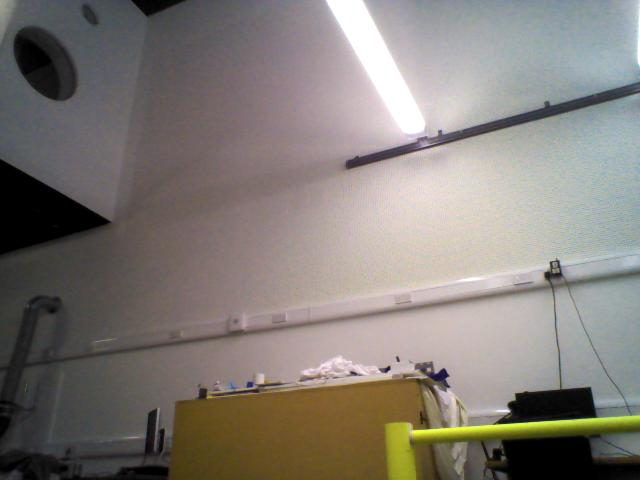
\includegraphics[scale=0.5]{../Drawings/datasetImages/mgLeft.jpg}
\caption{Dataset one showing an image from \textit{PG Left}}
\label{fig:dataset1}
\end{minipage}
\hspace{0.5cm}
\begin{minipage}[b]{0.5\linewidth}
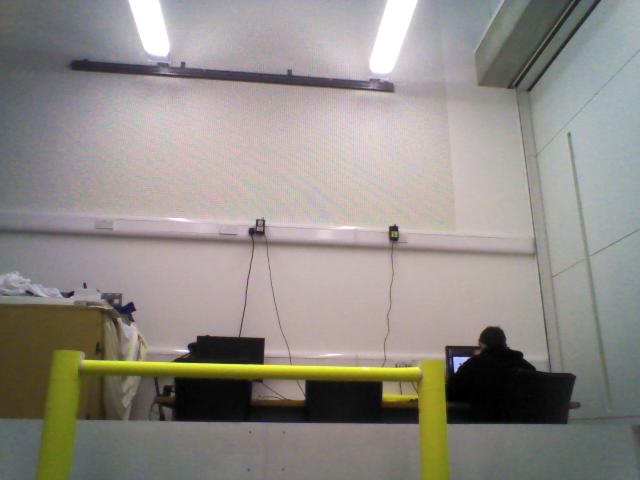
\includegraphics[scale=0.5]{../Drawings/datasetImages/mgRight.jpg}
\caption{Dataset two showing an image from \textit{PG Right}}
\label{fig:dataset2}
\end{minipage}
\hspace{0.5cm}
\begin{minipage}[b]{0.5\linewidth}
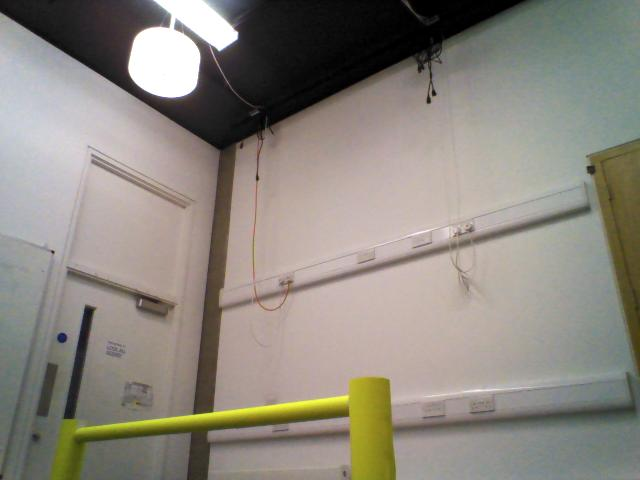
\includegraphics[scale=0.5]{../Drawings/datasetImages/ogLeft.jpg}
\caption{Dataset three showing an image from \textit{OG Left}}
\label{fig:dataset3}
\end{minipage}
\hspace{0.5cm}
\begin{minipage}[b]{0.5\linewidth}
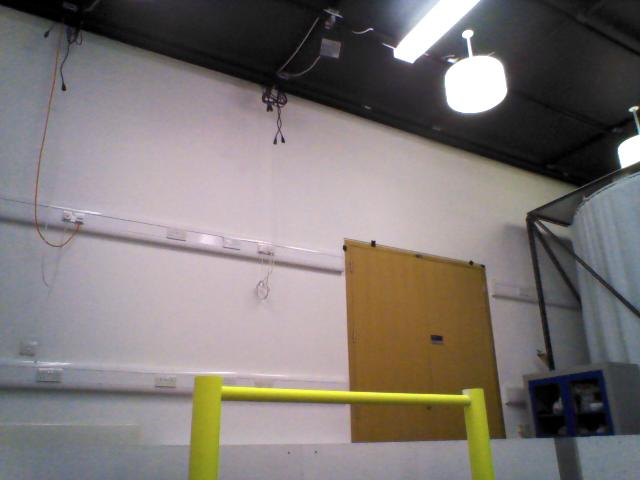
\includegraphics[scale=0.5]{../Drawings/datasetImages/ogRight.jpg}
\caption{Dataset four showing an image from \textit{OG Right}}
\label{fig:dataset4}
\end{minipage}
\end{figure}

Pairs of images taken from the same dataset are referred to as overlapping images. A pair of images are considered to overlap one another if at least $50\%$ of the first image visually overlaps the second image. This has been manually performed to ensure that the images do indeed overlap. Pairs of images with no overlap, taken from different datasets, are referred to as non-overlapping images. In order to ensure that images do not overlap, datasets from opposite sides of the soccer field were compared. Thus datasets \textit{PG Left} and \textit{PG Right} have been separately compared with datasets \textit{OG Left} and \textit{OG Right} respectively. Generating overlapping and non-overlapping image pairs has therefore been achieved by combining datasets as shown in \tabref{table:overlap}. If the same dataset appears in both columns in the table, then images within the same dataset are compared to one another generating overlapping image pairs. \\

\begin{table}
\caption{Combinations of datasets used to generate overlapping and non-overlapping image pairs in the \textit{MRE}}
\begin{tabular}{|c|c|}
\hline 
\textbf{Dataset A} & \textbf{Dataset B}\tabularnewline
\hline 
\hline 
\multicolumn{2}{|c|}{\textbf{Overlapping Images}}\tabularnewline
\hline 
MG LEFT & MG LEFT\tabularnewline
\hline 
MG RIGHT & MG RIGHT\tabularnewline
\hline 
OG LEFT & OG LEFT\tabularnewline
\hline 
OG RIGHT & OG RIGHT\tabularnewline
\hline 
\multicolumn{2}{|c|}{\textbf{Non-Overlapping Images}}\tabularnewline
\hline 
MG LEFT & OG LEFT\tabularnewline
\hline 
MG LEFT & OG RIGHT\tabularnewline
\hline 
MG RIGHT & OG LEFT\tabularnewline
\hline 
MG RIGHT & OG RIGHT\tabularnewline
\hline 
\end{tabular}
\label{table:overlap}
\end{table}

The \textit{MRE} has been used as the test environment in \secref{sec:optimalParameters} and \secref{sec:matchingProperties}. Four image datasets of regions behind the Robocup goalposts have been captured specifically for the experiments in these sections and will be referred to as the \textit{Main Robocup Parameter Datasets}. In total, these datasets collectively contain $108$ overlapping images which have been used to generate $1421$ overlapping image pairs. This is achieved by pairing all combinations of images without repetition in each image dataset. A further $108$ non-overlapping images have been used to generate $2808$ non-overlapping image pairs. The combinations of the various datasets and the number of image pairs generated are shown in \tabref{tab:mrpd}. \\

\begin{table}
\caption{Overlapping and non-overlapping image pairs generated from the \textit{Main Robocup Parameter Datasets} }
\begin{tabular}{|c|c|c|c|c|}
\hline 
\textbf{Dataset A} & \textbf{Dataset B} & \textbf{Images in A} & \textbf{Images in B} & \textbf{Image Pairs}\tabularnewline
\hline 
\hline 
\multicolumn{5}{|c}{\textbf{Overlapping Images}}\tabularnewline
\hline 
MG LEFT & MG LEFT & 26 & 26 & 325\tabularnewline
\hline 
MG RIGHT & MG RIGHT & 28 & 28 & 378\tabularnewline
\hline 
OG LEFT & OG LEFT & 31 & 31 & 465\tabularnewline
\hline 
OG RIGHT & OG RIGHT & 23 & 23 & 253\tabularnewline
\hline 
 & \textbf{Total} & 108 & 108 & 1421\tabularnewline
\hline 
\multicolumn{5}{|c}{\textbf{Non-Overlapping Images}}\tabularnewline
\hline 
MG LEFT & OG LEFT & 26 & 31 & 780\tabularnewline
\hline 
MG LEFT & OG RIGHT & 26 & 23 & 572\tabularnewline
\hline 
MG RIGHT & OG LEFT & 28 & 31 & 840\tabularnewline
\hline 
MG RIGHT & OG RIGHT & 28 & 23 & 616\tabularnewline
\hline 
 & \textbf{Total} & 108 & 108 & 2808\tabularnewline
\hline 
\end{tabular}
\label{tab:mrpd}
\end{table}

%Throughout this chapter, the term \textit{Image Match} refers to whether or not two images overlap one another. A matching of individual interest point descriptors in corresponding images will be referred to as a \textit{Match}.\\
\section{Calculating the Optimal Feature Extraction Parameters}
\label{sec:optimalParameters}
This section describes the calculation of the optimal parameters for each of the feature extraction algorithms. As mentioned previously, these parameters are calculated in the \textit{MRE} and utilise the \textit{Main Robocup Parameter Datasets}. The parameters are the MIPDT, MAHD and MAED as discussed in \secref{sec:matching}. The 1D SURF implementation does not undergo this procedure since the recommended parameter settings as defined in \cite{Anderson} have been used to perform the subsequent experiments.\\

The overlapping image pairs from the \textit{Main Robocup Parameter Datasets} are used to determine the optimal parameters for each of the feature extraction algorithms. Once the optimal parameters have been found, each feature extraction algorithm is initialised with its respective optimal parameter settings. Using these settings, the image matching performance for each algorithm is calculated on a variety of different image datasets in three different environments. The best performing algorithm can then be determined.\\


%Describes how to find the optimal hamming distance, euclidean distance, and response thresholds for each method
The procedure used to determine the optimal parameters for each of the feature extraction algorithms will now be detailed. The four image datasets, \textit{MG LEFT}, \textit{MG RIGHT}, \textit{OG LEFT} and \textit{OG RIGHT}, containing in total $108$ overlapping images, were used to determine the optimal parameter values. All possible combinations of overlapping image pairs were matched in each of the four datasets, without repetition, for various parameter values which will be mentioned below. 

For each image pair, the Single Image Score (SIS) needs to be computed. This equation is shown in \eqnref{eqn:optimalParameters}. The SIS represents how well a pair of images, $i_1, i_2$, match one another in a particular dataset $d$, for a particular Feature Extraction algorithm $FE$, using a certain set of parameters, $p$. For example, if the feature extraction algorithm used is BRISK0, then the $SIS_{(i_1, i_2), d}^{BRISK0, \textbf{p}}$ presents the SIS score for the pair of images $i_1, i_2$ for specific MIPDT and MAHD values, $p$, in a particular dataset $d$. \\

\begin{eqnarray}
SIS_{(i_1, i_2), d}^{FE, \textbf{p}} &=& \alpha f(t_{i_1,i_2}) + (1-\alpha) g(\textit{NVM}_{i_1,i_2})\\ 
\quad 0 \leq \alpha \leq 1 
\label{eqn:optimalParameters}
\end{eqnarray}

This SIS score is composed of two normalised scoring functions, namely $f(t_{i_1, i_2})$ and $g(NVM_{i_1, i_2})$ shown in \eqnref{eqn:time} and \eqnref{eqn:nvm} respectively. $f(t_{i_1, i_2})$ represents the timing score for a pair of images $i_1, i_2$ for a particular dataset based on the overall time, $t$, taken to perform the image processing, detection, extraction and matching routines respectively between these images. The unit of $t$ is milliseconds and the value of $t$ is normalised to a scale between $0$ and $1$. This is achieved by multiplying $t$ by $0.9$ and dividing this result by $t_{max}$ where $t_{max}$ is the largest time tabulated for the current dataset $d$ in milliseconds. A value of $0.1$ is then added to this ratio in order to  prevent $log(0) = \infty$ which would largely bias the results as well as ensuring that the value $(\frac{0.9 t}{t_{max}} + 0.1)$ is normalised between $0$ and $1$. The function $f(t_{i_1, i_2})$ will ensure that, for large $t$, meaning that the algorithm takes a large amount of time to perform the routine, the timing score will be low, whereas for small $t$, the timing score will be high. \\

The second scoring function used to calculate the SIS score is $g(NVM_{i_1, i_2})$. This scoring function rewards a pair of images $i_1, i_2$ if they contain a large amount of valid matches. This is intuitive as the more valid matches there are between two images, the more certain it is that the pair of images overlap one another. The variable $NVM$ represents the Number of Valid Matches (NVM) between two images. This function is normalised between $0$ and  $0.9$ by dividing this variable by the total amount of matches,$M_{total}$, generated from the pair of images $i_1, i_2$. The reason $M_{total}$ has been chosen as the normalisation factor is because it prevents a biased score. A biased score can occur in the following scenario. Assume that a pair of images $a_1, a_2$ generate a large amount of matches, but only a small proportion of these matches are valid. This is in contrast to another pair of images $b_1, b_2$ from the same dataset that generated a small set of matches, but a high proportion of valid matches. If $M_{total}$ was denoted as the maximum number of matches in the dataset, then images $b_1, b_2$ would have a smaller score than that of $a_1, a_2$ even though $b_1, b_2$ has a higher proportion of valid matches. Thus $M_{total}$ has been chosen to be the total number of matches between a pair of images $i_1, i_2$. This relative value largely prevents the biased scores. The value $\epsilon$ has been added to ensure that no infinite scores are computed. $\epsilon$ can take any value greater than $0$ and has been chosen to have a value of $0.1$, based on observation, for these experiments.\\ 

The parameter $\alpha$ is a weight that is used to bias the effects of the two scoring functions. Thus it can be used as a control to determine whether time or the number of valid matches should have a larger influence on the SIS. $\alpha$ is defined between $0$ and $1$. For these experiments, $\alpha$ was set to $0.6$. This value has been chosen as a slight bias towards faster algorithms is desired. This is because computational performance is a crucial aspect of the algorithm if it is to be implemented on the Nao robot.\\

\begin{equation}
f(t_{i_1, i_2}) = \mid log_{10}(\frac{0.9 t_{i_1, i_2}}{t_{max}^{FE}} + 0.1) \mid \quad f(t_{i_1, i_2})\in [0, 1]
\label{eqn:time}
\end{equation}

\begin{equation}
g(NVM_{i_1, i_2}) = \frac{NVM_{i_1, i_2}}{M_{total, (i_1, i_2)} + \epsilon} \quad g(NVM_{i_1, i_2}) \in [0, 1] %State that epsilon is between 0 and 1
\label{eqn:nvm}
\end{equation}

Once the SIS score has been calculated for each pair of images $i_1, i_2$, these scores are then summed together for a particular set of parameter values $p$ using a specific feature extraction algorithm $FE$ in a particular dataset $d$. The resulting score is called the Multi-Image Score (MIS) and is shown in \eqnref{eqn:mims}.\\

\begin{equation}
\tau = \frac{\sum_{i_1, i_2=1 , i_1 \neq i_2}^{N} \textit{SIS}_{(i_1, i_2),d}^{FE,p}}{N}
\label{eqn:tau}
\end{equation}

\begin{equation}
MIS_{p, d}^{FE} = \beta \tau + (1-\beta) h(\textit{IZM}) \quad 0 \leq \beta \leq 1
\label{eqn:mims}
\end{equation}

The first term of the MIS score is the computation of the mean of all SIS scores for a particular set of parameter values $p$, using a specific feature extraction algorithm $FE$, in a particular dataset $d$. This value is referred to as $\tau$ and is shown in \eqnref{eqn:tau}.\\

The second term is a scoring function that accounts for the number of Image Zero Matches (\textit{IZM}) for a particular set of parameter values. A \textit{IZM} is defined as a pair of images containing no valid matches. The function $h(IZM)$, defined in \eqnref{eqn:izm}, determines the number of \textit{IZMs} in a particular dataset $d$, for a particular set of parameter values $p$ using feature extraction algorithm $FE$. This equation has the same form as equation \eqnref{eqn:time} and therefore behaves in the same way. However, in this case the denominator $\textit{IZM}_{max}^{FE}$ represents the maximum number of IZMs found for a particular parameter setting in particular dataset using a particular feature extraction algorithm. This function therefore penalises parameter settings that result in a large number of \textit{IZM}s since \textit{IZM}s should not be present in a dataset of overlapping images. \\

\begin{equation}
h(\textit{IZM})_{p, d}^{FE} = \mid log_{10}(\frac{0.9\textit{IZM}_{p}^{FE}}{\textit{IZM}_{max}^{FE}} + 0.1) \mid \quad h(\textit{IZM}_{p}^{FE})\in [0, 1]
\label{eqn:izm}
\end{equation}

The MIS score contains a weighting parameter $\beta$ that can again be used to control the influence of each term in the function. $\beta$, like $\alpha$, is again between $0$ and $1$. $\beta$ has been set to a value of $0.4$. This creates a slight bias towards feature extraction algorithms that have a small number of IZMs. \\

\eqnref{eqn:mims} therefore provides an overall score of how well image pairs are matched for a specific setting of parameter values $p$ in dataset $d$ using feature extraction algorithm $FE$. \\

The \textit{Main Robocup Parameter Datasets} consist of four image datasets and thus  optimal parameter values are generated for each specific dataset. In order to determine the best overall set of parameters for each feature extraction algorithm, $FE$, over all datasets, two methods were utilised. The first involved finding the maximum $\textit{MIS}_{(p, d)}^{FE}$ score for each dataset, $d$, for a particular feature extraction algorithm $FE$, as well as the corresponding parameter values, $p$, that generated this \textit{MIS} score. Since there are four datasets, four sets of parameters are generated. These parameters are then averaged as shown in \eqnref{eqn:average}, and the resulting parameter values are set as the optimal parameters, $p^*$ for the feature extraction algorithm. Here, $d_i$ represents the $i^{th}$ dataset.\\

\begin{equation}
p^* = mean( max(p_{d_1}), max(p_{d_2}), max(p_{d_3}) ...) \quad d = 1,2...m
\label{eqn:average}
\end{equation}

This methodology does not necessarily produce the best set of optimal parameters. The second technique does not initially take the maximum \textit{MIS} score but first averages all corresponding \textit{MIS} scores across all datasets. A corresponding \textit{MIS} score is defined as a score that has been generated from the same parameter values but in a different dataset. Once all \textit{MIS} scores have been average across all datasets, a vector of \textit{MIS} scores results. The maximum \textit{MIS} score is then determined from this vector. This has the advantage of finding the most consistent score across all datasets rather than finding the maximum \textit{MIS} score separately for each dataset.\\

The first technique will be referred to as the \textit{Maximum Parameter Setting} (MPS). The second technique will be referred to as the \textit{Consistent Parameter Setting} (CPS).\\

Graphs showing the parameters for the CPS settings are presented in \figref{fig:BRISK0knnOptimal} to \figref{fig:BRISK0surfknnOptimal} respectively. The optimal parameter value(s) corresponding to these settings are indicated by the red lines. This has been performed for both the 2-NN and Radius Matching techniques respectively. Since the MPS settings are determined by finding the mean of four maximums as shown in \eqnref{eqn:average} from each dataset, graphs were not computed for this setting.\\

%Could possibly add in the addition of averaging the mScore matrices and then finding the maximum value. The advantage of this is to find the most consistent radius and threshold.  

%The optimal parameter graphs
\begin{figure}
\begin{minipage}[b]{0.5\linewidth}
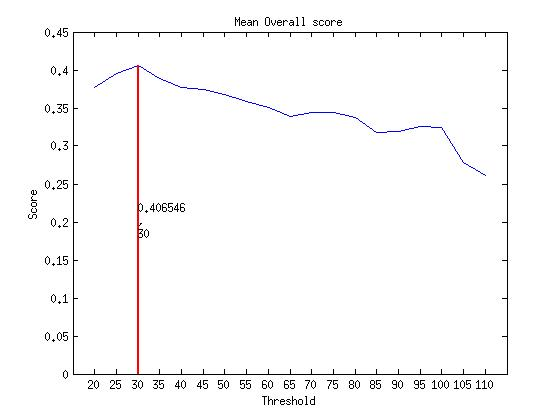
\includegraphics[scale=0.4]{../Drawings/OptimalParameters_SBRISK_SBRISK_KNN.jpg}
\caption{The optimal parameters for BRISK0 with 2-NN}
\label{fig:BRISK0knnOptimal}
\end{minipage}
\hspace{0.5cm}
\begin{minipage}[b]{0.5\linewidth}
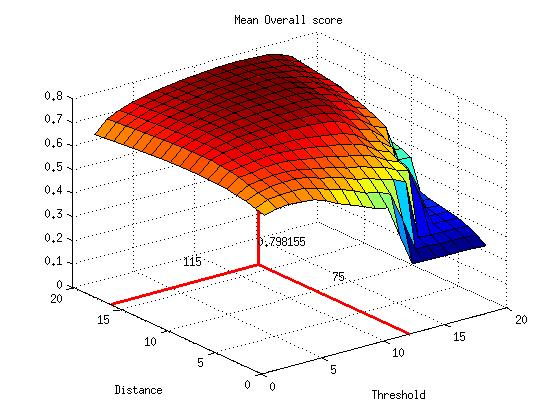
\includegraphics[scale=0.4]{../Drawings/OptimalParameters_SBRISK_SBRISK_hamming.jpg}
\caption{The optimal parameters for BRISK0 with Hamming Distance}
\label{fig:BRISK0hammingOptimal}
\end{minipage}
\begin{minipage}[b]{0.5\linewidth}
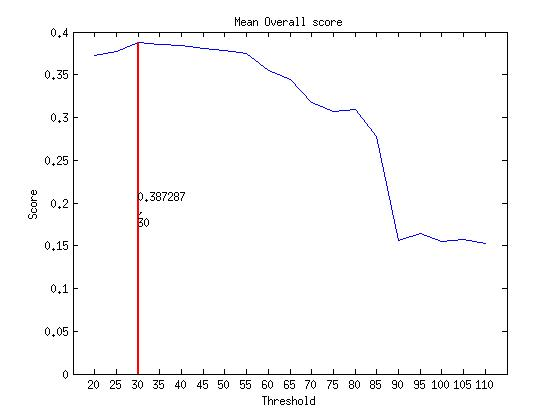
\includegraphics[scale=0.4]{../Drawings/OptimalParameters_BRISK4_BRISK4_KNN.jpg}
\caption{The optimal parameters for BRISK with 2-NN Distance}
\label{fig:BRISKknnOptimal}
\end{minipage}
\begin{minipage}[b]{0.5\linewidth}
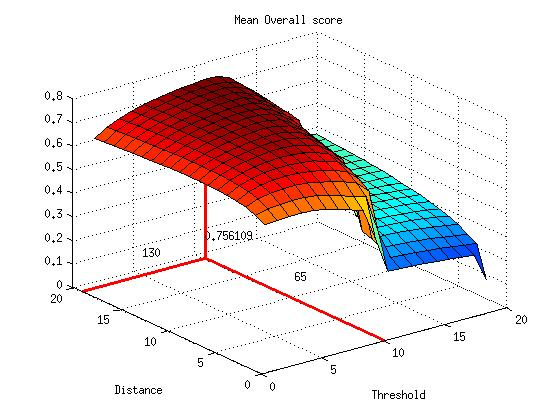
\includegraphics[scale=0.4]{../Drawings/OptimalParameters_BRISK4_BRISK4_Hamming.jpg}
\caption{The optimal parameters for BRISK with Hamming Distance}
\label{fig:BRISKhammingOptimal}
\end{minipage}
\end{figure}

\begin{figure}
\begin{minipage}[b]{0.5\linewidth}
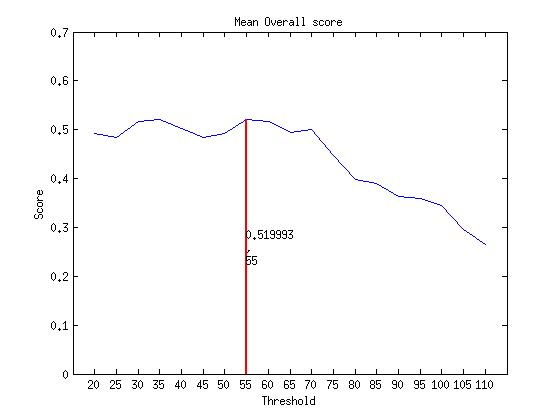
\includegraphics[scale=0.4]{../Drawings/OptimalParameters_SBRISK_SURF2D_KNN.jpg}
\caption{The optimal parameters for BRISK0 SURF2D with 2-NN}
\label{fig:BRISK0surfknnOptimal}
\end{minipage}
\hspace{0.5cm}
\begin{minipage}[b]{0.5\linewidth}
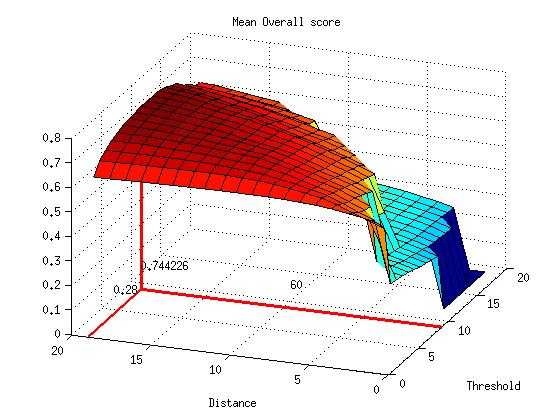
\includegraphics[scale=0.4]{../Drawings/OptimalParameters_SBRISK_SURF2D_Hamming.jpg}
\caption{The optimal parameters for BRISK0 SURF2D with Hamming Distance}
\label{fig:BRISK0surfHammingOptimal}
\end{minipage}
\begin{minipage}[b]{0.5\linewidth}
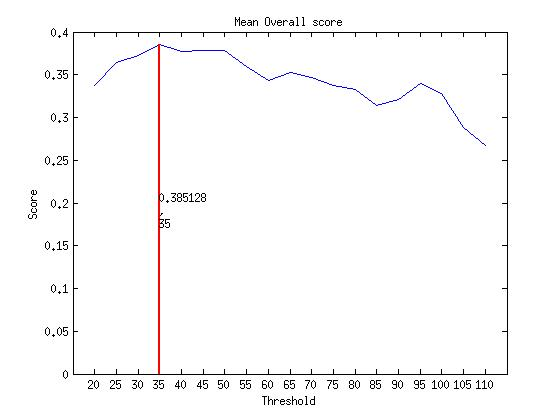
\includegraphics[scale=0.4]{../Drawings/OptimalParameters_SBRISK_UBRISK_KNN.jpg}
\caption{The optimal parameters for BRISK0 - U-BRISK with 2-NN Distance}
\label{fig:BRISK0UBRISKknnOptimal}
\end{minipage}
\begin{minipage}[b]{0.5\linewidth}
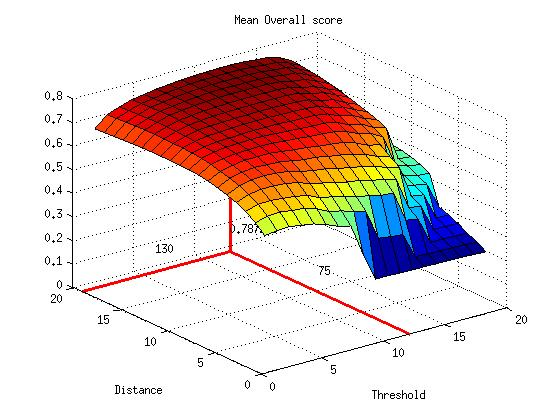
\includegraphics[scale=0.4]{../Drawings/OptimalParameters_SBRISK_UBRISK_Hamming.jpg}
\caption{The optimal parameters for BRISK0 - U-BRISK with Hamming Distance}
\label{fig:BRISK0UBRISKHammingOptimal}
\end{minipage}
\end{figure}

These experiments produced a set of optimal parameters that were generated for both the MPS and CPS parameter settings. The parameter settings are shown in \tabref{tab:knnStatistics} and \tabref{tab:hammingStatistics} for each respective matching technique. For the 2-NN tests, only the Minimum Interest Point Detection Threshold (MIPDT) parameter was varied in the range $20 \rightarrow 115$ in increments of $5$. For the Radius Matching tests, both the MIPDT and the MAHD/MAED threshold parameters were varied. The MIPDT was varied in the same range as the 2-NN tests. The MAHD is varied from $40 \rightarrow 135$ in increments of $5$ whereas the MAED is varied from $0.1 \rightarrow 0.28$ in increments of $0.01$.\\

As can be seen from the tables, the MPS parameter values tend to favour higher MIPDT thresholds compared to the CPS setting. This has the effect of detecting less interest points resulting in an increase in computational performance. In addition to this, lower MAHD/MAED values are also favoured by the MPS parameter setting which has the effect of producing less matches. In spite of these settings, a sufficient number of matches using the MPS setting are generated as will be shown in \secref{sec:overallPerformance}. This setting also increases the computational performance when computing matches between pairs of images.\\

Furthermore, both the MPS and CPS settings have been compared in three different environments as will be discussed in the sections to follow. It has been found that the MPS setting exhibits marginally better feature extraction performance in these environments. Based on this fact and since computational performance is a crucial aspect in developing a feature extraction algorithm that is suitable for real-time use on the Nao, the MPS setting will be used as the default setting for each of the relevant feature extraction algorithms. Therefore, the MPS setting is assumed to have generated the statistics unless otherwise stated in the sections to follow.\\

\begin{table}
\caption{The optimal thresholds for the 2-NN feature extraction algorithms}
\footnotesize
\begin{tabular}{|c|c|c|c|c|c|c|}
\hline 
Detector & Extractor & Matcher & $\alpha$ & $\beta$ & $MIPDT_{MPS}$ & $MIPDT_{CPS}$\tabularnewline
\hline 
\hline 
S-BRISK & S-BRISK & 2-NN & 0.6 & 0.4 & 46.25 & 30\tabularnewline
\hline 
BRISK4 & BRISK4 & 2-NN & 0.6 & 0.4 & 51.25 & 30\tabularnewline
\hline 
BRISK0 & SURF2D & 2-NN & 0.6 & 0.4 & 43.75 & 30\tabularnewline
\hline 
BRISK0 & UBRISK & 2-NN & 0.6 & 0.4 & 55 & 35\tabularnewline
\hline 
\end{tabular}
\label{tab:knnStatistics}
\end{table}

\begin{table}
\caption{The optimal thresholds for the Hamming/Euclidean distance feature extraction algorithms}
\footnotesize
\begin{tabular}{|c|c|c|c|c|c|c|c|c|}
\hline 
Detector & Extractor & Matcher & $\alpha$ & $\beta$ & $MIPDT_{MPS}$ & $MAHD_{MPS}$ & $MIPDT_{CPS}$ & $MAHD_{CPS}$\tabularnewline
 &  &  &  &  &  & $/MAED_{MPS}$ &  & $/MAED_{CPS}$\tabularnewline
\hline 
\hline 
S-BRISK & S-BRISK & Radius & 0.6 & 0.4 & 77.5 & 107.5 & 75 & 115\tabularnewline
\hline 
BRISK4 & BRISK4 & Radius & 0.6 & 0.4 & 80 & 120 & 65 & 130\tabularnewline
\hline 
BRISK0 & SURF2D & Radius & 0.6 & 0.4 & 65 & 0.28 & 60 & 0.28\tabularnewline
\hline 
BRISK0 & UBRISK & Radius & 0.6 & 0.4 & 75 & 121.25 & 75 & 130\tabularnewline
\hline 
\end{tabular}
\label{tab:hammingStatistics}
\end{table}

\section{Matching Properties}
\label{sec:matchingProperties}

\subsection{2-NN Matching Constraint}
\label{sec:knnMatchingConstraint}
In order to verify the 2-NN ratio constraint mentioned in \secref{sec:2nnMatching} and subsequently determine the optimum threshold for accepting valid matches, a number of experiments were performed using the four BRISK-based feature extraction techniques; namely BRISK0, BRISK, UBRISK and BRISK0-SURF2D. 1D SURF is not utilised since it does not use the 2-NN ratio constraint for matching.\\

In order to generate invalid matches, images with no overlap were compared, and any matches found during the comparison were flagged as invalid matches. This was performed on $2808$ non-overlapping image pairs from the \textit{Main Robocup Parameters Datasets}. To generate the valid matches, $108$ identical images from these datasets were compared and all matches found between these images were flagged as valid matches. An example of valid matches for two identical images are shown in \figref{fig:validKnn}.\\

 \begin{figure}%[ht!]
  \centering
    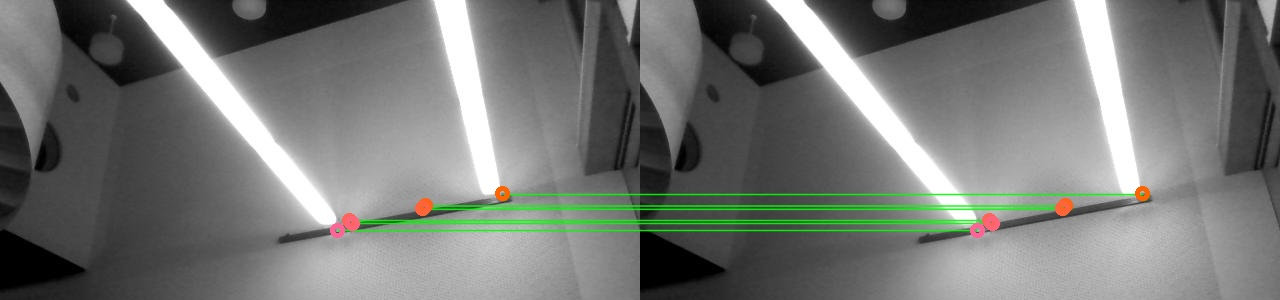
\includegraphics[width=1.0\textwidth]{../Drawings/knnRatio/KNN_ratio.jpg}
    \caption{An example of valid matches for 2-NN ratio. Only the first nearest neighbor is displayed for each interest point in this image.} 
    \label{fig:validKnn}
 \end{figure}

For both overlapping and non-overlapping images, 2-NN matching was performed generating two matches for every interest point. The distances in feature space of the first and second nearest neighbors from each interest point is then recorded. The ratio of these distances is then computed for both valid and invalid matches and the respective mean ratios are subsequently generated. The results are shown in \tabref{tab:knnCriterion} for each of the four methods. As can be seen in the table, invalid matches have a mean ratio which is over $0.9$. Valid matches have a ratio of zero for BRISK-based descriptors and $0.0004$ for the SURF2D descriptor. A ratio of zero for the BRISK-based descriptors simply means that the hamming distance between the interest point and its first nearest neighbor in a corresponding image is $0$. This is possible in identical images as shown in \figref{fig:validKnn}.\\ 

This result illustrates a significant difference between the first and second nearest neighbors for valid and invalid matches. Based on this data, all matches whose 2-NN ratio is below $0.7$ are considered valid matches whereas all matches above $0.7$ are considered to be invalid matches. This value has been chosen based on the standard deviations shown in the table in order to ensure that the majority of 2-NN invalid matches are rejected. Graphs of the 2-NN ratio for both the BRISK0 - U-BRISK method and BRISK0 method are shown in \figref{fig:b0ubknnratio} and \figref{fig:b0knnratio} respectively. \\

\begin{figure}[h!]
\begin{minipage}[b]{0.5\linewidth}
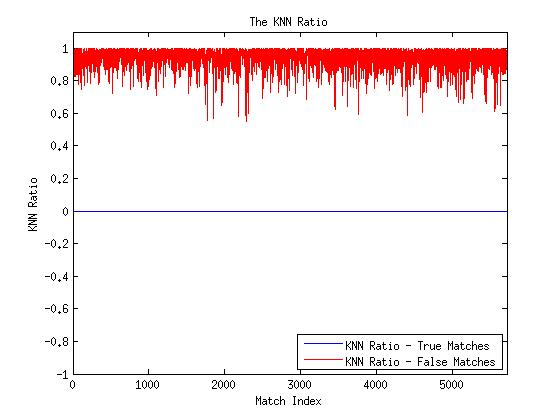
\includegraphics[scale=0.5]{../Drawings/KNNRatio_SBRISK_UBRISK_20_60.jpg}
\caption{The 2-NN ratio for non-overlapping and overlapping images respectively using the BRISK0 - UBRISK method}
\label{fig:b0ubknnratio}
\end{minipage}
\hspace{0.5cm}
\begin{minipage}[b]{0.5\linewidth}
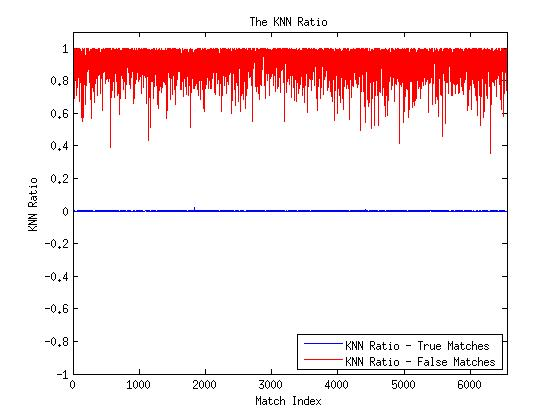
\includegraphics[scale=0.5]{../Drawings/KNNRatio_SBRISK_SURF2D_20_60.jpg}
\caption{The 2-NN ratio for non-overlapping and overlapping images respectively using the BRISK0 method}
\label{fig:b0knnratio}
\end{minipage}
\end{figure}

In addition to this, the mean distance in feature space between the first and second nearest neighbor for each algorithm has been computed. It has been found that there is a significant difference between the distances for valid and invalid matches respectively. The mean distance could also be used as a global acceptance threshold but this is not generic and some feature descriptors may be more discriminatory than others \cite{Lowe2004}. This is evident in the case of BRISK0-SURF2D whose standard deviation is $68\%$ of the total mean distance for valid matches, indicating a huge amount of fluctuation about the mean. Thus the 2-NN ratio seems to be a more robust constraint than the mean distance in this scenario.\\

\begin{table}
\caption{The 2-NN Ratios}
\footnotesize
\begin{tabular}{|c|c|c|c|c|c|}
\hline 
\textbf{Method} & \textbf{Match Type} & \textbf{Mean KNN} & \textbf{Std } & \textbf{Mean Distance } & \textbf{Std }\tabularnewline
 &  & \textbf{ Ratio} & \textbf{Deviation} & \textbf{between KNN neighbors} & \textbf{Deviation}\tabularnewline
\hline 
\hline 
\textbf{BRISK0} & Invalid Matches & 0.94 & 0.06 & 7.45 & 7.58\tabularnewline
\hline 
 & Valid Matches & 0 & 0 & 97.66 & 37.97\tabularnewline
\hline 
\textbf{BRISK} & Invalid Matches & 0.93 & 0.06 & 7.93 & 7.91\tabularnewline
\hline 
 & Valid Matches & 0 & 0 & 86.47 & 42.78\tabularnewline
\hline 
\textbf{BRISK0 - UBRISK} & Invalid Matches & 0.94 & 0.05 & 7.78 & 7.58\tabularnewline
\hline 
 & Valid Matches & 0 & 0 & 100.70 & 40.21\tabularnewline
\hline 
\textbf{BRISK0 - SURF2D} & Invalid Matches & 0.90 & 0.08 & 0.03 & 0.03\tabularnewline
\hline 
 & Valid Matches & 0.0004 & 0.0008 & 0.25 & 0.18\tabularnewline
\hline 
\end{tabular}
\label{tab:knnCriterion}
\end{table}

\subsection{Matching Score}
\label{sec:matchingScore}
As mentioned in \secref{sec:matching}, in the case of 2D SURF, interest point pairs can be matched based on the euclidean distance in feature space between interest point descriptors. Similarly, in the case of BRISK, interest points can be matched based on the hamming distance in feature space between the descriptors. In both cases, taking the inverse of this distance can produce a Matching Score (MS) as shown in \eqnref{eqn:inverseDistance}. This score has been utilised previously in \cite{AndersonTechnical, Briggs}. Here, $ip_1, ip_2$ represents the pair of interest points being compared and $D$ is the hamming/euclidean distance in feature space between the interest points' descriptors. The smaller the distance between descriptors, the more similar the interest points are, resulting in a high matching score and vice versa. In order to determine the Image Matching Score (IMS) between a pair of images, all of the individual MS values are summed together for each of the matched interest points as seen in \eqnref{eqn:ims}. Here, $i_1, i_2$ represent the image pair. \\

\begin{equation}
MS_{ip1, ip2} = \frac{1}{D_{ip1, ip2}}
\label{eqn:inverseDistance}
\end{equation}

\begin{equation}
IMS_{i1, i2} = \sum_{ip1, ip2} MS_{ip1, ip2}
\label{eqn:ims}
\end{equation}

In order to determine whether or not this score is a good metric for classifying whether images match or not, an experiment was performed. The experiment involves utilising the images from the \textit{Main Robocup Parameter Datasets} to compute the IMS for pairs of overlapping images and pairs of non-overlapping images respectively. It was expected that the IMS for the overlapping images would be larger than that of the non-overlapping images. The feature extraction algorithms utilised for this experiment include BRISK0, BRISK, BRISK0-SURF2D and BRISK0- UBRISK. Both 2-NN and Radius Matching techniques were used to calculate separate IMS values for each feature extraction algorithm.\\

The mean IMS for $1421$ overlapping images and $2808$ non-overlapping images are shown in \tabref{tab:matchingScoreCompare}. As can be seen in the table, the IMS values for overlapping images are at least an order of magnitude larger than the IMS for non-overlapping images. This indicates that \eqnref{eqn:ims} can be utilised as a means to classify whether or not a match has occurred between a pair of images. This score is one of the criteria that has been used to determine the overall performance of each of the feature extraction algorithms detailed in \secref{sec:overallPerformance}.\\

\begin{table}
\caption{The matching scores for each of the feature extraction algorithms. This is for overlapping and non-overlapping images respectively for the Main Robocup Datasets}
\begin{tabular}{|c|c|c|}
\hline 
\textbf{Method} & \textbf{Overlapping Score} & \textbf{Non-overlapping Score}\tabularnewline
\hline 
\hline 
 & 2-NN & \tabularnewline
\hline 
\textbf{BRISK0} & 0.286 & 0.003\tabularnewline
\hline 
\textbf{BRISK4} & 0.222 & 0.004\tabularnewline
\hline 
\textbf{BRISK0- SURF2D} & 77.500 & 3.259\tabularnewline
\hline 
\textbf{UBRISK} & 0.232 & 0.002\tabularnewline
\hline 
\textbf{1D SURF} & 99.756 & 31.537\tabularnewline
\hline 
 & \textbf{Radius Matching} & \tabularnewline
\hline 
\textbf{BRISK0} & 0.226 & 0.020\tabularnewline
\hline 
\textbf{BRISK4} & 0.171 & 0.006\tabularnewline
\hline 
\textbf{BRISK0- SURF2D} & 47.783 & 1.612\tabularnewline
\hline 
\textbf{UBRISK} & 0.209 & 0.010\tabularnewline
\hline 
\textbf{1D SURF} & 99.756 & 31.537\tabularnewline
\hline 
\end{tabular}
\label{tab:matchingScoreCompare}
\end{table}

It should be noted that two types of IMS scores can be generated. These are $IMS_{general}$ and $IMS_{best}$. The $IMS_{general}$ adds the MS of duplicate matches to the total IMS score. This means that if an interest point identifies two or more matches, then the MS of all of these matches will be added to the total IMS. The $IMS_{best}$ only adds the MS of the best match. Thus, even if an interest point has two or more matches, only the best match's MS will be added to the IMS value. The $IMS_{best}$ score is used as the classification threshold for determining whether or not images overlap one another. $IMS_{best}$ is also used to generate the ROC curves in the sections to follow. \\



\subsection{Properties of Valid and Invalid Matches}
\label{sec:keypointMatching}
It is also important to determine whether or not pairs of interest points generating valid matches have different properties compared to pairs of interest points generating invalid matches. This could be useful in developing new constraints that can effectively remove invalid matches. Three criteria were analysed, namely the angle $\alpha_i$, size $S_i$ and response $R_i$ of each pair of matched interest points. The subscript $i|i={1,2}$ refers to the image containing the interest point that is being evaluated. The \textit{Main Robocup Parameters Datasets} have been used for this experiment.\\

In order to generate useful statistics for this experiment, the angle, size and response of each of the interest points in image $1$ are subtracted from the angle, size and response of the corresponding matched interest points in image $2$. All of these differences are then summed together for all the matched interest points in each pair of images. The mean is subsequently computed. This results in the mean differences $\bar{d\alpha}, \bar{dS}$ and $\bar{dR}$ as shown in \eqnref{eqn:differenceProperties} respectively. The angle, response and size mean differences as well as the standard deviation for each of these differences are calculated using $40$ overlapping image pairs, $10$ from each image dataset, for the four datasets.\\

\begin{eqnarray}
\bar{d\alpha} &=& \frac{\sum_{j=1}^N (\alpha_1^j - \alpha_2^j)}{N}\\
\bar{dS} &=& \frac{\sum_{j=1}^N (S_1^j - S_2^j)}{N}\\
\bar{dR} &=& \frac{\sum_{j=1}^N (R_1^j - R_2^j)}{N}
\label{eqn:differenceProperties}
\end{eqnarray}

%The mean distance between 
In order to determine whether or not matches in images are valid, the two matching constraints discussed in \secref{sec:validation} have been utilised, namely, the angle and distance constraint and the the 2-NN ratio constraint. Utilising these constraints, overlapping image pairs were compared using the four feature extraction algorithms. \\

The interest points corresponding to valid and invalid matches generated by these constraints in each of the images were tabulated. Invalid matches due to the angle and distance constraints are tabulated separately from the invalid matches due to the 2-NN ratio constraint. The mean angle, response and size differences from the image pairs as well as the corresponding standard deviations are shown in \tabref{tab:keypointProperties}.\\

It is important to note that BRISK0 - U-BRISK and BRISK0 - 2D SURF do not output interest point angles. Thus these methods cannot be compared using the angle criterion. In addition to this, since BRISK0 only detects interest points in a single scale space, the size of the detected interest point scale remains the same. Therefore, this criterion is not used as a means of comparison for all of the BRISK0-based methods.\\

One of the more significant observations is the mean response difference $\bar{dR}$. The difference $dR$ is much smaller for valid matches compared to invalid matches over all four methods. This seems to indicate that the response of valid interest points is generally very similar.\\

In addition to this, BRISK0 and BRISK exhibit a large difference in interest point angles $\bar{d\alpha}$ for invalid matches and a much smaller difference for valid matches. \\

Finally, difference in detected scales $\bar{dS}$ has been found to be much smaller for valid matches than for invalid matches. As mentioned previously, this statistic is only valid for BRISK-based detectors with more than one octave. BRISK0 is therefore not included among these detectors.\\

Therefore, it may be possible to utilise these properties in order to further detect and remove invalid matches in images. This is a recommendation for further work on this topic.\\

%The keypoints in image A were subtracted from the keypoints in image B.

\begin{table}
\caption{The properties of valid and invalid interest point matches}
\begin{tabular}{|c|c|c|c|c|c|r@{\extracolsep{0pt}.}l|}
\hline 
\textbf{Property} & \multicolumn{7}{c}{\textbf{Invalid Matches due to Angle Constraint}}\tabularnewline
\hline 
\hline 
\textbf{Method} & \textbf{$\bar{d\alpha}$} & \textbf{$\bar{d\alpha}$Std} & \textbf{$\bar{dR}$} & \textbf{$\bar{dR}$Std} & \textbf{$\bar{dS}$} & \multicolumn{2}{c|}{\textbf{$\bar{dS}$Std}}\tabularnewline
\hline 
\textbf{BRISK0} & 20.28 & 6.68 & 0.54 & 1.07 & 0.00 & 0&00\tabularnewline
\hline 
\textbf{BRISK} & 6.98 & 1.47 & 6.31 & 2.88 & 0.30 & 2&54\tabularnewline
\hline 
\textbf{BRISK0 - SURF2D} & 0.00 & 0.00 & 0.43 & 0.89 & 0.00 & 0&00\tabularnewline
\hline 
\textbf{BRISK0 - UBRISK} & 0.00 & 0.00 & 0.13 & 2.06 & 0.00 & 0&00\tabularnewline
\hline 
 & \multicolumn{7}{c}{\textbf{Invalid Matches due to KNN Ratio Constraint}}\tabularnewline
\hline 
\textbf{BRISK0} & 4.28 & 0.87 & 6.81 & 1.98 & 0.00 & 0&00\tabularnewline
\hline 
\textbf{BRISK} & 3.24 & 4.84 & 2.43 & 1.03 & 3.02 & 4&58\tabularnewline
\hline 
\textbf{BRISK0 - SURF2D} & 0.00 & 0.00 & 2.37 & 1.70 & 0.00 & 0&00\tabularnewline
\hline 
\textbf{BRISK0 - UBRISK} & 0.00 & 0.00 & 4.61 & 1.71 & 0.00 & 0&00\tabularnewline
\hline 
 & \multicolumn{7}{c}{\textbf{Valid Matches}}\tabularnewline
\hline 
\textbf{BRISK0} & 0.66 & 0.52 & 0.08 & 0.10 & 0.00 & 0&00\tabularnewline
\hline 
\textbf{BRISK} & 1.20 & 0.31 & -0.86 & 0.05 & -0.09 & 0&41\tabularnewline
\hline 
\textbf{BRISK0 - SURF2D} & 0.00 & 0.00 & 0.29 & 0.27 & 0.00 & 0&00\tabularnewline
\hline 
\textbf{BRISK0 - UBRISK} & 0.00 & 0.00 & -0.11 & -0.44 & 0.00 & 0&00\tabularnewline
\hline 
\end{tabular}
\label{tab:keypointProperties}
\end{table}

%A picture of the graph for each method containing the optimal parameters



\section{Interest Point and Matching Statistics}
\label{sec:matchingStats}
In total, three environments have been used for comparing the various feature extraction algorithms to determine the best algorithm according to the criteria defined in \secref{sec:optimalParameters}. These include the Main Robocup Environment, the Office Environment and the Large Hall Environment. Matching statistics have been generated for each of these environments and compared for each of the feature extraction algorithms. The matching statistics have been computed for the 2-NN, Radius Matching and RANSAC matching techniques respectively. It should be noted that 1D SURF uses RANSAC and does not use 2-NN or Radius Matching. However, 1D SURF has been included as a means of comparison with the 2-NN and Radius Matching techniques. The mean number of interest points for 2-NN and Radius Matching in each of the environments is shown in \figref{fig:overall_tn_ip} and \figref{fig:overall_tn_ip_radius} respectively. The total number of matches for these techniques are presented in \figref{fig:overall_tnm} and \figref{fig:overall_tnm_radius}. Finally, the total number of valid matches are shown in \figref{fig:overall_nvm} and \figref{fig:overall_nvm_radius} respectively. These statistics will be referred to for the remainder of this section when discussing the various feature extraction algorithms and analysing their performance. As mentioned previously these statistics have been generated using the MPS values.\\

 \begin{figure}%[ht!]
  \centering
    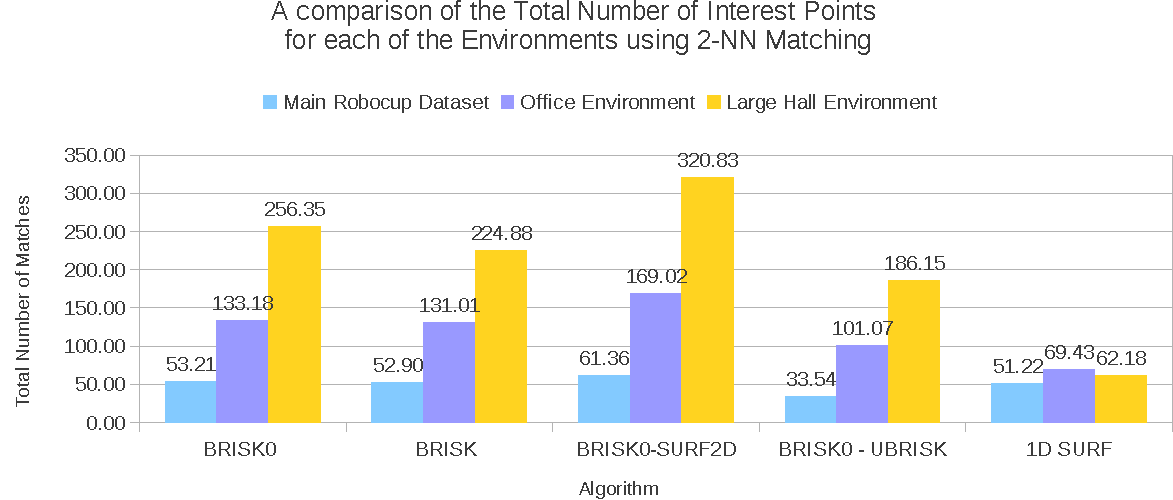
\includegraphics[width=1.0\textwidth]{../Drawings/Graphs/overall_tn_ip.pdf}
    \caption{The mean number of interest points found for each matching technique in the Main Robocup datasets} 
    \label{fig:overall_tn_ip}
 \end{figure}
 
\begin{figure}
  \centering
    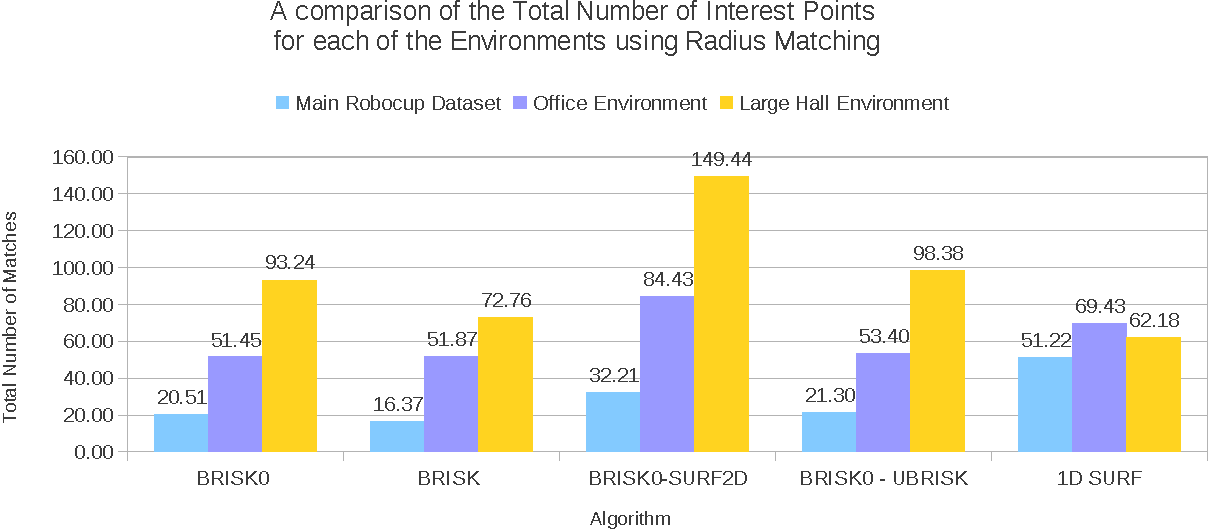
\includegraphics[width=1.0\textwidth]{../Drawings/Graphs/overall_tn_ip_radius.pdf}
    \caption{The mean number total number of matches for each matching technique in the Main Robocup datasets} 
    \label{fig:overall_tn_ip_radius}
\end{figure}

\begin{figure}
  \centering
    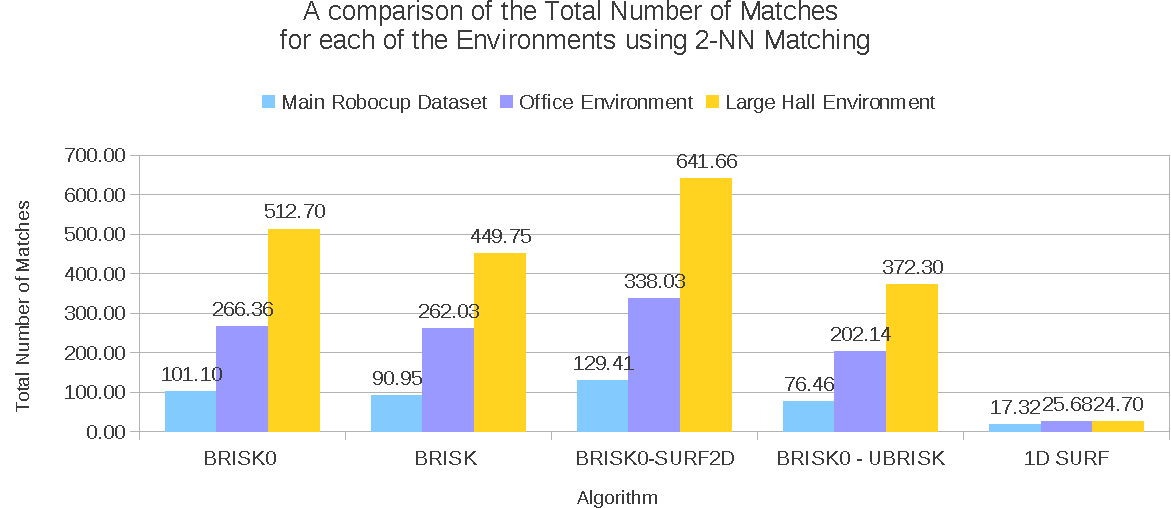
\includegraphics[width=1.0\textwidth]{../Drawings/Graphs/overall_tnm.pdf}
    \caption{The mean total number of valid matches for each matching technique in the Main Robocup datasets} 
    \label{fig:overall_tnm}
\end{figure}

\begin{figure}
  \centering
    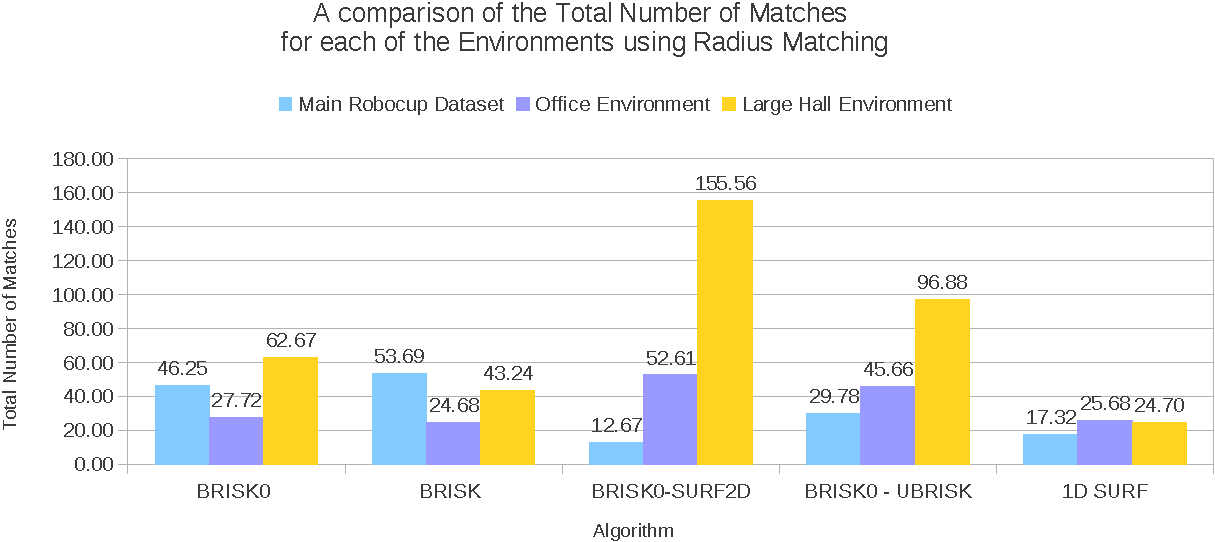
\includegraphics[width=1.0\textwidth]{../Drawings/Graphs/overall_tnm_radius.pdf}
    \caption{The mean ratio of total number of valid matches to the total number of interest points detected for each matching technique in the Main Robocup datasets} 
    \label{fig:overall_tnm_radius}
\end{figure}

\begin{figure}
  \centering
    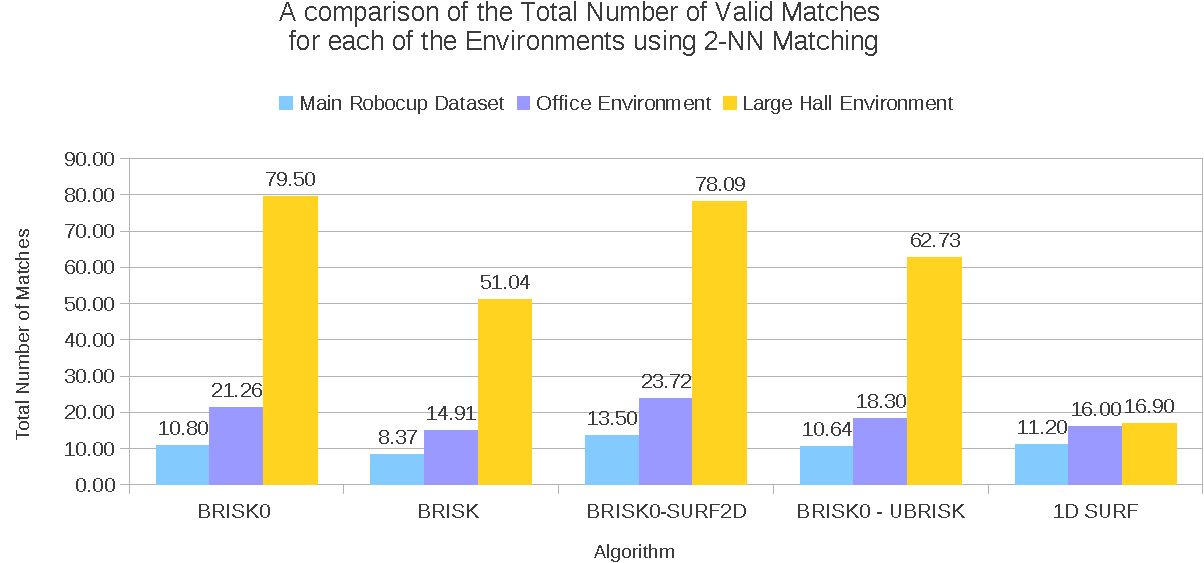
\includegraphics[width=1.0\textwidth]{../Drawings/Graphs/overall_nvm.pdf}
    \caption{The number of mean valid matches detected for non-overlapping images in the Main Robocup datasets} 
    \label{fig:overall_nvm}
\end{figure}

\begin{figure}
  \centering
    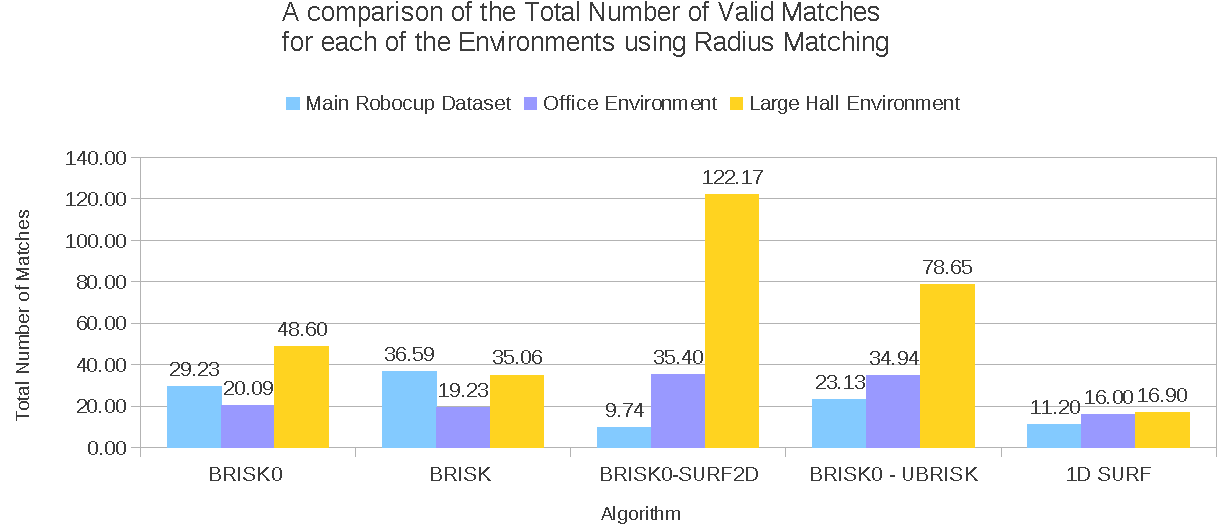
\includegraphics[width=1.0\textwidth]{../Drawings/Graphs/overall_nvm_radius.pdf}
    \caption{The number of mean valid matches detected for non-overlapping images in the Main Robocup datasets} 
    \label{fig:overall_nvm_radius}
\end{figure}

\section{Main Robocup Environment}
\label{sec:mrdPerformance}
A set of optimal parameters were previously calculated in \secref{sec:optimalParameters}. Using these parameters, each of the feature extraction algorithms have been tested in different environments in order to determine which algorithm produces the best overall performance. The first environment is the \textit{MRE}. The \textit{Main Robocup Parameter Datasets} that were used to find the optimal parameters should not be used to test the performance of the feature extraction algorithms. This would risk overfitting to the data since you would be testing the performance of the algorithms on the same data used to find the optimal parameters. Thus, a new set of datasets have been generated in the \textit{MRE}. These datasets are referred to as the \textit{Main Robocup Testing Datasets}. The datasets have the same structure as those used to calculate the optimal parameters. However, each dataset now contains $30$ images, producing in total $120$ overlapping images and $120$ non-overlapping images as shown in \tabref{tab:mrtd}. These images were then combined to create $1740$ overlapping image pairs and $3480$ non-overlapping image pairs.\\

\begin{table}
\caption{The set of overlapping and non-overlapping images generated using
the Main Robocup Validation Datasets}
\begin{tabular}{|c|c|c|c|c|}
\hline 
\textbf{Dataset A} & \textbf{Dataset B} & \textbf{Images in A} & \textbf{Images in B} & \textbf{Image Pairs}\tabularnewline
\hline 
\hline 
\multicolumn{5}{|c}{\textbf{Overlapping Images}}\tabularnewline
\hline 
MG LEFT & MG LEFT & 30 & 30 & 435\tabularnewline
\hline 
MG RIGHT & MG RIGHT & 30 & 30 & 435\tabularnewline
\hline 
OG LEFT & OG LEFT & 30 & 30 & 435\tabularnewline
\hline 
OG RIGHT & OG RIGHT & 30 & 30 & 435\tabularnewline
\hline 
 & \textbf{Total} & 120 & 120 & 1740\tabularnewline
\hline 
\multicolumn{5}{|c}{\textbf{Non-Overlapping Images}}\tabularnewline
\hline 
MG LEFT & OG LEFT & 30 & 30 & 870\tabularnewline
\hline 
MG LEFT & OG RIGHT & 30 & 30 & 870\tabularnewline
\hline 
MG RIGHT & OG LEFT & 30 & 30 & 870\tabularnewline
\hline 
MG RIGHT & OG RIGHT & 30 & 30 & 870\tabularnewline
\hline 
 & \textbf{Total} & 120 & 120 & 3480\tabularnewline
\hline 
\end{tabular}
\label{tab:mrtd}
\end{table}

Using these new datasets, the following procedure was performed. The optimal parameters (both MPS and CPS) for both the 2-NN and Radius Matching feature extraction algorithms were used as the parameter settings. Using these settings, each feature extraction algorithm was then run on all of the overlapping and non-overlapping image pairs respectively. The $IMS_{best}$, as mentioned in \secref{sec:matchingScore}, was then calculated for each image pair. It should be noted that, since the MPS values produce marginally better performance than the CPS values, the algorithms will be analysed with respect to the statistics generated using the MPS values. The CPS statistics can be found in Appendix \secref{app:cps}. \\

ROC curves have been generated for each of the five feature extraction algorithms by utilising the overlapping and non-overlapping images respectively. The threshold used for classifying whether or not two images match one another is the $IMS_{best}$. This implies that interest points with duplicate matches will only contribute their best match (lowest hamming/euclidean distance in feature space) to the $IMS_{best}$. \\

Overlapping images generate the True Positive (TP) matches. The $IMS_{best}$ threshold is varied in a range from the maximum $IMS_{best}$ in the datasets to $0$.  All overlapping image pairs with a larger $IMS_{best}$ than the $IMS_{best}$ threshold are classified as matching one another and all overlapping image pairs below the $IMS_{best}$ threshold are classified as not matching one another. The False Positives (FP) are generated from the non-overlapping image pairs. Again, the $IMS_{best}$ threshold is varied along the same range and all non-overlapping image pairs above the threshold are defined as matching one another and vice versa. If a non-overlapping image pair is defined as a match, then it is a FP. The ROC curves for the five algorithms are shown in \figref{fig:compareHamming} and \figref{fig:compareKNN}.\\

\figref{fig:compareHamming} shows the ROC curves for the five methods using Radius Matching, and MPS values which were calculated in \secref{sec:optimalParameters}. \figref{fig:compareKNN} shows the ROC curves for 2-NN Matching, using the MPS values. Area Under the ROC Curve (AUC) values have been calculated for each of the ROC curves and are presented in \tabref{tab:mrd_times_knn} and \tabref{tab:mrd_times_hamming} respectively. This table also contains the average performance times corresponding to each section of the feature extraction algorithms. The detection time is defined as the amount of time required to detect all of the interest points in a single detector module. The extraction time is the time taken to compute the descriptors of the detected interest points for a single descriptor module. The matching time is the time taken to match all of the interest points for a single pair of images. The verification time is the time taken to detect and remove invalid interest points. Finally the overall time is the summation of these times as well as the time taken to process and extract the image from the robot. These statistics will now be analysed for each feature extraction algorithm. \\

\begin{figure}[h!]
\begin{minipage}[b]{0.5\linewidth}
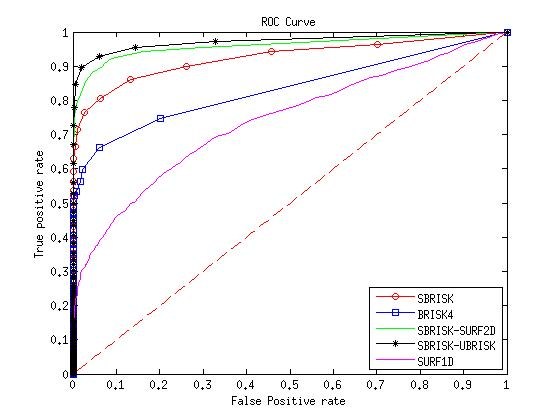
\includegraphics[scale=0.4]{../Drawings/RobocupDataset/ROC_General_Hamming_max.jpg}
\caption{A comparison of the ROC curves for the Robocup datasets using Radius Matching and MPS values}
\label{fig:compareHamming}
\end{minipage}
\hspace{0.5cm}
\begin{minipage}[b]{0.5\linewidth}
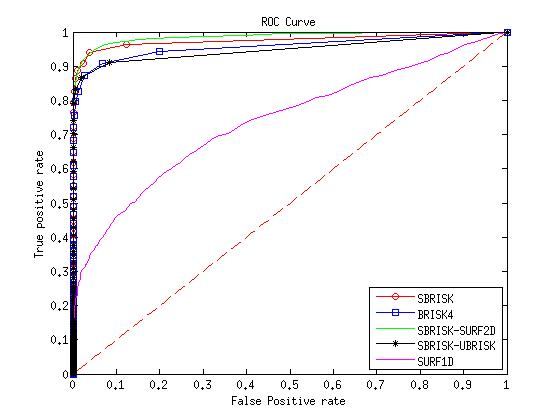
\includegraphics[scale=0.4]{../Drawings/RobocupDataset/ROC_General_KNN_max.jpg}
\caption{A comparison of the ROC curves for the Robocup datasets using 2-NN for matching and MPS values}
\label{fig:compareKNN}
\end{minipage}
\end{figure}



\begin{table}
\caption{The AUC and performance statistics for the Main Robocup Dataset using
2-NN}
\footnotesize
\begin{tabular}{|c|c|c|c|c|c|c|c|}
\hline 
\textbf{Method (2-NN)} & \textbf{Parameters} & \textbf{\% AUC} & \textbf{Detection} & \textbf{Extraction} & \textbf{Matching} & \textbf{Verification} & \textbf{Overall}\tabularnewline
 &  &  & \textbf{Time (ms)} & \textbf{Time (ms)} & \textbf{Time (ms)} & \textbf{Time (ms)} & \textbf{Time (ms)}\tabularnewline
\hline 
\hline 
BRISK0 & MPS & 97.407 & 3.348 & 4.766 & 0.942 & 0.022 & 13.073\tabularnewline
\hline 
BRISK4 & MPS & 95.039 & 10.007 & 4.555 & 0.807 & 0.021 & 19.415\tabularnewline
\hline 
BRISK0-SURF2D & MPS & 98.654 & 3.432 & 9.312 & 0.359 & 0.028 & 17.179\tabularnewline
\hline 
\textbf{BRISK0-UBRISK} & \textbf{MPS} & \textbf{95.356} & \textbf{3.224} & \textbf{2.244} & \textbf{0.588} & \textbf{0.018} & \textbf{10.049}\tabularnewline
\hline 
\textbf{SURF 1D} & \textbf{Given} & \textbf{74.039} & \textbf{0.271} & \textbf{0.134} & \textbf{0.242} & \textbf{0.030} & \textbf{13.301}\tabularnewline
\hline 
\end{tabular}
\label{tab:mrd_times_knn}
\end{table}

\begin{table}
\caption{The AUC and performance statistics for the Main Robocup Dataset using
Radius Matching}
\footnotesize
\begin{tabular}{|c|c|c|c|c|c|c|c|}
\hline 
\textbf{Method (2-NN)} & \textbf{Parameters} & \textbf{\% AUC} & \textbf{Detection} & \textbf{Extraction} & \textbf{Matching} & \textbf{Verification} & \textbf{Overall}\tabularnewline
 &  &  & \textbf{Time (ms)} & \textbf{Time (ms)} & \textbf{Time (ms)} & \textbf{Time (ms)} & \textbf{Time (ms)}\tabularnewline
\hline 
\hline 
BRISK0 & MPS & 92.455 & 2.965 & 2.608 & 0.207 & 0.012 & 9.734\tabularnewline
\hline 
BRISK4 & MPS & 83.290 & 7.870 & 2.556 & 0.161 & 0.010 & 14.627\tabularnewline
\hline 
BRISK0-SURF2D & MPS & 96.033 & 3.115 & 5.711 & 0.192 & 0.007 & 13.027\tabularnewline
\hline 
\textbf{BRISK0-UBRISK} & \textbf{MPS} & \textbf{97.242} & \textbf{2.973} & \textbf{1.672} & \textbf{0.207} & \textbf{0.008} & \textbf{8.805}\tabularnewline
\hline 
\textbf{SURF 1D} & \textbf{Given} & \textbf{74.039} & \textbf{0.271} & \textbf{0.134} & \textbf{0.242} & \textbf{0.030} & \textbf{13.301}\tabularnewline
\hline 
\end{tabular}
\label{tab:mrd_times_hamming}
\end{table}

BRISK0 is able to achieve comparatively fast times achieving a best time of $9.73 ms$ when using Radius Matching and the MPS values. This is not as fast as BRISK0 - U-BRISK since the BRISK0 algorithm is rotation invariant and therefore has to rotate the sampling pattern around the interest point as defined in \secref{sec:brisk}. This causes a larger extraction time as can be seen in \tabref{tab:mrd_times_knn} and \tabref{tab:mrd_times_hamming}.\\

The BRISK0 algorithm detects on average $53.21$ and $20.51$ interest points for both 2-NN and Radius Matching respectively as seen in \figref{fig:overall_tn_ip} and \figref{fig:overall_tn_ip_radius}. It must be noted that a different number of interest points have been detected for 2-NN Matching and Radius Matching since these techniques operate using different MPS values. \\

This algorithm achieves good performance when utilising 2-NN matching, attaining an AUC value of $97.41\%$ using MPS values as seen in \tabref{tab:mrd_times_knn}. One of the reasons for large AUC values are the number Image of Zero Matches (IZMs) that are generated by a feature extraction algorithm. As mentioned previously, an IZM means that a pair of images contain zero valid interest point matches. If an overlapping pair of images contain zero valid matches, then the $IMS_{best}$ score will be $0$ for this image pair. Thus when computing the ROC curve, only once the $IMS_{best}$ threshold reaches zero, will this pair of images be classified as an image match. This ultimately reduces the AUC value as the TP rate is reduced, and IZMs are therefore undesirable for overlapping images. On the other hand, it is desirable for every non-overlapping image pair to have zero valid matches as these images do not overlap and therefore should not match. Thus datasets of non-overlapping images should ideally have a large value of IZMs.\\

BRISK0 generates $60$ and $55$ IZMs for MPS values using 2-NN and Radius Matching respectively as seen in \tabref{tab:mrd_izm}. This is a comparatively low number of IZMs and therefore is one of the reasons why large AUC values result as tabulated in \tabref{tab:mrd_times_knn} and \tabref{tab:mrd_times_hamming}. One of the possible reasons why BRISK0 has a low number of IZMs is due to the fact that it only performs non-maximal suppression in an image neighborhood on a single octave. This causes weak interest points to be detected. Weak interest points are those that are significantly brighter or darker than their surrounding neighborhood of pixels on a single octave only. As a result of relaxing the non-maximal suppression constraint, more interest points will be detected, decreasing the chances of an image pair becoming an IZM. This can cause a problem whereby weak interest points are incorrectly matched and this will be elaborated on in \secref{sec:discussionConclusion}. An example of weak interest points that are correctly matched is shown in \figref{fig:weakMatch}.\\

 
\begin{figure}
  \centering
    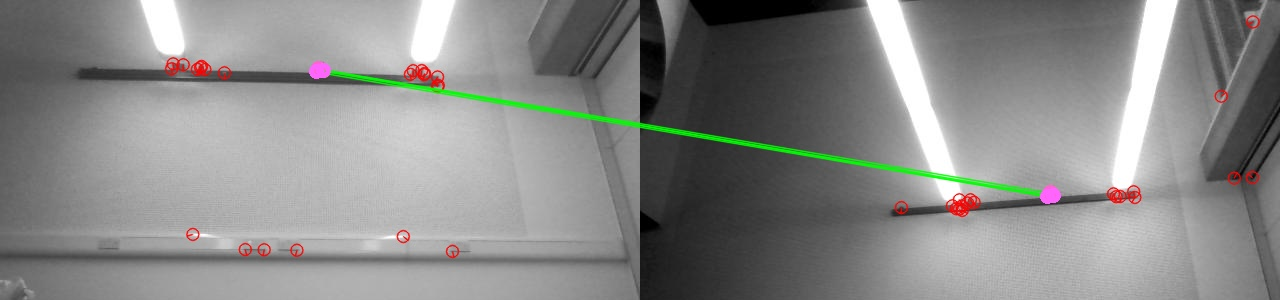
\includegraphics[width=1.0\textwidth]{../Drawings/Matching/weakInterestPointMatch.jpg}
    \caption{Weak interest points matched using the BRISK0 implementation} 
    \label{fig:weakMatch}
\end{figure}

In addition to this, the $IMS_{best}$ for overlapping and non-overlapping images needs to be analysed. As can be seen in \tabref{tab:matchingScoreCompare}, the mean IMS for BRISK0 is at least an order of magnitude larger for overlapping images compared to non-overlapping images. A graph has been generated in \figref{fig:ms_brisk0}, plotting the $IMS_{best}$ of overlapping images and non-overlapping images' $IMS_{best}$ respectively. As can be seen in the figure, as the $IMS_{best}$ threshold is varied from the maximum value to zero, the TP rate will consistently increase as overlapping images will be classified as image matches. Only near very low thresholds will the FP rate begin to increase as non-overlapping images will begin to be classified as image matches. This contributes to the large AUC value. It will be shown in \secref{sec:zfp} that even though the overlapping $IMS_{best}$ values have a large amount of variation as seen in the figure, a suitable separation boundary can be established that enables BRISK0 to match pairs of overlapping images and reject pairs of non-overlapping images to a reasonable degree of accuracy.\\

\begin{figure}
  \centering
    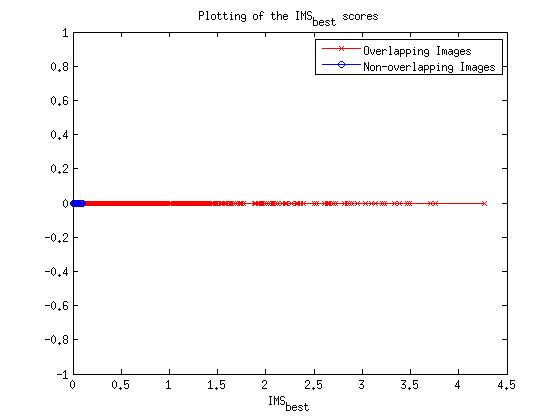
\includegraphics[width=0.8\textwidth]{../Drawings/Matching/MatchingScore_BRISK0.jpg}
    \caption{The $IMS_{best}$ values of overlapping and non-overlapping image pairs in red and blue respectively.} 
    \label{fig:ms_brisk0}
\end{figure}

BRISK0's Radius Matching performance is slightly worse in comparison as seen in \tabref{tab:mrd_times_hamming} achieving an AUC of $92.45\%$. This is due an increase in the $IMS_{best}$ value, from $0.003$ to $0.02$, for non-overlapping images as seen in \tabref{tab:matchingScoreCompare}. This implies that more interest points are matched in non-overlapping images. This is possible since the 2-NN ratio constraint is not applied for Radius Matching which may result in invalid interest points being matched in non-overlapping images.\\

This scenario can occur if a pair of non-overlapping images have similar features such as lights, plug sockets or dangling wires. Interest points in these regions can generate a large number of incorrect matches causing a larger $IMS_{best}$ value for the non-overlapping image pair. An example of this is shown in \figref{fig:duplicateMatchesBrisk0} where the lights have caused multiple incorrect matches between non-overlapping images. An interest point located at one of the ceiling lights will tend to match with interest points located on any of the other lights in the corresponding image. This is because the intensities are very similar in the neighborhoods surrounding these interest points resulting in duplicate matches. As a result of the larger mean non-overlapping $IMS_{best}$ value, the AUC will decrease as seen in \figref{fig:compareHamming}.\\

\begin{figure}
  \centering
    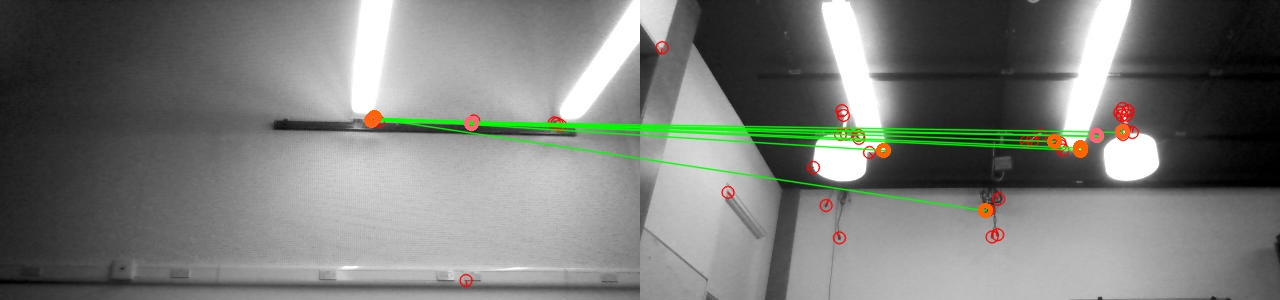
\includegraphics[width=1.0\textwidth]{../Drawings/Matching/fpMatchBRISK0.jpg}
    \caption{FP matches due to the lighting in the image for the BRISK0 algorithm} 
    \label{fig:duplicateMatchesBrisk0}
\end{figure}

One final point to note about the BRISK0 algorithm is that it contains an unusually large number of total matches when using Radius Matching as seen in \figref{fig:overall_tnm_radius}. This number is unusual since the \textit{Office Environment} and \textit{Large Hall Environment} have more salient features and therefore detect more interest points as shown in \figref{fig:overall_tn_ip_radius}. The reason for the large number of matches when using Radius Matching is due to reflections as well as lights as shown in \figref{fig:reflectionsBrisk0}. Since the lights and reflections of the fluorescent lights create similar intensity neighborhoods, a large number of duplicate matches result. Radius Matching does not limit the number of matches causing a large number of interest points to be detected.\\

\begin{figure}
  \centering
    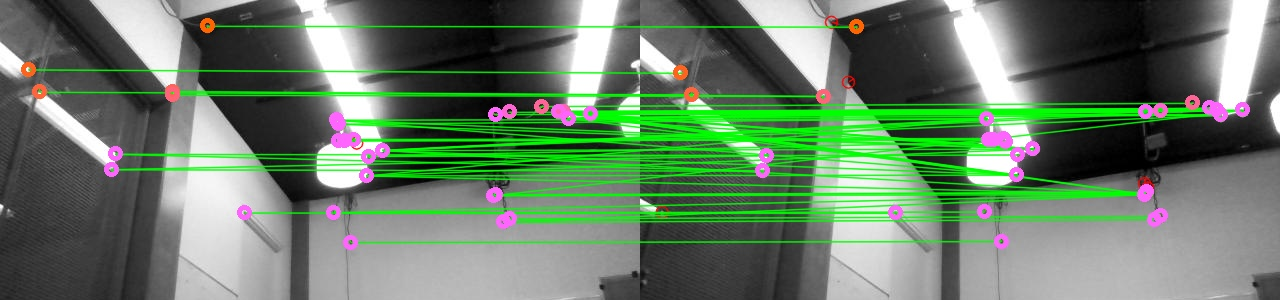
\includegraphics[width=1.0\textwidth]{../Drawings/Matching/reflectionsBrisk0.jpg}
    \caption{FP matches due to lighting and reflections in overlapping images} 
    \label{fig:reflectionsBrisk0}
\end{figure}


The BRISK algorithm has a large feature detection time as seen in \tabref{tab:mrd_times_knn} and \tabref{tab:mrd_times_hamming}. This is because the method is calculating features across multiple scales. A 3D interpolation is also performed as mentioned previously in order to generate continuous scale refinements. This is a time consuming operation and results in the large detection times seen in the tables. As a result, BRISK is the slowest of the five algorithms and achieves a best overall time of $14.62 ms$ when using Radius Matching and the MPS values.\\

BRISK detects on average $45.47$ interest points when using 2-NN matching and $16.37$ interest points when using Radius Matching. The small amount of interest points detected when performing Radius Matching is partially due to the MPS values. The MIPDT threshold is higher than the other algorithms enabling BRISK to only detect strong interest points and therefore salient features. In addition to this, the non-maximal suppression across multiple scales reduces the amount of interest points that can be detected.\\

In the 2-NN Matching experiments, the matching performance of the algorithm achieves a comparatively large AUC value of $95.04\%$. This is less than BRISK0 and can be explained by the number of IZMs for overlapping image pairs generated from this algorithm. As can be seen in \tabref{tab:mrd_izm}, BRISK has $105$ IZMs for overlapping image pairs and therefore results in a smaller AUC value. After analysing the data, it was found that the increase in IZMs is due to the non-maximal suppression constraint and the large MIPDT value. This reduces the number of detected interest points and causes overlapping image pairs to have very few and often $0$ interest points and therefore produces no matches. An example of this scenario is seen in \figref{fig:noMatchesBrisk4}. The left image in the figure has very few interest points and does not match any of these points with the right image even though the two images overlap.\\

\begin{figure}
  \centering
    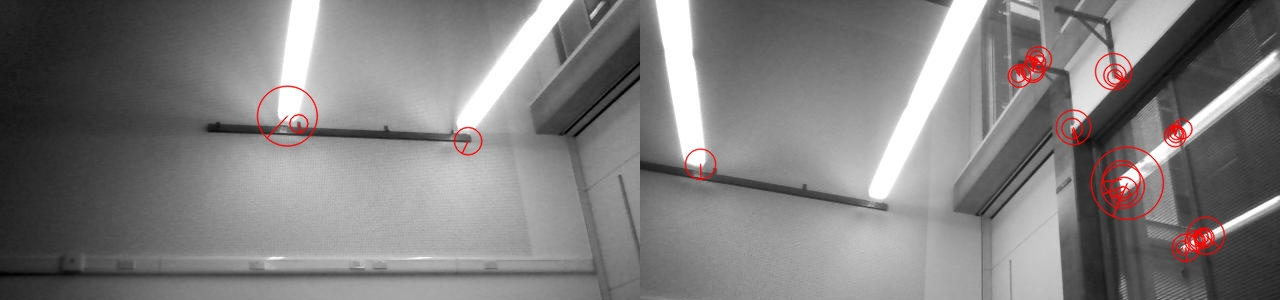
\includegraphics[width=1.0\textwidth]{../Drawings/Matching/noMatchesBrisk4.jpg}
    \caption{No matches in overlapping images resulting from very few interest points being detected for the BRISK4 algortihm }
    \label{fig:noMatchesBrisk4}
\end{figure}

The BRISK technique does not produce a large AUC when utilising Radius Matching. It achieves a  value in this case of $83.29\%$ which is one of the lower AUC values compared to the other feature extraction algorithms. This may seem to be a strange outcome since this algorithm detects the largest number of matches as shown in \figref{fig:overall_tnm_radius}. However, the core of the problem arises from the number of IZMs that are generated for overlapping image pairs. As can be seen in \tabref{tab:mrd_izm}, BRISK has $402$ IZMs. In addition to this, the MIPDT value has been increased to $80$ for the MPS values as seen in \tabref{tab:hammingStatistics}. This causes fewer interest points to be detected resulting in less valid matches and poor performance. The reason for the increase in the MIPDT value is due to the optimal parameters algorithm discussed in \secref{sec:optimalParameters} requiring efficient computational performance at an expense in matching performance. Since BRISK is the slowest of the algorithms, it can only achieve good computational performance by having higher thresholds and therefore less interest points being detected.\\

Reflections and lights again cause a problem for BRISK resulting in a large number of duplicate matches respectively as shown in \figref{fig:overall_tnm_radius}. The duplicate matches are generally detected on or near the ceiling lights as shown in \figref{fig:duplicateMatchesBrisk}. Areas near the lights will have similar intensities and this causes the incorrect detection of interest points.\\

\begin{figure}
  \centering
    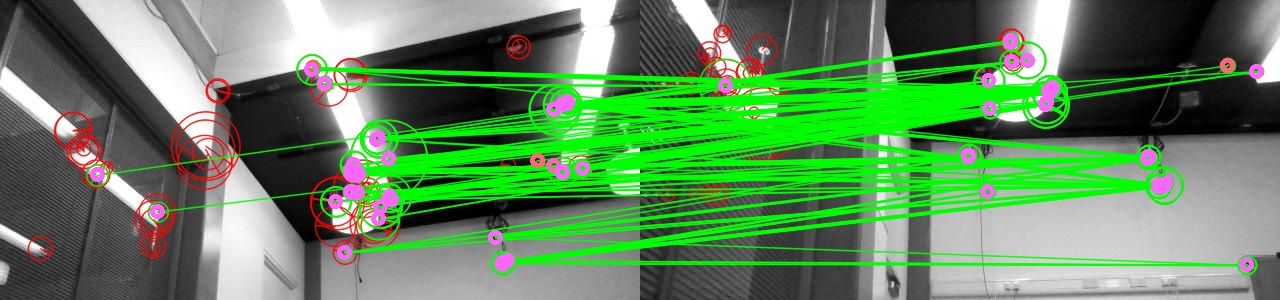
\includegraphics[width=1.0\textwidth]{../Drawings/problems/Reflections.jpg}
    \caption{Duplicate matches due to the lighting in the image as well as reflections for the BRISK0 algorithm} 
    \label{fig:duplicateMatchesBrisk}
\end{figure}



In terms of speed, BRISK0 - U-BRISK is the best performing algorithm with a best overall time of $8.81 ms$ as seen in \tabref{tab:mrd_times_hamming} using the Radius Matching technique.  This is expected since a number of constraints have been relaxed. These include the single scale constraint as well as removing rotation invariance as mentioned in \secref{sec:brisk0}. These constraints have been relaxed in order to maximise computational efficiency and therefore satisfy the computational requirements of the Nao robot. This method therefore has the fastest extraction time of $1.67 ms$ as the sampling pattern is not rotated in this variation of the BRISK technique. \\

The BRISK0 - U-BRISK algorithm detects on average $38.23$ and $21.30$ interest points for 2-NN and Radius Matching respectively as shown in \figref{fig:overall_tn_ip} and \figref{fig:overall_tn_ip_radius}. When using 2-NN matching, this algorithm achieves an AUC value of $95.35\%$. This is relatively low compared to the other feature extraction algorithms for 2-NN matching. This is due to the algorithm having the largest number of IZMs. It has $108$ IZMs as shown in \tabref{tab:mrd_izm}. This is expected, since this method is not rotation invariant since the sampling pattern is not rotated in order to achieve better computational performance. This causes a number of matches to be lost since large image rotations cause corresponding interest points to be set at different orientations which may prevent these points from being matched. To prove this, an identical image was considerably rotated and compared with its unrotated version as shown in \figref{fig:rotationUbrisk}. An interest point has been identified between both of the fluorescent lights in each image but the interest point has not been matched due to this rotation. However, since the Nao will not be subject to large rotations when coming onto the pitch after serving a penalty ban in the Robocup environment, this method is still a feasible option. \\

\begin{figure}
  \centering
    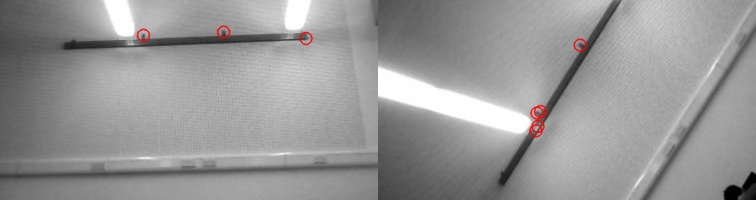
\includegraphics[width=1.0\textwidth]{../Drawings/Matching/rotationsUBRISK.jpg}
    \caption{Matches lost due to BRISK0 - U-BRISK being rotation variant} 
    \label{fig:rotationUbrisk}
\end{figure}

%When using 2-NN matching, this method achieves an AUC value of $87.83\%$ as seen in \tabref{tab:overall_times_knn}. This algorithm also has a small number of FP matches as seen in \figref{fig:mrd_nvm_nol}. This results in a lower matching score for non-overlapping images which ultimately produces a larger AUC value since there is a large difference between the overlapping matching score and the non-overlapping matching score as shown in \tabref{tab:matchingScoreCompare}. 

This algorithm produces very good classification performance when using Radius Matching as an AUC value of $97.24\%$ is achieved. This good performance is mainly due the lower number of IZMs. This value has significantly decreased for Radius Matching to a mean value of $33$ for overlapping image pairs. This is mainly due to the MPS's MAHD value that determines the threshold, below which, two interest point descriptors match one another. This value causes an increase in the number of detected matches resulting in the improved performance.\\

The $IMS_{best}$ is again at least an order of magnitude higher for overlapping images than for non-overlapping images which generates a larger TP rate. A graph showing the separation of matching scores is shown in \figref{fig:ms_ubrisk}. Again, it can be seen that non-overlapping image pairs have a very low $IMS_{best}$ compared to overlapping images. Even though the IMS for overlapping images have a large amount of variation, it will be shown in \secref{sec:zfp} that a suitable separation boundary can be established that enables BRISK - U-BRISK to effectively match pairs of overlapping images and reject pairs of non-overlapping images.\\

\begin{figure}
  \centering
    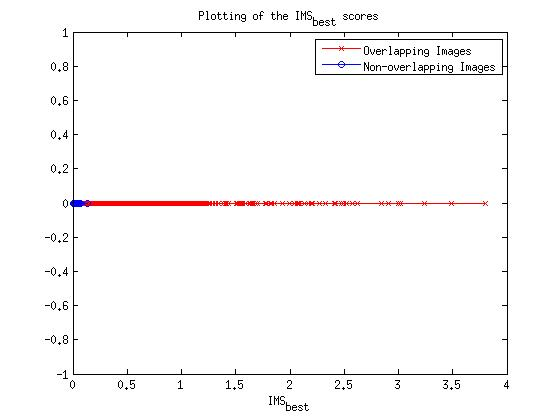
\includegraphics[width=0.8\textwidth]{../Drawings/Matching/MatchingScore_BRISK0UBRISK.jpg}
    \caption{The $IMS_{best}$ for overlapping images in red and non-overlapping images in blue.} 
    \label{fig:ms_ubrisk}
\end{figure}

BRISK0 - SURF2D has better computational performance than BRISK but still suffers as this method has a large extraction time. This is because 2D SURF descriptors are computed which are computationally expensive. This includes calculating Haar Wavelet Responses in both the $x$ and $y$ directions in each of the sub-regions defined around the interest point. These responses then have to be summed as described in \secref{sec:2dsurf} to form the interest point descriptor. However, since BRISK0 is being utilised in detecting interest points, this algorithm is marginally faster than BRISK.\\

BRISK0 - 2D SURF detects on average $64.71$ and $32.21$ interest points for 2-NN matching and Radius matching respectively as seen in \figref{fig:overall_tn_ip} and \figref{fig:overall_tn_ip_radius}. These are the most interest points detected compared to the other BRISK-based algorithms and can be explained by noting that this algorithm uses the lowest MIPDT threshold of $43.75$ when detecting interest points. \\

As can be seen in \tabref{tab:mrd_times_knn} and \tabref{tab:mrd_times_hamming}, the algorithm producing the marginally best AUC is BRISK0 - 2D SURF with a value of $98.64\%$. This performance is achieved when utilising 2-NN matching. This is partly due to the fact that this algorithm produces only $7$ IZMs which is the lowest of all the algorithms. This is due to the low MIPDT threshold which enables more interest points to be detected as can be seen in \figref{fig:overall_tn_ip}. This results in more matches as shown in \figref{fig:overall_tnm} and this produces the largest mean number of valid matches as seen in \figref{fig:overall_nvm}.\\

In addition to this the $IMS_{best}$ value for overlapping image pairs is at least an order of magnitude larger than the $IMS_{best}$ value for non-overlapping image pairs which yields the above-mentioned classification performance. \\

The AUC value decreases slightly to $96.03\%$ when utilising Radius Matching. One reason for this drop is the increase in the number of IZMs to a value of $77$. This seems to be due to the MAED threshold chosen for this algorithm of $0.28$ as seen in \tabref{tab:hammingStatistics}. The range for this threshold may need to be increased in the optimisation algorithm detailed in \secref{sec:optimalParameters} in order to allow for more interest points to be detected. However, fairly good performance is still maintained since there is a large gap, by more than an order of magnitude, between the overlapping matching scores and the non-overlapping matching scores respectively. \\

%This is partially due to the fact that the BRISK4 algorithm detects interest points by performing a non-maximal suppression over scale space. This filters out more interest points as these points have to fulfil a more demanding constraint than that imposed in the BRISK0 implementation. The BRISK0 implementation simply detects interest points if they are not suppressed in a single scale dimensional.\\


In terms of overall speed, the 1D SURF algorithm has the fastest extraction and detection times by an order of magnitude compared to the BRISK-based techniques as seen in \tabref{tab:mrd_times_knn} and \tabref{tab:mrd_times_hamming}. This is because interest points are only detected along a single dimension which creates a very fast detection time. The extraction time is also very efficient since Haar Wavelet Responses are only calculated in the $x$ direction and a feature descriptor of length $6$ is generated as opposed to the $64$ length descriptor generated by 2D SURF. It should be noted that the mean overall time taken to determine whether an image pair matches or not is slower than BRISK0 - U-BRISK. However, this can definitely be increased in order to perform more efficiently than the BRISK-based techniques.\\

This algorithm detects on average $51.22$ interest points. However,the 1D SURF technique seems to struggle in this environment as it only manages to attain an AUC of $74.04\%$. It is possible that since there is a small amount of variation in the scene, there may be a problem identifying unique features since the single row of pixels may have a large number of similar pixel values. Evidence to support this claim can be seen in \figref{fig:ambiguities} where pixels are matched with the fluorescent light on the left hand side of the upper left image. Since this algorithm seems to have been designed for areas containing a significant amount of variation as presented in \cite{Anderson}, some further additions may be necessary in order to adjust the algorithm such that it can efficiently detect features in images containing low variation. There is an improvement in performance when matching pairs of images in the \textit{Office Environment} and \textit{Large Hall Environment} due to the significant amount of variation in the images as will be discussed in \secref{sec:additionalDataset}.\\

\begin{figure}
  \centering
    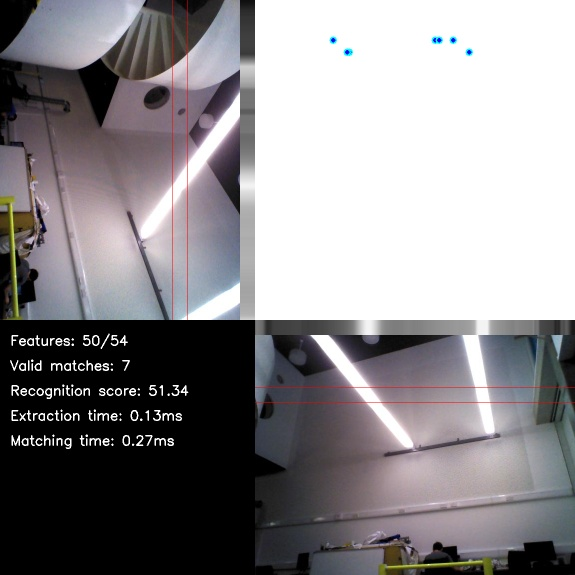
\includegraphics[width=0.8\textwidth]{../Drawings/Matching/nonmatching.jpg}
    \caption{Ambiguities causing incorrect matches between overlapping images} 
    \label{fig:ambiguities}
\end{figure}



\begin{table}
\caption{The number of Image Zero Matches (IZMs) for each feature extraction
algorithm using 2-NN and Radius Matching in the Main Robocup Environment}
\begin{tabular}{|c|c|}
\hline 
\textbf{Method} & \multicolumn{1}{c|}{\textbf{Image Zero Matches}}\tabularnewline
\hline 
 & \multicolumn{1}{c|}{\textbf{2-NN Matching}}\tabularnewline
\hline 
 & \textbf{MPS}\tabularnewline
\hline 
\hline 
BRISK0 & 60.00\tabularnewline
\hline 
BRISK & 105.00\tabularnewline
\hline 
BRISK0- SURF2D & 8.00\tabularnewline
\hline 
UBRISK & 108.00\tabularnewline
\hline 
1D SURF & 17.00\tabularnewline
\hline 
 & \multicolumn{1}{c|}{\textbf{Radius Matching}}\tabularnewline
\hline 
BRISK0 & 55.00\tabularnewline
\hline 
BRISK & 402.00\tabularnewline
\hline 
BRISK0- SURF2D & 77.00\tabularnewline
\hline 
UBRISK & 33.00\tabularnewline
\hline 
1D SURF & 17.00\tabularnewline
\hline 
\end{tabular}
\label{tab:mrd_izm}
\end{table}

\subsection{Zero False Positives}
\label{sec:zfp}
One aspect that determines how good a feature extraction algorithm performs is the number of False Positives (FP) that are generated whilst varying the $IMS_{best}$ threshold. Ideally, there should be zero FPs while the threshold is varied in order to create the perfect classifier. This will ensure that the Nao will always match overlapping image pairs and should never match non-overlapping image pairs. As can be seen from the ROC curves, none of the feature extraction algorithms are able to achieve a FP rate of $0$ over all possible thresholds.\\

Therefore, another criterion that determines how well a feature extraction algorithm performs is the maximum percentage of TPs that can be attained whilst still maintaining a FP rate of $0$. This value will be referred to as $TP_{FP=0}^{max}$.  \\

The $TP_{FP=0}^{max}$ for each of the feature extraction algorithms using both 2-NN matching and Radius Matching techniques can be seen in \figref{fig:tp_rate_mrd}. BRISK0 is able to achieve the largest $TP_{FP=0}^{max}$ value of $0.71$ when using 2-NN matching. This means that the algorithm can correctly match $7.1$ out of every $10$ overlapping image pairs and should not incorrectly match non-overlapping image pairs, since this TP rate guarantees a FP rate of $0$ in this environment. Thus, in reference to \figref{fig:ms_brisk0} for the BRISK0 algorithm, even though the the $IMS_{best}$ values have a significant amount of variation, a threshold can be chosen such that $71\%$ of overlapping image pairs can be correctly matched. This means that approximately $29\%$ of the overlapping image pairs will not be matched. However, since the Nao's camera processes images at $30 fps$, a sufficient number of images are made available to the Nao every second which should enable it to ultimately match overlapping pairs of images. This also implies that an acceptable threshold can be found to match more than two-thirds of the overlapping image pairs, without matching non-overlapping image pairs.\\

As can be seen in the figure, BRISK0 - U-BRISK produces a $TP_{FP=0}^{max}$ value of $0.67$ whilst using Radius Matching and the MPS values. Relatively consistent performance is also achieved when using 2-NN Matching as a $TP_{FP=0}^{max}$ value of $0.65$ is generated.\\ 

1D SURF seems to struggle to produce a good $TP_{FP=0}^{max}$ value. This seems to be due to the ambiguities that arise when trying to match interest points in an environment that does not contain many salient features. 1D SURF attains a $TP_{FP=0}^{max}$ value of $0.12$ but this value improves in environments containing salient features as will be discussed in \secref{sec:additionalDataset}.\\

\begin{figure}
  \centering
    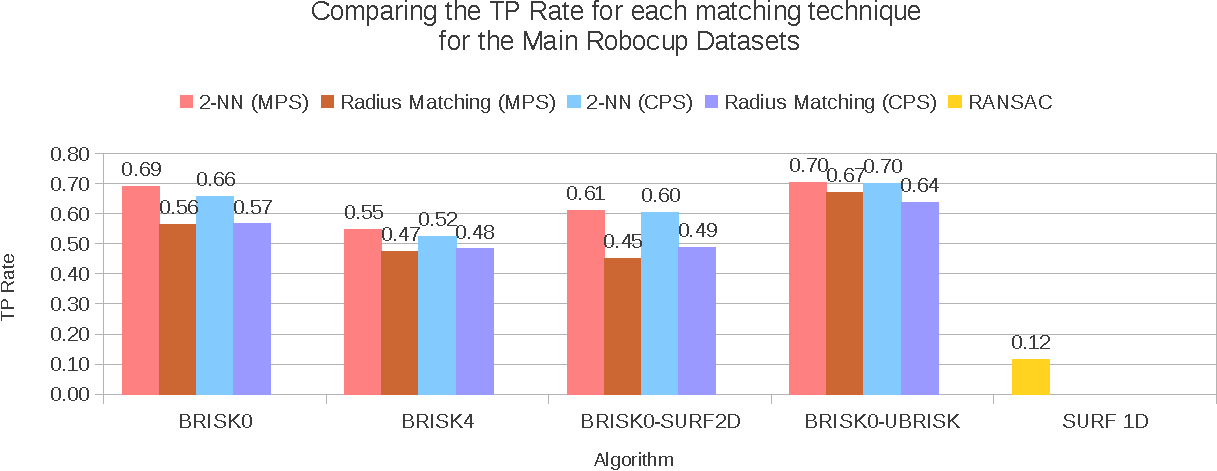
\includegraphics[width=1.0\textwidth]{../Drawings/Graphs/tp_rate_mrb.pdf}
    \caption{The $TP_{FP=0}^{max}$ rate for the Main Robocup datasets} 
    \label{fig:tp_rate_mrd}
\end{figure}

Based on the above results, BRISK0 - U-BRISK seems to produce the best overall performance. Since processing time is a crucial factor in determining which algorithm is best, the main candidates are BRISK0 - U-BRISK and 1D SURF. However, 1D SURF is not able to attain a large $TP_{FP=0}^{max}$ value in this environment. In order to verify that the BRISK0 - U-BRISK algorithm does indeed have better overall performance than the other feature extraction algorithms, the algorithms need to be tested in various different environments.\\ 

%This data was generated by considering overlapping and non-overlapping images
%The valid matches and invalid matches should differ between the matching and overlapping sets respectively.

%\begin{table}
%\caption{The matched point and keypoint statistics for the Main Robocup Datasets
%using 2-NN matching}
%\begin{tabular}{|c|c|c|c|c|}
%\hline 
%Method & Overlapping images &  &  & \tabularnewline
%\hline 
%\hline 
% & Total Matches & Valid Matches & Invalid Matches & Mean Num Interest Points\tabularnewline
%\hline 
%SBRISK  & 175.56 & 15.420 & 160.14 & 87.780\tabularnewline
%\hline 
%BRISK4 & 175.63 & 13.230 & 162.41 & 87.820\tabularnewline
%\hline 
%SBRISK-SURF2D  & 218.88 & 19.010 & 199.86 & 109.44\tabularnewline
%\hline 
%SBRISK - UBRISK & 135.76 & 16.140 & 119.62 & 67.880\tabularnewline
%\hline 
%1D SURF & 15.850 & 9.1000 & 6.7500 & 50.880\tabularnewline
%\hline 
% & Non-overlapping images &  &  & \tabularnewline
%\hline 
%SBRISK  & 72.260 & 0.25000 & 72.010 & 42.850\tabularnewline
%\hline 
%BRISK4  & 69.930 & 0.28000 & 69.640 & 41.530\tabularnewline
%\hline 
%SBRISK-SURF2D & 98.700 & 1.3900 & 97.310 & 56.840\tabularnewline
%\hline 
%SBRISK - UBRISK & 54.560 & 0.22000 & 54.340 & 32.610\tabularnewline
%\hline 
%1D SURF & 12.960 & 6.4800 & 6.4700 & 53.290\tabularnewline
%\hline 
%\end{tabular}
%\label{tab:mrdMKKnn}
%\end{table}

%\begin{table}
%\caption{The matched point and keypoint statistics for the Main Robocup Datasets
%using Radius Matching}
%\begin{tabular}{|c|c|c|c|c|}
%\hline 
%Method & Overlapping images &  &  & \tabularnewline
%\hline 
%\hline 
% & Total Matches & Valid Matches & Invalid Matches & Mean Num Interest Points\tabularnewline
%\hline 
%SBRISK  & 99.960 & 54.210 & 45.760 & 39.190\tabularnewline
%\hline 
%BRISK4 & 255.84 & 152.47 & 103.37 & 56.370\tabularnewline
%\hline 
%SBRISK-SURF2D  & 24.870 & 15.200 & 9.6600 & 68.990\tabularnewline
%\hline 
%SBRISK - UBRISK & 51.030 & 32.750 & 18.280 & 39.190\tabularnewline
%\hline 
%1D SURF & 15.850 & 9.1000 & 6.7500 & 50.880\tabularnewline
%\hline 
% & Non-overlapping images &  &  & \tabularnewline
%\hline 
%SBRISK  & 18.940 & 8.4400 & 10.490 & 17.020\tabularnewline
%\hline 
%BRISK4  & 30.530 & 14.260 & 16.280 & 22.550\tabularnewline
%\hline 
%SBRISK-SURF2D & 3.4900 & 1.1700 & 2.3200 & 34.920\tabularnewline
%\hline 
%SBRISK - UBRISK & 6.4100 & 2.9400 & 3.4700 & 17.020\tabularnewline
%\hline 
%1D SURF & 12.960 & 6.4800 & 6.4700 & 53.290\tabularnewline
%\hline 
%\end{tabular}
%\label{tab:mrdMKHamming}
%\end{table}

% \begin{figure}%[ht!]
%  \centering
%    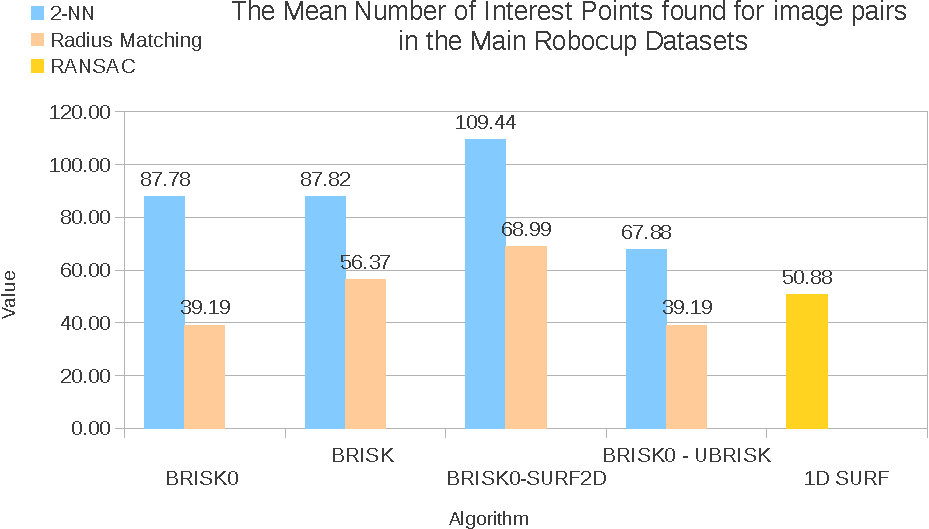
\includegraphics[width=1.0\textwidth]{../Drawings/Graphs/mrd_ip.pdf}
%    \caption{The mean number of interest points found for each matching technique in the Main Robocup datasets} 
%    \label{fig:mrd_ip}
% \end{figure}
% 
%\begin{figure}
%  \centering
%    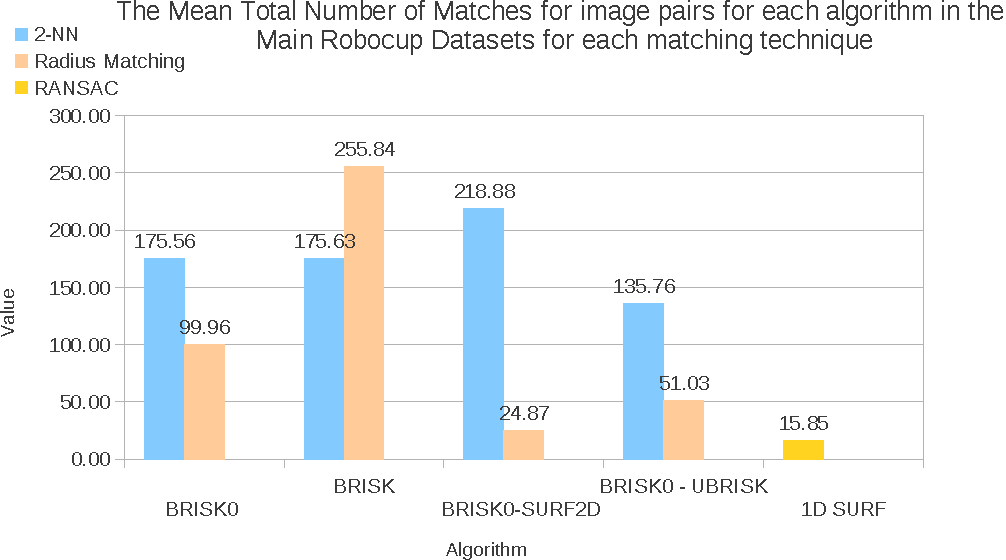
\includegraphics[width=1.0\textwidth]{../Drawings/Graphs/mrd_tnm.pdf}
%    \caption{The mean number total number of matches for each matching technique in the Main Robocup datasets} 
%    \label{fig:mrd_tnm}
%\end{figure}
%
%\begin{figure}
%  \centering
%    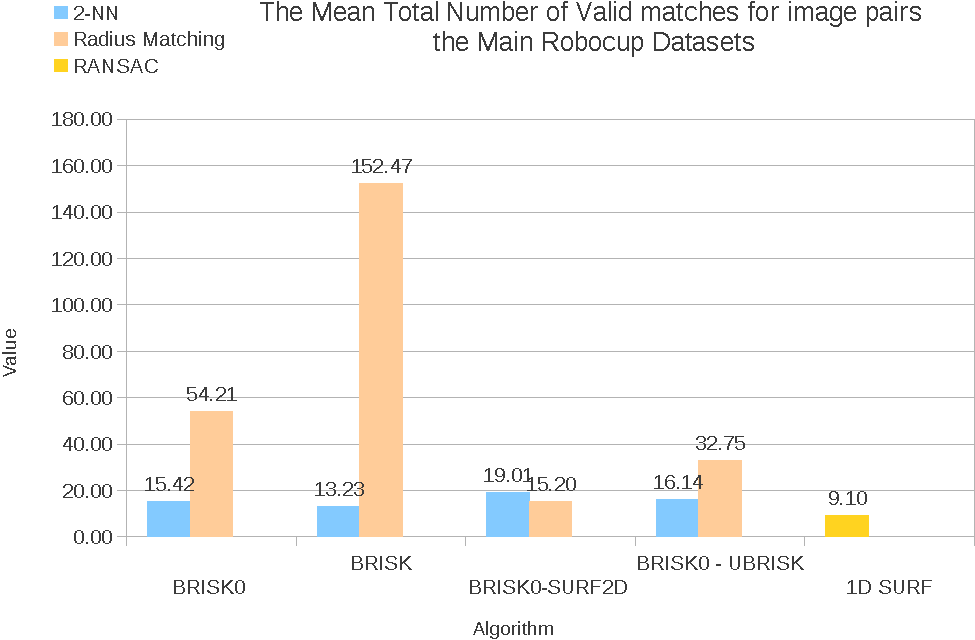
\includegraphics[width=1.0\textwidth]{../Drawings/Graphs/mrd_nvm.pdf}
%    \caption{The mean total number of valid matches for each matching technique in the Main Robocup datasets} 
%    \label{fig:mrd_nvm}
%\end{figure}

%\begin{figure}
%  \centering
%    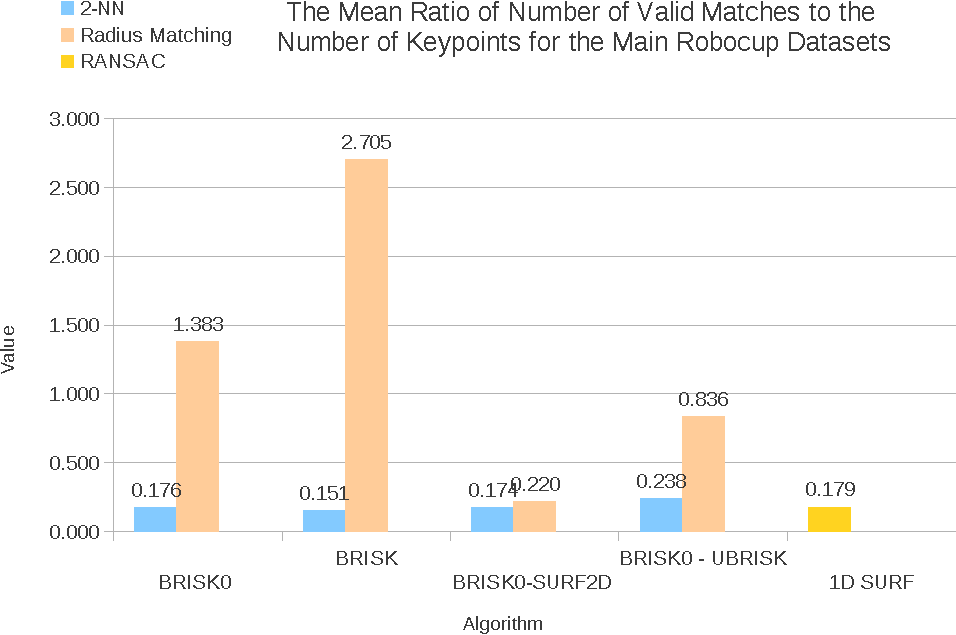
\includegraphics[width=1.0\textwidth]{../Drawings/Graphs/mrd_ratio.pdf}
%    \caption{The mean ratio of total number of valid matches to the total number of interest points detected for each matching technique in the Main Robocup datasets} 
%    \label{fig:mrd_ratio}
%\end{figure}

%\begin{figure}
%  \centering
%    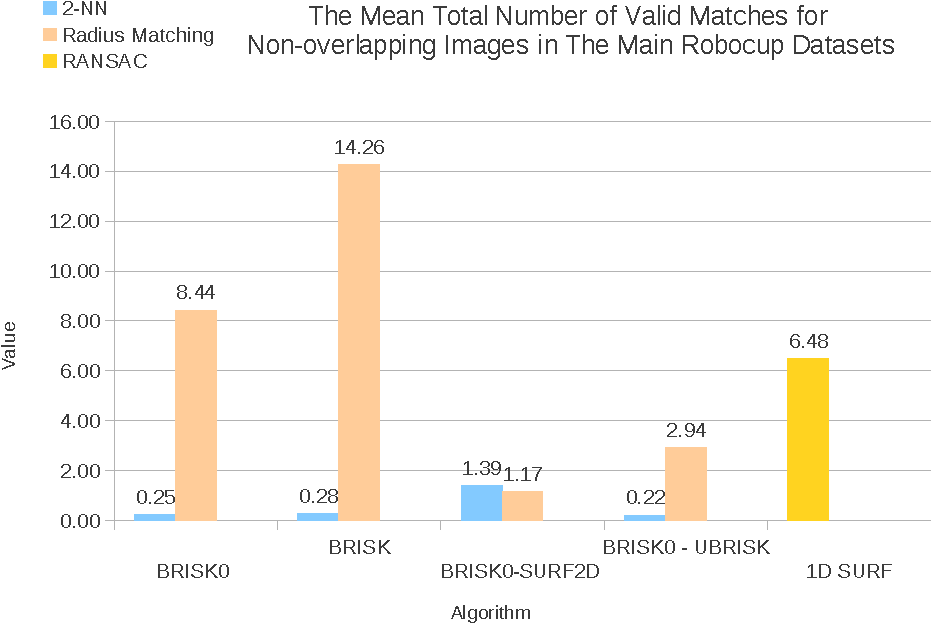
\includegraphics[width=1.0\textwidth]{../Drawings/Graphs/mrb_nvm_nol.pdf}
%    \caption{The number of mean valid matches detected for non-overlapping images in the Main Robocup datasets} 
%    \label{fig:mrd_nvm_nol}
%\end{figure}

%
% \begin{figure}%[ht!]
%  \centering
%    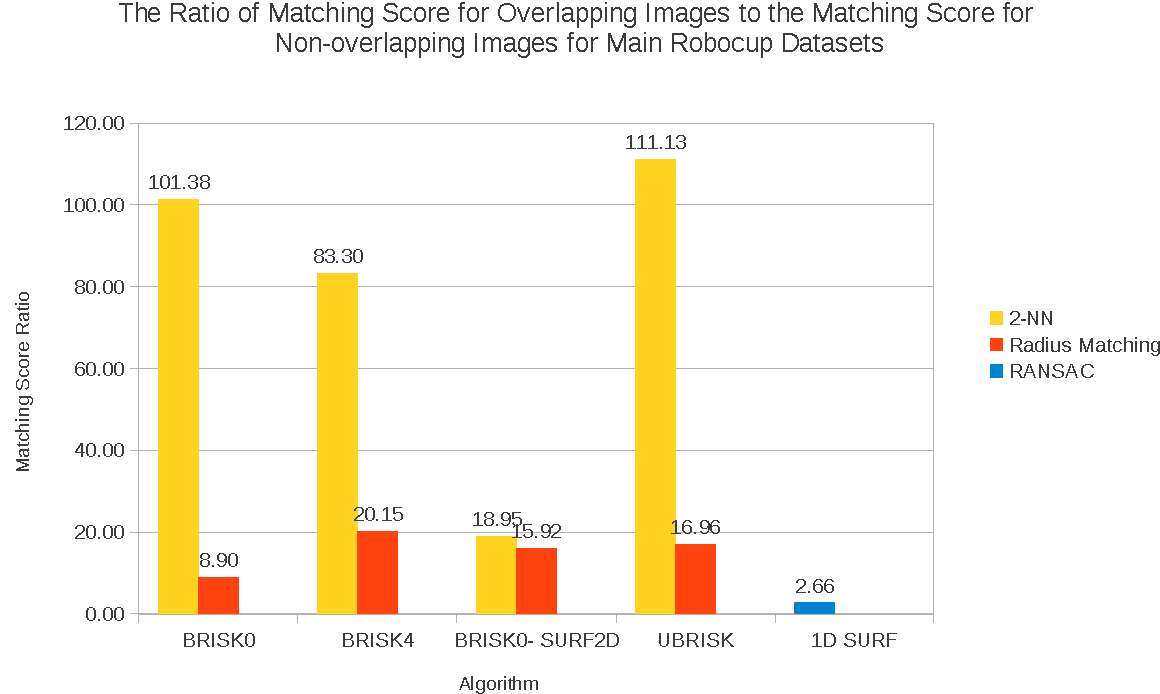
\includegraphics[width=1.0\textwidth]{../Drawings/Graphs/ms_ratio_mrd.pdf}
%    \caption{The Matching Score Ratio of the matching score of overlapping images to the matching score of non-overlapping images} 
%    \label{fig:ms_ratio_mrd}
% \end{figure}


%\begin{table}
%\caption{The thresholds at which the TP rate is a maximum whilst still maintaining
%a FP rate of 0 for each of the feature extraction algorithms. This
%is for 2-NN matching}
%\begin{tabular}{|c|c|c|}
%\hline 
%Method & Threshold & TP rate\tabularnewline
%\hline 
%\hline 
%BRISK0 & 0.0600 & 0.595\tabularnewline
%\hline 
%BRISK4 & 0.0500 & 0.572\tabularnewline
%\hline 
%BRISK0-SURF2D & 30 & 0.579\tabularnewline
%\hline 
%BRISK0-UBRISK & 0.0500 & 0.560\tabularnewline
%\hline 
%SURF 1D & 294 & 0.057\tabularnewline
%\hline 
%\end{tabular}
%\label{tab:tpRateRobocupKnn}
%\end{table}
%
%\begin{table}
%\caption{The thresholds at which the TP rate is a maximum whilst still maintaining
%a FP rate of 0 for each of the feature extraction algorithms. This
%is for Radius Matching}
%\begin{tabular}{|c|c|c|}
%\hline 
%Method & Threshold & TP rate\tabularnewline
%\hline 
%\hline 
%BRISK0 & 0.160 & 0.398\tabularnewline
%\hline 
%BRISK4 & 0.220 & 0.414\tabularnewline
%\hline 
%BRISK0-SURF2D & 32 & 0.465\tabularnewline
%\hline 
%BRISK0-UBRISK & 0.130 & 0.377\tabularnewline
%\hline 
%SURF 1D & 294 & 0.057\tabularnewline
%\hline 
%\end{tabular}
%\label{tab:tpRateRobocupHamming}
%\end{table}
\section{Performance in Additional Environments}
\label{sec:additionalDataset}
The first additional environment is a random office and the second environment is a large hall. The random office has been selected in order to add natural light into the scene from a large window and will be presented in \secref{sec:office}. It also has a large number of salient features that may improve or inhibit feature extraction performance. The large hall has been chosen such that the resolution of the images are lower since the Nao is observing features at large distances. This environment also has many salient features. \\

\subsection{Office Environment}
\label{sec:office}
Two datasets have been created from a random office environment. In total $25$ overlapping images from one side of the office correspond to one dataset and a further $25$ overlapping images from another view of the office correspond to a second dataset. These images have been taken at various scales and angles. Typical images from each viewpoint are shown in \figref{fig:dataset5} and \figref{fig:dataset6} respectively.\\


\begin{figure}[h!]
\begin{minipage}[b]{0.5\linewidth}
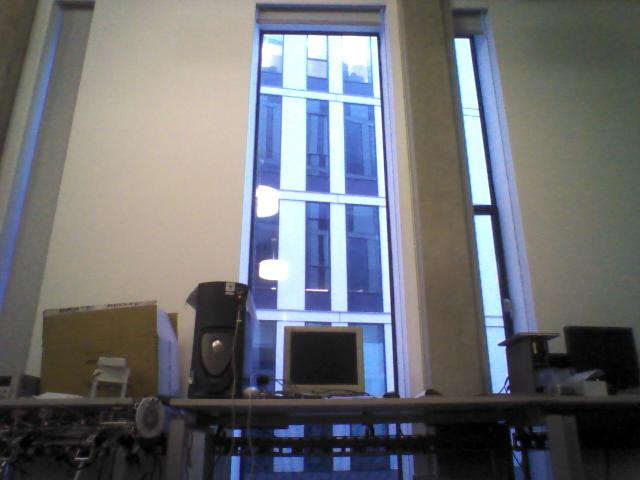
\includegraphics[scale=0.5]{../Drawings/datasetImages/dataset5.jpg}
\caption{The first dataset showing a typical image from one side of the random office environment}
\label{fig:dataset5}
\end{minipage}
\hspace{0.5cm}
\begin{minipage}[b]{0.5\linewidth}
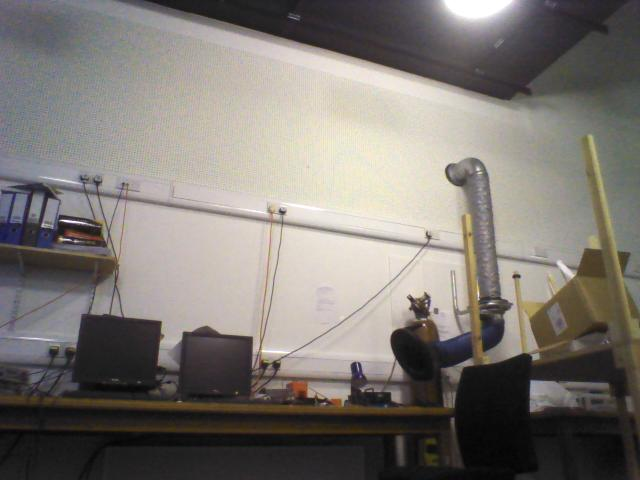
\includegraphics[scale=0.5]{../Drawings/datasetImages/dataset6.jpg}
\caption{The second dataset showing a typical image from one side of the random office environment}
\label{fig:dataset6}
\end{minipage}
\end{figure}

In total $600$ overlapping pairs of images and $600$ non-overlapping pairs of images were generated. Utilising the MPS values calculated in \secref{sec:optimalParameters}, the feature extraction algorithms were tested on each of the overlapping and non-overlapping image pairs. The feature extraction algorithms were tested using both the 2-NN matching and Radius Matching techniques respectively. The corresponding ROC curves generated from this data are displayed in \figref{fig:compareKnnOffice} and \figref{fig:compareHammingOffice}. The CPS statistics can be found in Appendix A, \secref{app:oe}. \\

\figref{fig:compareKnnOffice} and \figref{fig:compareHammingOffice} shows the ROC curves that were generated when using the MPS values and 2-NN and Radius Matching respectively. The statistics quantifying the computational performance as well as AUC values for each of the feature extraction algorithms are shown in \tabref{tab:oe_times_knn} and \tabref{tab:oe_times_hamming} for 2-NN and Radius Matching respectively. \\

An important observation from these image datasets is the fact that more interest points are found on average in the \textit{Office Environment} compared to the \textit{Main Robocup Environment} using each of the feature extraction algorithms. This is verified by analysing the graphs shown in \figref{fig:overall_tn_ip} and \figref{fig:overall_tn_ip_radius}. The reason more interest points are detected is based on the nature of the \textit{Office Environment}. There are salient features present in the \textit{Office Environment} such as the large window seen in \figref{fig:dataset5}. Features such as these have strong edges which generate interest points. Interest points are also detected in regions of high texture \cite{Szeliski2010}. An example of this is shown in \figref{fig:oe_interestPoints}. As can be seen in the figure, the edges of the windows have a large number of interest points. In addition to this, the bookshelf  in the right image also generates a large number of interest points due to the variation in texture. These salient image features tend to create strong interest points and this ultimately improves the performance in matching overlapping image pairs and rejecting non-overlapping image pairs. The natural light from the window is also partially responsible for generating stronger edges as a large number of interest points are detected in the window region as shown in \figref{fig:oe_interestPoints}. \\



\begin{figure}
  \centering
    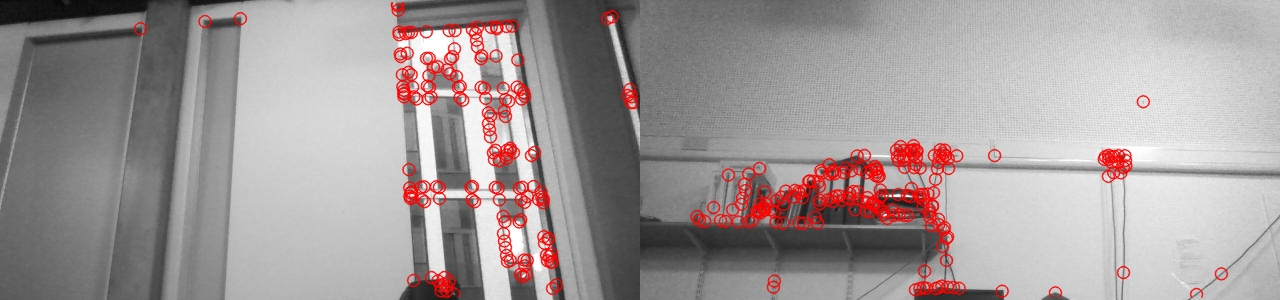
\includegraphics[width=1.0\textwidth]{../Drawings/Matching/dataset2_interestPoints.jpg}
    \caption{Typical interest points detected in the images from the \textit{Office Environment Datasets}} 
    \label{fig:oe_interestPoints}
\end{figure}


In addition to an increase in the number of interest points, the total number of matches found for 2-NN Matching have increased as expected as shown in \figref{fig:overall_tnm}. The total number of matches have increased for BRISK0-SURF2D, BRISK0 - U-BRISK and 1D SURF when using Radius Matching as shown in \figref{fig:overall_tnm_radius}. However, they have decreased for BRISK0 and BRISK. As mentioned in \secref{sec:mrdPerformance}, the large number of matches generated by these two algorithms in the \textit{Main Robocup Environment} were largely due to duplicate matches from the ceiling lights. The \textit{Office Environment} does not contain lighting that saturates the pixels as was the case in the \textit{Main Robocup Environment}. Thus, a decrease in the amount of detected interest points seems plausible.\\


Some important observations should be noted when analysing the computational performance of each of the feature extraction algorithms shown in \tabref{tab:oe_times_knn} and \tabref{tab:oe_times_hamming}. In general, there is an increase in the matching time for each of the algorithms using both 2-NN and Radius Matching since more matches are detected. In addition BRISK0 and BRISK have larger extraction times since rotating the sampling pattern for more interest points is a time consuming operation.\\

Less IZMs are generated as shown in \tabref{tab:oe_izm} for both matching techniques since more matches are detected due to the salient features in the \textit{Office Environment}. \\

As mentioned previously in \secref{sec:matchingScore}, the mean $IMS_{best}$ value between image pairs is generally much larger for overlapping images compared to non-overlapping images. However, the non-overlapping $IMS_{best}$ value is larger compared to the \textit{Main Robocup Environment} since more interest points are being matched in non-overlapping images. This may explain the slight decrease in AUC values seen in \tabref{tab:oe_times_knn} and \tabref{tab:oe_times_hamming} .\\

%The images are also taken in a setting of higher contrast.

%DISCUSS THAT THE HIGHEST TP MATCHING RATE AT WHICH THE FP RATE IS STILL 0, IS A GOOD INDICATOR OF PERFORMANCE.


\begin{figure}[h!]
\begin{minipage}[b]{0.5\linewidth}
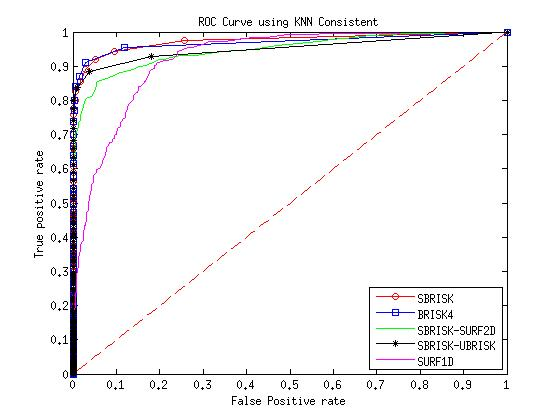
\includegraphics[scale=0.4]{../Drawings/dataset2_ROC_General_KNN.jpg}
\caption{A comparison of the ROC curves in the office environment using the MPS thresholds}
\label{fig:compareKnnOffice}
\end{minipage}
\hspace{0.5cm}
\begin{minipage}[b]{0.5\linewidth}
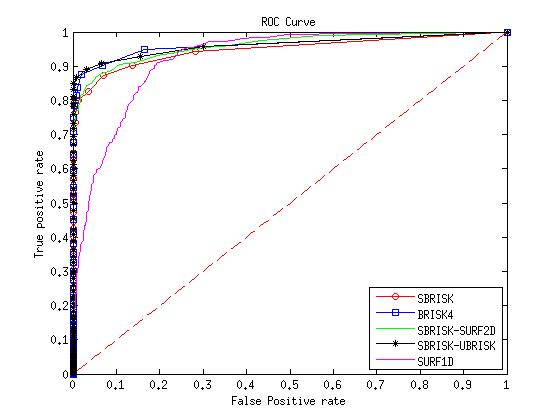
\includegraphics[scale=0.4]{../Drawings/dataset2_ROC_General_Hamming.jpg}
\caption{A comparison of the ROC curves in the office environment using the MPS Hamming/Euclidean distance thresholds}
\label{fig:compareHammingOffice}
\end{minipage}

\end{figure}



\begin{table}
\caption{The AUC and performance statistics for the office environment using
2-NN}
\footnotesize
\begin{tabular}{|c|c|c|c|c|c|c|c|}
\hline 
\textbf{Method (2-NN)} & \textbf{Parameters} & \textbf{\% AUC} & \textbf{Detection} & \textbf{Extraction} & \textbf{Matching} & \textbf{Verification} & \textbf{Overall}\tabularnewline
 &  &  & \textbf{Time (ms)} & \textbf{Time (ms)} & \textbf{Time (ms)} & \textbf{Time (ms)} & \textbf{Time (ms)}\tabularnewline
\hline 
\hline 
BRISK0 & MPS & 97.441 & 3.695 & 8.166 & 5.512 & 0.065 & 21.838\tabularnewline
\hline 
BRISK4 & MPS & 96.933 & 12.096 & 7.106 & 5.252 & 0.072 & 28.970\tabularnewline
\hline 
BRISK0-SURF2D & MPS & 94.795 & 3.793 & 17.157 & 1.497 & 0.083 & 26.936\tabularnewline
\hline 
\textbf{BRISK0-UBRISK} & \textbf{MPS} & \textbf{95.134} & \textbf{3.469} & \textbf{3.112} & \textbf{3.245} & \textbf{0.052} & \textbf{14.245}\tabularnewline
\hline 
\textbf{SURF 1D} & \textbf{Given} & \textbf{92.333} & \textbf{0.277} & \textbf{0.197} & \textbf{0.483} & \textbf{0.043} & \textbf{14.144}\tabularnewline
\hline 
\end{tabular}
\label{tab:oe_times_knn}
\end{table}

\begin{table}
\caption{The AUC and performance statistics for the office environment using
Radius Matching}
\footnotesize
\begin{tabular}{|c|c|c|c|c|c|c|c|}
\hline 
\textbf{Method (2-NN)} & \textbf{Parameters} & \textbf{\% AUC} & \textbf{Detection} & \textbf{Extraction} & \textbf{Matching} & \textbf{Verification} & \textbf{Overall}\tabularnewline
 & Some  &  & \textbf{Time (ms)} & \textbf{Time (ms)} & \textbf{Time (ms)} & \textbf{Time (ms)} & \textbf{Time (ms)}\tabularnewline
\hline 
\hline 
BRISK0 & MPS & 94.846 & 3.094 & 3.461 & 0.808 & 0.011 & 11.710\tabularnewline
\hline 
BRISK4 & MPS & 96.226 & 8.626 & 3.265 & 0.847 & 0.012 & 17.198\tabularnewline
\hline 
BRISK0-SURF2D & MPS & 96.054 & 3.255 & 8.495 & 0.489 & 0.019 & 16.626\tabularnewline
\hline 
\textbf{BRISK0-UBRISK} & \textbf{MPS} & \textbf{96.149} & \textbf{3.125} & \textbf{2.057} & \textbf{0.883} & \textbf{0.014} & \textbf{10.453}\tabularnewline
\hline 
\textbf{SURF 1D} & \textbf{Given} & \textbf{92.333} & \textbf{0.277} & \textbf{0.197} & \textbf{0.483} & \textbf{0.043} & \textbf{14.144}\tabularnewline
\hline 
\end{tabular}
\label{tab:oe_times_hamming}
\end{table}

%\begin{table}
%\caption{The matched point and keypoint statistics for the Office Environment
%Datasets using 2-NN matching}
%\begin{tabular}{|c|c|c|c|c|}
%\hline 
%Method  & Overlapping images &  &  & \tabularnewline
%\hline 
%\hline 
% & Total Matches & Valid Matches & Invalid Matches & Mean Num Interest Points\tabularnewline
%\hline 
%SBRISK  & 266.36 & 36.940 & 229.43 & 133.18\tabularnewline
%\hline 
%BRISK4 & 262.03 & 26.670 & 235.36 & 131.01\tabularnewline
%\hline 
%SBRISK-SURF2D  & 338.03 & 39.260 & 298.78 & 169.02\tabularnewline
%\hline 
%SBRISK - UBRISK & 202.14 & 32.570 & 169.58 & 101.07\tabularnewline
%\hline 
%1D SURF & 25.680 & 16 & 9.6900 & 69.430\tabularnewline
%\hline 
% & Non-overlapping images &  &  & \tabularnewline
%\hline 
%SBRISK  & 257.44 & 0.92000 & 256.52 & 131.22\tabularnewline
%\hline 
%BRISK4  & 324.24 & 0.64000 & 323.60 & 138.74\tabularnewline
%\hline 
%SBRISK-SURF2D & 317.28 & 6.4600 & 310.83 & 165.87\tabularnewline
%\hline 
%SBRISK - UBRISK & 207.68 & 0.72000 & 206.96 & 101.17\tabularnewline
%\hline 
%1D SURF & 11.690 & 5.9000 & 5.7900 & 70.930\tabularnewline
%\hline 
%\end{tabular}
%\label{tab:oeMKKnn}
%\end{table}
%
%\begin{table}
%\caption{The matched point and keypoint statistics for the Office Environment
%Datasets using Radius Matching}
%\begin{tabular}{|c|c|c|c|c|}
%\hline 
%Method & Overlapping images &  &  & \tabularnewline
%\hline 
%\hline 
% & Total Matches & Valid Matches & Invalid Matches & Mean Num Interest Points\tabularnewline
%\hline 
%SBRISK  & 27.720 & 20.090 & 7.6300 & 51.450\tabularnewline
%\hline 
%BRISK4 & 24.680 & 19.230 & 5.4500 & 51.870\tabularnewline
%\hline 
%SBRISK-SURF2D  & 52.610 & 35.400 & 17.210 & 84.430\tabularnewline
%\hline 
%SBRISK - UBRISK & 45.660 & 34.940 & 10.710 & 53.400\tabularnewline
%\hline 
%1D SURF & 25.680 & 16 & 9.6900 & 69.430\tabularnewline
%\hline 
% & Non-overlapping images &  &  & \tabularnewline
%\hline 
%SBRISK  & 1.8800 & 0.85000 & 1.0400 & 52.930\tabularnewline
%\hline 
%BRISK4  & 1.6700 & 0.89000 & 0.78000 & 58.720\tabularnewline
%\hline 
%SBRISK-SURF2D & 4.7400 & 1.5200 & 3.2200 & 85.830\tabularnewline
%\hline 
%SBRISK - UBRISK & 2.7500 & 1.2700 & 1.4800 & 55.140\tabularnewline
%\hline 
%1D SURF & 11.690 & 5.9000 & 5.7900 & 70.930\tabularnewline
%\hline 
%\end{tabular}
%\label{tab:oeMKHamming}
%\end{table}

%\begin{figure}%[ht!]
%  \centering
%    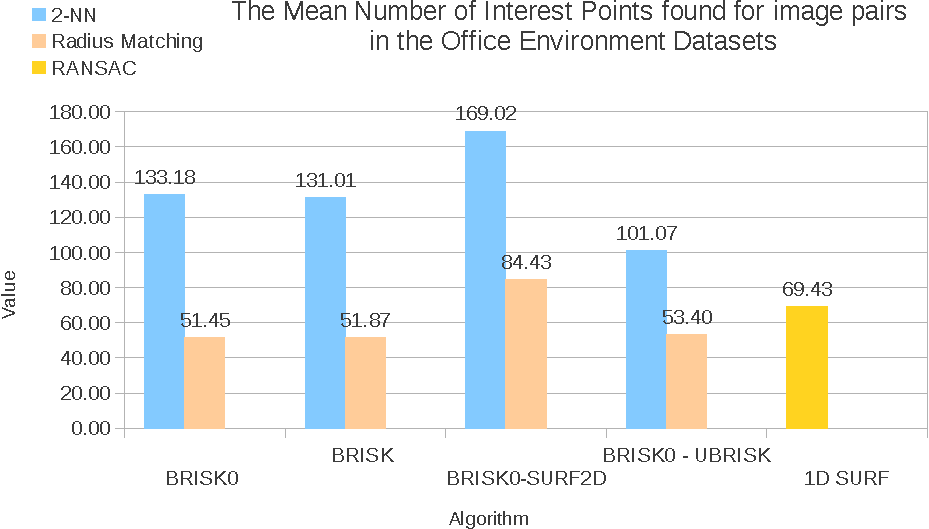
\includegraphics[width=1.0\textwidth]{../Drawings/Graphs/oe_ip.pdf}
%    \caption{The mean number of interest points found for each matching technique in the Office Environment datasets} 
%    \label{fig:oe_ip}
% \end{figure}
% 
%\begin{figure}
%  \centering
%    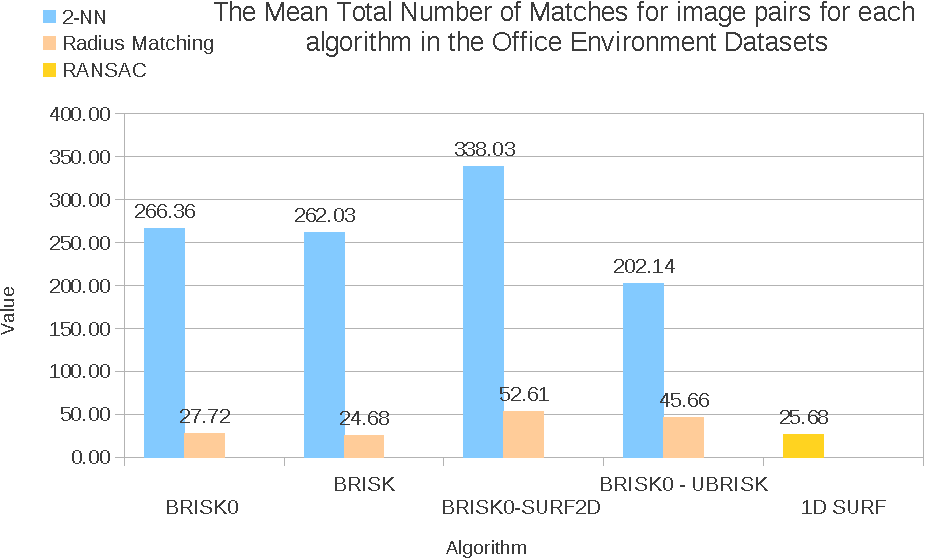
\includegraphics[width=1.0\textwidth]{../Drawings/Graphs/oe_tnm.pdf}
%    \caption{The mean number total number of matches for each matching technique in the Office Environment datasets} 
%    \label{fig:oe_tnm}
%\end{figure}
%
%\begin{figure}
%  \centering
%    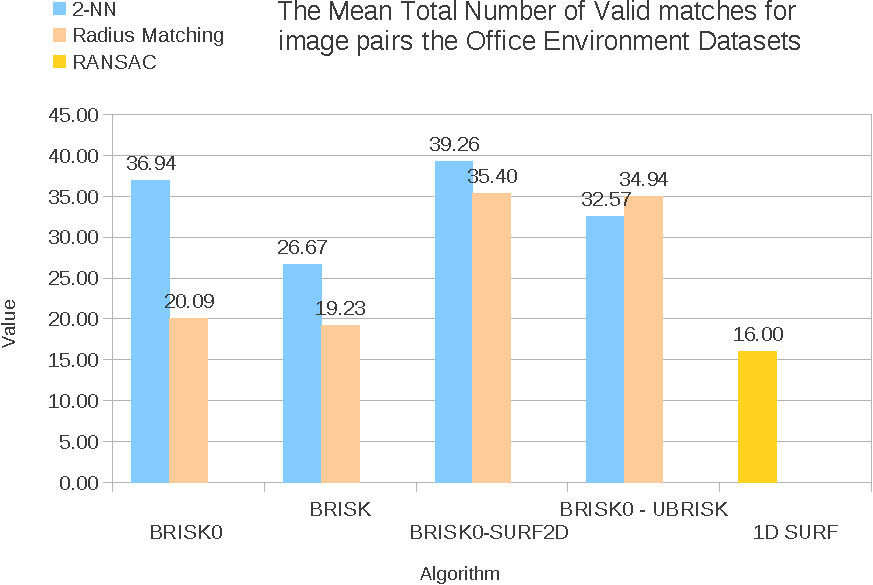
\includegraphics[width=1.0\textwidth]{../Drawings/Graphs/oe_nvm.pdf}
%    \caption{The mean total number of valid matches for each matching technique in the Office Environment datasets} 
%    \label{fig:oe_nvm}
%\end{figure}

%\begin{figure}
%  \centering
%    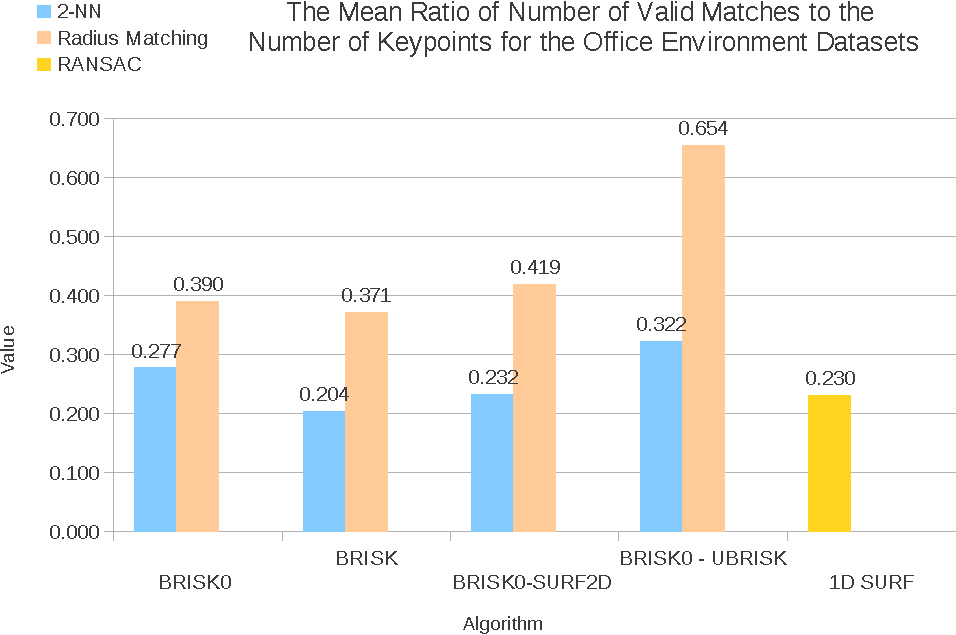
\includegraphics[width=1.0\textwidth]{../Drawings/Graphs/oe_ratio.pdf}
%    \caption{The mean ratio of total number of valid matches to the total number of interest points detected for each matching technique in the Office Environment datasets} 
%    \label{fig:oe_ratio}
%\end{figure}

%\begin{figure}
%  \centering
%    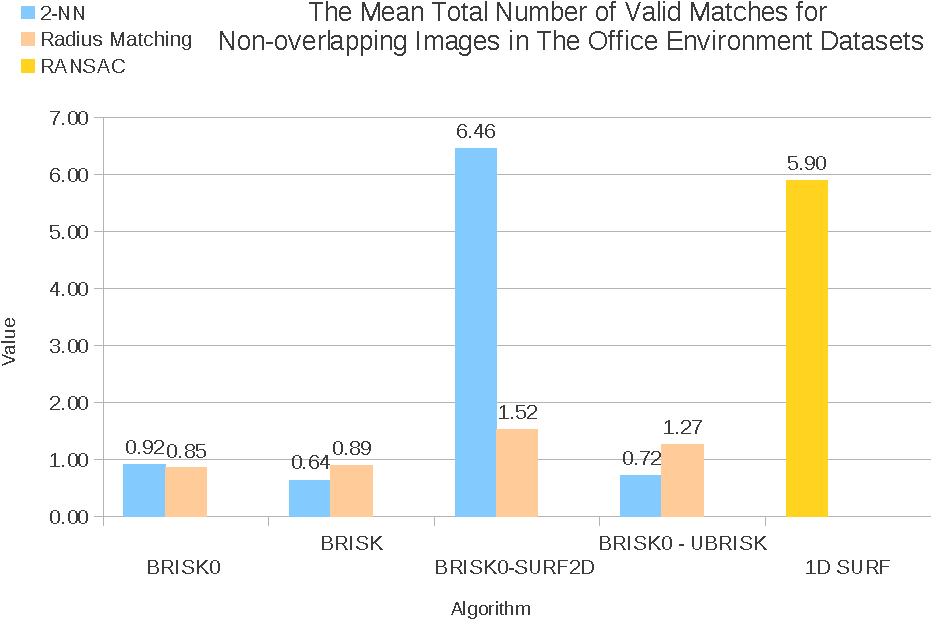
\includegraphics[width=1.0\textwidth]{../Drawings/Graphs/oe_nvm_nol.pdf}
%    \caption{The number of mean valid matches detected for non-overlapping images in the Office Environment datasets} 
%    \label{fig:oe_nvm_nol}
%\end{figure}

\begin{table}
\caption{The Number of Zero Matches (NZMs) for each feature extraction algorithm
using 2-NN and Radius Matching in the Office Environment}
\begin{tabular}{|c|c|}
\hline 
\textbf{Method} & \textbf{Number of Zero Matches}\tabularnewline
\hline 
 & \textbf{2-NN Matching}\tabularnewline
\hline 
\hline 
BRISK0 & 11.00\tabularnewline
\hline 
BRISK & 17.00\tabularnewline
\hline 
BRISK0- SURF2D & 0.00\tabularnewline
\hline 
UBRISK & 35.00\tabularnewline
\hline 
1D SURF & 0.00\tabularnewline
\hline 
 & \textbf{Radius Matching}\tabularnewline
\hline 
BRISK0 & 23.00\tabularnewline
\hline 
BRISK & 12.00\tabularnewline
\hline 
BRISK0- SURF2D & 7.00\tabularnewline
\hline 
UBRISK & 13.00\tabularnewline
\hline 
1D SURF & 0.00\tabularnewline
\hline 
\end{tabular}
\label{tab:oe_izm}
\end{table}



\begin{table}
\caption{The Matching Score for the Office Environment Dataset}
\begin{tabular}{|c|c|c|}
\hline 
\textbf{Method} & \textbf{Overlapping Score} & \textbf{Non-overlapping Score}\tabularnewline
\hline 
\hline 
 & \textbf{2-NN} & \tabularnewline
\hline 
\textbf{BRISK0} & 0.415 & 0.006\tabularnewline
\hline 
\textbf{BRISK4} & 0.263 & 0.004\tabularnewline
\hline 
\textbf{BRISK0- SURF2D} & 134.685 & 14.871\tabularnewline
\hline 
\textbf{UBRISK} & 0.321 & 0.004\tabularnewline
\hline 
\textbf{1D SURF} & 284.880 & 45.739\tabularnewline
\hline 
 & \textbf{Radius Matching} & \tabularnewline
\hline 
\textbf{BRISK0} & 0.228 & 0.008\tabularnewline
\hline 
\textbf{BRISK4} & 0.185 & 0.006\tabularnewline
\hline 
\textbf{BRISK0- SURF2D} & 115.377 & 5.832\tabularnewline
\hline 
\textbf{UBRISK} & 0.290 & 0.010\tabularnewline
\hline 
\textbf{1D SURF} & 284.880 & 45.739\tabularnewline
\hline 
\end{tabular}
\label{tab:oeMS}
\end{table}

% \begin{figure}%[ht!]
%  \centering
%    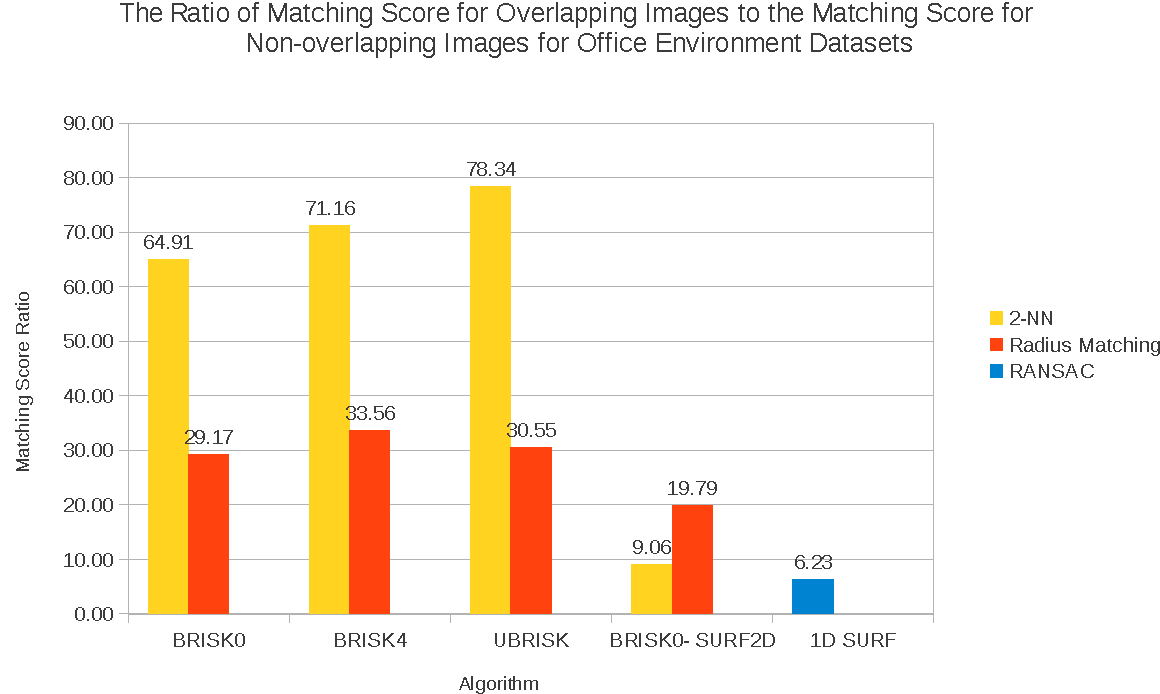
\includegraphics[width=1.0\textwidth]{../Drawings/Graphs/ms_ratio_oe.pdf}
%    \caption{The Matching Score Ratio of the matching score of overlapping images to the matching score of non-overlapping images for the Office Environment Datasets} 
%    \label{fig:ms_ratio_oe}
% \end{figure}



From the results shown in \figref{tp_rate_oe} for 2-NN and Radius Matching respectively, it can be seen that the $TP_{FP=0}^{max}$ value for each of the methods has increased. This is mainly due to the variation in the images creating a large number of strong salient interest points which has been shown previously to improve matching performance.\\

A notable increase in the $TP_{FP=0}^{max}$ value to $0.81$ is achieved for the BRISK0 - U-BRISK algorithm when using Radius Matching. A larger mean $IMS_{best}$ value compared to the \textit{Main Robocup Environment} is a central factor in generating this statistic. This causes more overlapping image pairs to be matched at higher $IMS_{best}$ thresholds. This has the effect of increasing the TP rate faster whilst maintaining a zero FP rate yielding a higher $TP_{FP=0}^{max}$ value.\\


%\begin{table}
%\caption{The thresholds at which the TP rate is a maximum whilst still maintaining
%a FP rate of 0 for each of the feature extraction algorithms. This
%is for 2-NN of the Office Environment}
%\begin{tabular}{|c|c|c|}
%\hline 
%Method & Threshold & TP rate\tabularnewline
%\hline 
%\hline 
%BRISK0 & 0.090 & 0.758\tabularnewline
%\hline 
%BRISK4 & 0.070 & 0.738\tabularnewline
%\hline 
%BRISK0-SURF2D & 79 & 0.585\tabularnewline
%\hline 
%BRISK0-UBRISK & 0.10 & 0.633\tabularnewline
%\hline 
%SURF 1D & 432 & 0.180\tabularnewline
%\hline 
%\end{tabular}
%\label{tab:tpRocOfficeKnn}
%\end{table}
%
%\begin{table}
%\caption{The thresholds at which the TP rate is a maximum whilst still maintaining
%a FP rate of 0 for each of the feature extraction algorithms. This
%is for Radius Matching of the Office Environment}
%\begin{tabular}{|c|c|c|}
%\hline 
%Method & Threshold & TP rate\tabularnewline
%\hline 
%\hline 
%BRISK0 & 0.080 & 0.718\tabularnewline
%\hline 
%BRISK4 & 0.080 & 0.71\tabularnewline
%\hline 
%BRISK0-SURF2D & 54 & 0.682\tabularnewline
%\hline 
%BRISK0-UBRISK & 0.080 & 0.81\tabularnewline
%\hline 
%SURF 1D & 432 & 0.18\tabularnewline
%\hline 
%\end{tabular}
%\label{tpRocOfficeHamming}
%\end{table}

\begin{figure}
  \centering
    \includegraphics[width=1.0\textwidth]{../Drawings/Graphs/tp_rate_oe.pdf}
    \caption{The mean ratio of total number of valid matches to the total number of interest points detected for each matching technique in the Office Environment datasets} 
    \label{fig:tp_rate_oe}
\end{figure}

As can be seen in the \textit{Office Environment}, BRISK0 - U-BRISK has the best timing of the BRISK-based techniques achieving a mean overall time of $10.45 ms$ in the best case when using Radius Matching. It also maintains a comparably good AUC value and has the largest $TP_{FP=0}^{max}$ value of all the algorithms.\\  

The 1D SURF implementation has also improved upon its performance as expected due an increase in the amount of salient features in the dataset images. The algorithm is able to better discriminate the features, detecting stronger interest points, and subsequently generate a larger AUC value. In addition to this improvement, the algorithm still maintains its speed and produces the fastest feature detection and matching performance as seen in \tabref{tab:oe_times_knn} and \tabref{tab:oe_times_hamming}. However, the $TP_{FP=0}^{max}$ value still suffers due to the comparably large $IMS_{best}$ score for non-overlapping images. This causes FPs to be generated at higher $IMS_{best}$ thresholds yielding the low $TP_{FP=0}^{max}$ value of $0.18$. \\


\subsection{Large Hall Environment}
\label{sec:largeHall}
The second environment, as mentioned previously, has been generated in a large hall. Two more datasets were created for this environment, with each dataset containing $15$ images from a particular side of the hall. Typical images from these datasets can be seen in \figref{fig:largeHall1} and \figref{fig:largeHall2} respectively.\\ 

\begin{figure}[h!]
\begin{minipage}[b]{0.5\linewidth}
\includegraphics[scale=0.5]{../Drawings/datasetImages/dataset3_1.jpg}
\caption{A typical image from the first large hall dataset}
\label{fig:largeHall1}
\end{minipage}
\hspace{0.5cm}
\begin{minipage}[b]{0.5\linewidth}
\includegraphics[scale=0.5]{../Drawings/datasetImages/dataset3_2.jpg}
\caption{A typical image from the second large hall dataset}
\label{fig:largeHall2}
\end{minipage}
\end{figure}

Again, all five of the feature extraction techniques have been tested on overlapping and non-overlapping images. In this case there are $210$ overlapping image pairs and $210$ non-overlapping image pairs. The ROC curves generated from this experiment are shown in \figref{fig:compareKnnOffice3} and \figref{fig:compareHammingOffice3}. The statistics quantifying these ROC curves are shown in \tabref{tab:lh_times_knn} and \tabref{tab:lh_times_hamming} respectively.\\

\begin{figure}[h!]
\begin{minipage}[b]{0.5\linewidth}
\includegraphics[scale=0.4]{../Drawings/dataset3_ROC_General_KNN.jpg}
\caption{A comparison of the ROC curves in the large hall environment using the MPS thresholds}
\label{fig:compareKnnOffice3}
\end{minipage}
\hspace{0.5cm}
\begin{minipage}[b]{0.5\linewidth}
\includegraphics[scale=0.4]{../Drawings/dataset3_ROC_General_Hamming.jpg}
\caption{A comparison of the ROC curves in the large hall environment using the MPS Hamming/Euclidean distance thresholds}
\label{fig:compareHammingOffice3}
\end{minipage}
\end{figure}

\begin{table}
\caption{The AUC and performance statistics for the large hall environment
using 2-NN}
\footnotesize
\begin{tabular}{|c|c|c|c|c|c|c|c|}
\hline 
\textbf{Method (2-NN)} & \textbf{Parameters} & \textbf{\% AUC} & \textbf{Detection} & \textbf{Extraction} & \textbf{Matching} & \textbf{Verification} & \textbf{Overall}\tabularnewline
 &  &  & \textbf{Time (ms)} & \textbf{Time (ms)} & \textbf{Time (ms)} & \textbf{Time (ms)} & \textbf{Time (ms)}\tabularnewline
\hline 
\hline 
BRISK0 & MPS & 99.263 & 4.027 & 10.752 & 18.175 & 0.147 & 37.513\tabularnewline
\hline 
BRISK4 & MPS & 96.444 & 15.664 & 9.691 & 13.698 & 0.126 & 43.645\tabularnewline
\hline 
BRISK0-SURF2D & MPS & 95.697 & 4.208 & 22.242 & 4.241 & 0.188 & 35.389\tabularnewline
\hline 
\textbf{BRISK0-UBRISK} & \textbf{MPS} & \textbf{97.430} & \textbf{3.701} & \textbf{3.804} & \textbf{9.849} & \textbf{0.109} & \textbf{21.885}\tabularnewline
\hline 
\textbf{SURF 1D} & \textbf{Given} & \textbf{90.836} & \textbf{0.273} & \textbf{0.161} & \textbf{0.351} & \textbf{0.044} & \textbf{14.032}\tabularnewline
\hline 
\end{tabular}
\label{tab:lh_times_knn}
\end{table}


\begin{table}
\caption{The AUC and performance statistics for the Large Hall Environment
using Radius Matching}
\footnotesize
\begin{tabular}{|c|c|c|c|c|c|c|c|}
\hline 
\textbf{Method} & \textbf{Parameters} & \textbf{\% AUC} & \textbf{Detection} & \textbf{Extraction} & \textbf{Matching} & \textbf{Verification} & \textbf{Overall}\tabularnewline
 &  &  & \textbf{Time (ms)} & \textbf{Time (ms)} & \textbf{Time (ms)} & \textbf{Time (ms)} & \textbf{Time (ms)}\tabularnewline
\hline 
\hline 
BRISK0 & MPS & 96.739 & 3.233 & 4.565 & 2.321 & 0.021 & 14.642\tabularnewline
\hline 
BRISK4 & MPS & 95.516 & 10.115 & 3.952 & 1.341 & 0.017 & 19.893\tabularnewline
\hline 
BRISK0-SURF2D & MPS & 98.803 & 3.436 & 11.197 & 1.260 & 0.039 & 20.345\tabularnewline
\hline 
\textbf{BRISK0-UBRISK} & \textbf{MPS} & \textbf{93.150} & \textbf{3.249} & \textbf{2.516} & \textbf{2.614} & \textbf{0.026} & \textbf{12.824}\tabularnewline
\hline 
\textbf{SURF 1D} & \textbf{Given} & \textbf{90.836} & \textbf{0.273} & \textbf{0.161} & \textbf{0.351} & \textbf{0.044} & \textbf{14.032}\tabularnewline
\hline 
\end{tabular}
\label{tab:lh_times_hamming}
\end{table}

The first important statistic to note is that the number of interest points for both 2-NN and Radius Matching have increased considerably for all of the BRISK and 2D SURF-based techniques as seen in \figref{fig:overall_tnm} and \figref{fig:overall_tnm_radius}. This can again be explained by the increased texture in the images found in these datasets. This causes a comparably large number of interest points to be detected as can be seen in \figref{fig:lh_ip}. However, as can be seen in the right image, since features such as lights have been captured at a lower resolution due to distance, less interest points have been detected in these regions. Thus it seems that distance, and hence image resolution, effects the number of interest points that are detected.\\

1D SURF maintains a similar number of interest points. This is due to the nature of the algorithm whereby 1D SURF has been stated to detect on average $50$ to $70$ features \cite{Anderson}.\\


\begin{figure}
  \centering
    \includegraphics[width=1.0\textwidth]{../Drawings/Matching/dataset3_interestPoints.jpg}
    \caption{Typical interest points detected in the \textit{Large Hall Environment}} 
    \label{fig:lh_ip}
\end{figure}


In addition, the total number of matches and the total number of valid matches, shown in \figref{fig:overall_tnm} and \figref{fig:overall_nvm}, increase as expected for the BRISK and 2D-SURF based algorithms.\\

The matching times and extraction times increase for the respective algorithms as in the \textit{Office Environment} due to an increase in the number of detected interest points and total matches. There are far fewer IZMs for each of the algorithms as can be seen in \tabref{tab:lh_izm}. In addition to this, the overlapping $IMS_{best}$ value has increased for each of the BRISK and 2D SURF-based algorithms. Both these statistics result in the increased AUC values seen in \tabref{tab:lh_times_knn} and \tabref{tab:lh_times_hamming}. \\



\begin{table}
\caption{The Number of Zero Matches (NZMs) for each feature extraction algorithm
using 2-NN and Radius Matching in the Large Environment}
\begin{tabular}{|c|c|}
\hline 
\textbf{Method} & \textbf{Number of Zero Matches}\tabularnewline
\hline 
 & \textbf{2-NN Matching}\tabularnewline
\hline 
\hline 
BRISK0 & 0.00\tabularnewline
\hline 
BRISK & 5.00\tabularnewline
\hline 
BRISK0- SURF2D & 0.00\tabularnewline
\hline 
UBRISK & 0.00\tabularnewline
\hline 
1D SURF & 0.00\tabularnewline
\hline 
 & \textbf{Radius Matching}\tabularnewline
\hline 
BRISK0 & 0.00\tabularnewline
\hline 
BRISK & 0.00\tabularnewline
\hline 
BRISK0- SURF2D & 0.00\tabularnewline
\hline 
UBRISK & 3.00\tabularnewline
\hline 
1D SURF & 0.00\tabularnewline
\hline 
\end{tabular}
\label{tab:lh_izm}
\end{table}

\begin{table}
\caption{The Matching Score for the Large Hall Datasets}
\begin{tabular}{|c|c|c|}
\hline 
\textbf{Method} & \textbf{Overlapping Score} & \textbf{Non-overlapping Score}\tabularnewline
\hline 
\hline 
 & \textbf{2-NN} & \tabularnewline
\hline 
\textbf{BRISK0} & 2.354 & 0.010\tabularnewline
\hline 
\textbf{BRISK4} & 1.308 & 0.009\tabularnewline
\hline 
\textbf{BRISK0- SURF2D} & 568.871 & 24.824\tabularnewline
\hline 
\textbf{UBRISK} & 1.501 & 0.009\tabularnewline
\hline 
\textbf{1D SURF} & 136.433 & 32.639\tabularnewline
\hline 
 & \textbf{Radius Matching} & \tabularnewline
\hline 
\textbf{BRISK0} & 1.035 & 0.027\tabularnewline
\hline 
\textbf{BRISK4} & 0.484 & 0.022\tabularnewline
\hline 
\textbf{BRISK0- SURF2D} & 407.774 & 20.708\tabularnewline
\hline 
\textbf{UBRISK} & 1.014 & 0.027\tabularnewline
\hline 
\textbf{1D SURF} & 136.433 & 32.639\tabularnewline
\hline 
\end{tabular}
\label{tab:lhMS}
\end{table}

% \begin{figure}%[ht!]
%  \centering
%    \includegraphics[width=1.0\textwidth]{../Drawings/Graphs/ms_ratio_lh.pdf}
%    \caption{The Matching Score Ratio of the matching score of overlapping images to the matching score of non-overlapping images for the Large Hall Environment Datasets} 
%    \label{fig:ms_ratio_mrd}
% \end{figure}

There has also been an increase in the $TP_{FP=0}^{max}$ value as shown in \figref{fig:tp_rate_lh}. The best performance is achieved in this environment with BRISK0 generating the largest $TP_{FP=0}^{max}$ value of $0.92$ using 2-NN Matching. BRISK0 - U-BRISK has comparably good performance attaining a best case $TP_{FP=0}^{max}$ value of $0.90$ when utilising Radius Matching. 1D SURF has also increased its $TP_{FP=0}^{max}$ value to $0.60$ which is its highest of all the environments. This seems to indicate that 1D SURF relies on a textured environment to detect a sufficient number of discriminative, unambiguous interest points.\\

In general, from the above three environments a trend can be seen whereby many salient features resulting from textured environments increase the number of interest points that are detected. This seems to increase the number of total and valid matches respectively. This reduces the number of IZMs and increases the $IMS_{best}$ values resulting in improved $TP_{FP=0}^{max}$ values.\\

\begin{figure}
  \centering
    \includegraphics[width=1.0\textwidth]{../Drawings/Graphs/tp_rate_lh.pdf}
    \caption{The $TP_{FP=0}$ Rate for the Large Hall Environment datasets} 
    \label{fig:tp_rate_lh}
\end{figure}


Therefore, based on the above data, the BRISK0- U-BRISK algorithm using \textit{RadiusMatch} matching technique seems to produce the best overall performance and should therefore be implemented on the robot. Since it can perform image processing and feature extraction in a best case time of $8.81 ms$, it should be possible to use this method in real-time on the robot to perform the matching routine and ultimately help the robot disambiguate its position on the field.\\

\section{Matching Score Boundary}
\label{sec:matchingScoreBoundary}
In order to effectively utilise this method on the robot, a $IMS_{best}$ boundary, $IMS_{boundary}$, needs to be determined. When comparing a pair of images, if the matching score is above the $IMS_{boundary}$, then the images are considered to be overlapping and are marked as a match. If the matching score is below the $IMS_{boundary}$ then the images are not matched. \\

The $IMS_{boundary}$ needs to be defined such that no False Positives (FP) will be generated when matching two non-overlapping images. In order to implement this constraint, the $IMS_{best}$ threshold corresponding to the worst case $TP_{FP=0}^{max}$ value will be chosen as the $IMS_{boundary}$. The worst case $TP_{FP=0}^{max}$ resulted from the \textit{Main Robocup Testing Datasets} in the \textit{Main Robocup Environment}. An $IMS_{boundary}$ of $0.08$ has been chosen which produces a worst-case $TP_{FP=0}^{max}$ value of $0.67$. This means that approximately $2$ out of every $3$ overlapping images will be correctly classified as a TP. This is acceptable performance since, according to Aldebaran's documentation, the Nao's camera takes $30$ frames per second and will therefore process a large number of frames in a short period of time. Therefore if the Nao cannot find a match between a pair of images, it will subsequently have another $30$ images every second with which it can try and identify a matching pair.\\

\section{Lighting Variation}
\label{sec:lighting}
Since BRISK - U-BRISK using Radius Matching has been chosen as the feature extraction algorithm to be implemented on the Nao, various properties of the algorithm should be tested. This includes testing the robustness of the algorithm to changes in illumination. This is important because Robocup venues change every year and the illumination is almost certainly not uniform. In order to determine how well BRISK0 - U-BRISK performs in these conditions, three scenarios were created with slightly different lighting conditions. All of these scenarios were created in the \textit{Main Robocup Environment}, detailed in \secref{sec:datasets}.\\ 

For each scenario $i$ four image datasets were generated as in \secref{sec:datasets}. These include  two datasets of images behind the player's goal namely, \textit{$PG Left_{i}$} and \textit{$PG Right_i$} as well as two datasets behind the opponent's goal, namely \textit{$OG Left_i$} and \textit{$OG Right_i$} respectively. Each image dataset contains $15$ images. All of the images in each dataset were taken at the same scale since only the performance under varying illumination is being tested in this experiment.\\ 

The lighting setup in the Robocup test environment is as follows. The environment contains \textit{Main Lights} that are responsible for providing soft lighting to the room. In addition to these lights are two adjacent \textit{Fluorescent Lights} on the ceiling denoted \textit{Left Fluorescent Light} and \textit{Right Fluorescent Light}. Each fluorescent light stretches the length of the room and provides harder lighting than the main lights to the scene. \\

\textbf{ANM IMAGE OF THE LIGHTING SETUP IN THE ENVIRONMENT}

Scenario $1$ involves switching off only the \textit{Left Fluorescent Light} located on the ceiling. Typical images from each dataset generated in this scenario are shown in \figref{fig:leftmgleft} to \figref{fig:leftogright} respectively. Scenario $2$ involves turning off only the \textit{Right Fluorescent Light} located on the ceiling as well as the \textit{Main Lights}. Typical images from these datasets are shown in \figref{fig:rightmgleft} to \figref{fig:rightogright} respectively. Scenario $3$ involves turning off both the \textit{Left Fluorescent Light} and \textit{Right Fluorescent Light}, leaving only the \textit{Main Lights} on in the environment. Typical images from these datasets are shown in \figref{fig:bothmgleft} to \figref{fig:bothogright} respectively. It should be noted that scenario $3$ has the lowest illumination compared to the other two scenarios. \\

Each of the datasets from the three scenarios have been matched with the images from the \textit{Main Robocup Datasets} detailed in \secref{sec:datasets}. This means that, for example, \textit{$PG Left_1$} from scenario $1$ will be matched to \textit{PG Left} from the \textit{Main Robocup Datasets} and so on. These datasets are being compared in order to determine whether or not the BRISK0 - U-BRISK algorithm is robust to variations in illumination. The datasets have been matched as shown in \tabref{tab:datasetLighting} to produce $5040$ pairs of overlapping images and $10008$ pairs of non-overlapping images under varying lighting conditions.\\

\begin{figure}
\begin{minipage}[b]{0.5\linewidth}
\includegraphics[scale=0.3]{../Drawings/lighting/leftLight/1.jpg}
\caption{The area behind the player's goal to the left}
\label{fig:leftmgleft}
\end{minipage}
\hspace{0.5cm}
\begin{minipage}[b]{0.5\linewidth}
\includegraphics[scale=0.3]{../Drawings/lighting/leftLight/2.jpg}
\caption{The area behind the player's goal to the right}
\label{fig:leftmgright}
\end{minipage}
\begin{minipage}[b]{0.5\linewidth}
\includegraphics[scale=0.3]{../Drawings/lighting/leftLight/3.jpg}
\caption{The area behind the opponent's goal to the left}
\label{fig:leftogleft}
\end{minipage}
\hspace{0.5cm}
\begin{minipage}[b]{0.5\linewidth}
\includegraphics[scale=0.3]{../Drawings/lighting/leftLight/4.jpg}
\caption{The area behind the opponents goal to the right}
\label{fig:leftogright}
\end{minipage}
\caption{Typical images from the first illumination scenario where only a single light is turned off}
\end{figure}



\begin{figure}
\begin{minipage}[b]{0.5\linewidth}
\includegraphics[scale=0.3]{../Drawings/lighting/rightLight/1.jpg}
\caption{The area behind the player's goal to the left}
\label{fig:rightmgleft}
\end{minipage}
\hspace{0.5cm}
\begin{minipage}[b]{0.5\linewidth}
\includegraphics[scale=0.3]{../Drawings/lighting/rightLight/2.jpg}
\caption{The area behind the player's goal to the right}
\label{fig:rightmgright}
\end{minipage}
\begin{minipage}[b]{0.5\linewidth}
\includegraphics[scale=0.3]{../Drawings/lighting/rightLight/3.jpg}
\caption{The area behind the opponent's goal to the left}
\label{fig:rightogleft}
\end{minipage}
\hspace{0.5cm}
\begin{minipage}[b]{0.5\linewidth}
\includegraphics[scale=0.3]{../Drawings/lighting/rightLight/4.jpg}
\caption{The area behind the opponents goal to the right}
\label{fig:rightogright}
\end{minipage}
\caption{Typical images from the second illumination scenario where a single fluorescent light as well as the main lighting is turned off.}
\end{figure}



\begin{figure}
\begin{minipage}[b]{0.5\linewidth}
\includegraphics[scale=0.3]{../Drawings/lighting/bothLights/1.jpg}
\caption{The area behind the player's goal to the left}
\label{fig:bothmgleft}
\end{minipage}
\hspace{0.5cm}
\begin{minipage}[b]{0.5\linewidth}
\includegraphics[scale=0.3]{../Drawings/lighting/bothLights/2.jpg}
\caption{The area behind the player's goal to the right}
\label{fig:bothmgright}
\end{minipage}
\begin{minipage}[b]{0.5\linewidth}
\includegraphics[scale=0.3]{../Drawings/lighting/bothLights/3.jpg}
\caption{The area behind the opponent's goal to the left}
\label{fig:bothogleft}
\end{minipage}
\hspace{0.5cm}
\begin{minipage}[b]{0.5\linewidth}
\includegraphics[scale=0.3]{../Drawings/lighting/bothLights/4.jpg}
\caption{The area behind the opponents goal to the right}
\label{fig:bothogright}
\end{minipage}
\caption{Typical images from the third illumination scenario where a both fluorescent lights are turned off.}
\end{figure}


\begin{table}
\caption{The datasets that have been compared under varying lighting conditions
to the original Robocup datasets}
\footnotesize
\begin{tabular}{|c|c|c|c|}
\hline 
\textbf{Datasets} & \textbf{Scenario Datasets} & \textbf{Overlapping } & \textbf{Non-overlapping }\tabularnewline
\textbf{(All Lights On)} &  & \textbf{Image Pairs} & \textbf{Image pairs}\tabularnewline
\hline 
\hline 
 &  &  & \tabularnewline
\hline 
\textbf{Main Robocup Datasets} & 1- Left Light: off, Right Light: on, Main Lights: on & 1680 & 3360\tabularnewline
\hline 
\textbf{Main Robocup Datasets} & 2- Left Light: on, Right Light: off, Main Lights: off & 1680 & 3360\tabularnewline
\hline 
\textbf{Main Robocup Datasets} & 3- Left Light: off, Right Light: off, Main Lights: on & 1680 & 3360\tabularnewline
\hline 
 &  & 5040 & 10008\tabularnewline
\hline 
\end{tabular}
\label{tab:datasetLighting}
\end{table}

A number of observations can be made regarding the interest points detected and the matches between interest points found from the statistics shown in \figref{fig:varyingLighting_matches_keypoints}. It can be seen that less interest points are detected on average in scenes with lower illumination. It is interesting to note that when both lights are turned off in scenario $3$, more interest points are detected compared to scenario $1$ and $2$ respectively. This is due to the nature of the environment as the \textit{Main Lights} are still on in this scenario causing more interest points to be detected behind the opponents goal as seen in \figref{fig:lighting_og}. \\

In addition, less total matches and less valid matches are found in these scenarios. The number of valid matches seems to correspond to the amount of illumination in the scene as seen in \figref{fig:varyingLighting_matches_keypoints} and decreases as the illumination decreases. However, it should be noted that a sufficient amount of interest points can still be detected and valid matches between interest points found whilst varying the illumination.\\

\begin{figure}[h!] 
  \centering
    \includegraphics[width=1.0\textwidth]{../Drawings/Matching/dataset_lighting_incorrect_matches_OG.jpg}
    \caption{The interest points detected in scenario $3$ behind the opponent's goal}
    \label{fig:lighting_og}
\end{figure}

It is expected that scenario $3$ will produce the worst performance relative to the other two. This due to the lack of lighting behind the player's goal, since both fluorescent lights have been turned off, as seen in \figref{fig:lighting_pg}. Less illumination causes the edges and corners in the image to become less distinguishable and therefore less valid matches between interest points will be matched as seen in \figref{fig:varyingLighting_matches_keypoints}. The other two scenarios have comparable performance which is to be expected since, in both cases, a single fluorescent light, providing the hard lighting, remains turned on.\\

\begin{figure}[h!] 
  \centering
    \includegraphics[width=1.0\textwidth]{../Drawings/Matching/dataset_lighting_incorrect_matches.jpg}
    \caption{The interest points detected in scenario $3$ behind the player's goal}
    \label{fig:lighting_pg}
\end{figure}

\begin{figure}[h!] 
  \centering
    \includegraphics[width=1.0\textwidth]{../Drawings/Graphs/varyingLight_matches_keypoints_best.pdf}
    \caption{The statistics for the Main Robocup Datasets under varying lighting conditions}
    \label{fig:varyingLighting_matches_keypoints}
\end{figure}


The statistics corresponding to the ROC curves are tabulated in \tabref{tab:lightingStats}. It should be noted that the third scenario, as expected has the lowest classification performance with an AUC of $95.25\%$. In addition, the overall times for these methods are comparable to the times tabulated in \secref{sec:mrdPerformance}.\\


\begin{figure}[h!] 
  \centering
    \includegraphics[width=0.8\textwidth]{../Drawings/lighting/ROC_Lighting_max.jpg}
    \caption{The ROC curve showing the performance of the BRISK0 - U-BRISK algorithm under varying lighting conditions}
    \label{fig:rocLighting}
\end{figure}

\begin{table}
\caption{The statistics for the matching performance under varying lighting conditions}
\footnotesize
\begin{tabular}{|c|c|c|c|c|c|c|}
\hline 
\textbf{Scenario} & \textbf{Parameters} & \textbf{\% AUC} & \textbf{Detection} & \textbf{Extraction} & \textbf{Matching} & \textbf{Verification}\tabularnewline
 &  &  & \textbf{Time (ms)} & \textbf{Time (ms)} & \textbf{Time (ms)} & \textbf{Time (ms)}\tabularnewline
\hline 
\hline 
1 & 97.309 & 2.899 & 1.505 & 0.199 & 0.008 & 8.522\tabularnewline
\hline 
2 & 97.861 & 2.857 & 1.491 & 0.207 & 0.008 & 8.484\tabularnewline
\hline 
3 & 95.257 & 2.939 & 1.662 & 0.257 & 0.009 & 9.241\tabularnewline
\hline 
\end{tabular}
\label{tab:lightingStats}
\end{table}




The $IMS_{best}$ values for each of the scenarios are shown in \figref{fig:ms_lighting}. Scenario $1$ and $2$ generate similar $IMS_{best}$ values for both overlapping and non-overlapping images. Scenario $3$ has the lowest $IMS_{best}$ value for overlapping images and the largest $IMS_{best}$ value for non-overlapping images. This contributes to the lower performance previously discussed.\\

The $TP_{FP=0}^{max}$ values are also lower for scenarios with varying illumination as shown in \figref{fig:tp_rate_lighting}. This is to be expected based on the above-mentioned statistics. Thus, in conclusion, less valid matches and less total matches are to be expected in scenes of lower illumination. A sufficient number of valid matches can still be detected and overlapping image pairs can still be matched based on the $TP_{FP=0}^{max}$ values calculated for each scenario.\\

\begin{table}
\caption{The Matching Score for the Varying Lighting Datasets}
\begin{tabular}{|c|c|c|}
\hline 
\multicolumn{1}{|c||}{\textbf{Method}} & \multicolumn{1}{c||}{\textbf{Overlapping Score}} & \multicolumn{1}{c|}{\textbf{Non-overlapping Score}}\tabularnewline
\hline 
\hline 
 & \textbf{Radius Matching} & \tabularnewline
\hline 
Main Robocup Dataset (All Lights On) & 0.209 & 0.010\tabularnewline
\hline 
1- Left Light: off, Right Light: on, Main Lights: on & 0.144 & 0.007\tabularnewline
\hline 
2- Left Light: on, Right Light: off, Main Lights: off & 0.135 & 0.005\tabularnewline
\hline 
3- Left Light: off, Right Light: off, Main Lights: on & 0.115 & 0.011\tabularnewline
\hline 
\end{tabular}
\label{tab:ms_lighting}
\end{table}

%\begin{table}
%\caption{The thresholds at which the TP rate is a maximum whilst still maintaining
%a FP rate of 0 for each of the feature extraction algorithms. This
%is for Radius Matching of the Robocup Environment with varying illumination}
%\begin{tabular}{|c|c|c|}
%\hline 
%Scenario & Threshold & TP rate\tabularnewline
%\hline 
%\hline 
%Left Light turned off & 0.0900 & 0.433\tabularnewline
%\hline 
%Right Light and Main lights turned off & 0.0700 & 0.555\tabularnewline
%\hline 
%Both Lights turned off & 0.0900 & 0.412\tabularnewline
%\hline 
%\end{tabular}
%\label{tab:tpRocVaryingLighting}
%\end{table}

\begin{figure}[h!] 
  \centering
    \includegraphics[width=1.0\textwidth]{../Drawings/Graphs/tp_rate_lighting.pdf}
    \caption{The $TP_{FP=0}$ rate for the Main Robocup Environment with varying illumination}
    \label{fig:tp_rate_lighting}
\end{figure}

%\begin{table}
%\caption{The matched point and keypoint statistics for the Varying Lighting
%Datasets using Radius Matching}
%\begin{tabular}{|c|c|c|c|c|}
%\hline 
%Scenario & Overlapping images &  &  & \tabularnewline
%\hline 
%\hline 
% & Total Matches & Valid Matches & Invalid Matches & Mean Num Interest Points\tabularnewline
%\hline 
%Left fluorescent Light Off & 22.250 & 15.990 & 6.2600 & 28.600\tabularnewline
%\hline 
%Right fluorescent light and Main Lights off & 27.280 & 19.650 & 7.6300 & 28.600\tabularnewline
%\hline 
%Both fluorescent Lights off & 22.950 & 16.650 & 6.3000 & 28.600\tabularnewline
%\hline 
% & Non-overlapping images &  &  & \tabularnewline
%\hline 
%Left fluorescent Light Off & 2.1700 & 0.83000 & 1.3300 & 34.110\tabularnewline
%\hline 
%Right fluorescent light and Main Lights off & 2.6300 & 1.2300 & 1.4000 & 34.110\tabularnewline
%\hline 
%Both fluorescent Lights off & 4.0700 & 1.9300 & 2.1400 & 34.110\tabularnewline
%\hline 
%\end{tabular}
%\label{tab:lvMK}
%\end{table}





\section{Camera Dataset}
\label{sec:cameraMatching}
One possible reason why the robot is able to match pairs of overlapping images using BRISK0 - U-BRISK with Radius Matching, with relatively good performance, is that the image pair have both been captured by the Nao's camera. These images were therefore captured using the same camera and the same camera settings. This may potentially be the reason why the robot is producing good matching performance. Therefore, an experiment has been designed to capture images using a Nikon Coolpix digital camera. These images have been captured at a resolution of $640 \times 480$ which is the same resolution as the images captured by the robot. The images captured by the robot are then matched with the Nikon's images and the matching performance is evaluated. The \textit{Main Robocup} and \textit{Large Hall} environments respectively have been used for this experiment.\\

\subsection{Main Robocup Dataset with Nikon Camera}
\label{sec:nikonRobocup}

The Nikon camera was used to capture $60$ images to create $4$ datasets of the \textit{Main Robocup Environment}, each containing $15$ images. The datasets are of the same regions as that detailed in \secref{sec:datasets}. The \textit{Main Robocup Testing Datasets} from \secref{mrdPerformance} have been used in this experiment and will be referred to as the \textit{Nao-only Datasets} as these datasets only contain images captured by the Nao's camera.\\

Pairs of overlapping and non-overlapping images were generated by combining the images from the \textit{Nao-only Datasets} with the Nikon camera images. These newly formed image datasets will be referred to as the \textit{Nao-Nikon Datasets}. In total, $420$ overlapping image pairs were generated as well as $3024$ non-overlapping image pairs from the \textit{Nao-Nikon Datasets}. An example of an overlapping pair of images is shown in \figref{fig:cameraOverlapRobocup}. Here, the left image is that captured by the Nao and the right image has been captured by the Nikon camera.\\

\begin{figure}[h!] 
  \centering
    \includegraphics[width=0.8\textwidth]{../Drawings/camera/compareRobocup.jpg}
    \caption{An example of overlapping images. The left image is that captured by the Nao. The right image has been captured by a Nikon Camera}
    \label{fig:cameraOverlapRobocup}
\end{figure}

A ROC curve, shown in blue in \figref{fig:rocRobocupNikon}, has been generated using the \textit{Nao-Nikon Datasets}.  This is compared with the \textit{Nao-only Datasets}' ROC curve generated in \secref{sec:mrdPerformance}, shown in red. As can be seen in the figure, the \textit{Nao-only Datasets} seem to have a better overall performance compared to the \textit{Nao-Nikon Datasets}. The statistics detailing the performance of the BRISK0 - U-BRISK algorithm on each set of data can be seen in \tabref{tab:naoNikonRobocup}. The \textit{Nao-Nikon Datasets} generate an AUC value of $84.01\%$ which is lower than the \textit{Nao-only Datasets}' value of $97.24\%$. This seems to imply that the different camera settings affect the classification performance. In addition to this, the overall time for the \textit{Nao-Nikon Datasets} is larger since the Nikon camera's images are of a slightly better quality resulting in a larger image processing time. \\

\begin{figure}[h!] 
  \centering
    \includegraphics[width=0.5\textwidth]{../Drawings/camera/ROC_Robocup.jpg}
    \caption{A comparison of ROC curves. The red curve is that generated by only matching Nao images. The blue curve is generated by comparing Nao images to the Nikon camera's images. }
    \label{fig:rocRobocupNikon}
\end{figure}

\begin{table}
\caption{The statistics generated from matching the Nao's captured images with
a Nikon Camera's captured images. It also details the statistics generated from comparing images that have only been captured on the Nao.}
\footnotesize
\begin{tabular}{|c|c|c|c|c|c|c|}
\hline 
\textbf{Comparing} & \textbf{Parameters} & \textbf{\% AUC} & \textbf{Detection} & \textbf{Extraction} & \textbf{Matching} & \textbf{Verification}\tabularnewline
 &  &  & \textbf{Time (ms)} & \textbf{Time (ms)} & \textbf{Time (ms)} & \textbf{Time (ms)}\tabularnewline
\hline 
\hline 
Nao and Nikon & 84.006 & 2.898 & 1.427 & 0.197 & 0.007 & 10.536\tabularnewline
\hline 
Nao only & 97.242 & 2.973 & 1.672 & 0.207 & 0.008 & 8.805\tabularnewline
\hline 
\end{tabular}
\label{tab:naoNikonRobocup}
\end{table}

As can be seen in \figref{fig:nikon_mrb_matches_keypoints}, less total matches and valid matches are found for the \textit{Nao-Nikon Datasets}. This is potentially due to the different settings and quality of the respective cameras. This implies that when matching an image captured by the Nao and an image captured by the Nikon camera, the detected interest points have slightly different intensity neighborhoods in each image. This generates slightly different descriptors causing the matching of interest points to become less likely. However, sufficient valid interest point matches are still found enabling overlapping image pairs to be matched. An example of this is shown in \figref{fig:mrd_nikon_match}.\\

\begin{figure}[h!] 
  \centering
    \includegraphics[width=1.0\textwidth]{../Drawings/Graphs/nikon_mrb_matches_keypoints_best.pdf}
    \caption{The matched point and interest point statistics for the Main Robocup Datasets
and Nikon Camera Datasets using Radius Matching}
    \label{fig:nikon_mrb_matches_keypoints}
\end{figure}

\begin{figure}[h!] 
  \centering
    \includegraphics[width=1.0\textwidth]{../Drawings/Matching/NaoNikonRobocupDataset.jpg}
    \caption{Matching overlapping image pairs in the Nao-Nikon Datasets.}
    \label{fig:mrd_nikon_match}
\end{figure}


In addition, the $IMS_{best}$ values are lower in the \textit{Nao-Nikon Datasets} for overlapping images as seen in \tabref{tab:ms_nikon_mrd} since less matches are detected on average. In addition, the $TP_{FP=0}^{max}$ value is $0.42$ for \textit{Nao-Nikon Datasets} as seen in \figref{fig:tp_rate_nikon_mrd} further illustrating the drop in performance. However, based on the above results, it is still possible to match overlapping image pairs with a FP rate of $0$ using different perception sensors.\\

\begin{table}
\caption{The Matching Score for the Main Robocup Datasets and Nikon Camera
images}
\begin{tabular}{|c|c|c|}
\hline 
Method & Overlapping Score & Non-overlapping Score\tabularnewline
\hline 
\hline 
 & Radius Matching & \tabularnewline
\hline 
Nao only & 0.209 & 0.010\tabularnewline
\hline 
Nao and Nikon & 0.099 & 0.005\tabularnewline
\hline 
\end{tabular}
\label{tab:ms_nikon_mrd}
\end{table}


\begin{figure}[h!] 
  \centering
    \includegraphics[width=1.0\textwidth]{../Drawings/Graphs/tp_rate_nikon_mrd.pdf}
    \caption{The $TP_{FP=0}$ rate for the Main Robocup Environment for Nao-only and Nao-Nikon camera images}
    \label{fig:tp_rate_nikon_mrd}
\end{figure}

%\begin{table}
%\caption{The thresholds at which the TP rate is a maximum whilst still maintaining
%a FP rate of 0 for each of the feature extraction algorithms. This
%is for Radius Matching of the Robocup Environment with Nikon camera
%images}
%\begin{tabular}{|c|c|c|}
%\hline 
%Scenario & Threshold & TP rate\tabularnewline
%\hline 
%\hline 
%Nao only  & 0.130 & 0.377\tabularnewline
%\hline 
%Nao and Nikon & 0.0800 & 0.364\tabularnewline
%\hline 
%\end{tabular}
%\label{tab:tpNaoNikonRobocup}
%\end{table}




%\begin{table}
%\caption{The matched point and keypoint statistics for the Main Robocup Datasets
%and Nikon Camera Datasets using Radius Matching}
%\begin{tabular}{|c|c|c|c|c|}
%\hline 
%Method & Overlapping images &  &  & \tabularnewline
%\hline 
%\hline 
% & Total Matches & Valid Matches & Invalid Matches & Mean Num Interest Points\tabularnewline
%\hline 
%Nao only  & 51.030 & 32.750 & 18.280 & 39.190\tabularnewline
%\hline 
%Nao and Nikon & 18.430 & 11.730 & 6.7000 & 28.600\tabularnewline
%\hline 
% & Non-overlapping images &  &  & \tabularnewline
%\hline 
%Nao only & 6.4100 & 2.9400 & 3.4700 & 17.020\tabularnewline
%\hline 
%Nao and Nikon & 1.8100 & 0.85000 & 0.96000 & 34.110\tabularnewline
%\hline 
%\end{tabular}
%\label{tab:ncmrdMK}
%\end{table}




\subsection{Large Hall Dataset with Nikon Camera}
\label{sec:nikonlargeHall}
The results obtained in the \textit{Large Hall Environment} using the Nikon camera show the same trends as those in \secref{sec:nikonRobocup}. In total $28$ images were captured from a Nikon camera in the \textit{Large Hall} environment and were divided into two datasets respectively. These datasets are of the same form discussed in \secref{sec:largeHall}. Each dataset represents one side of the hall. The images captured on the Nao as shown in \secref{sec:largeHall} are matched with images captured on the Nikon camera. The Nao and Nikon images have been grouped together and formed into overlapping and non-overlapping image pairs as was detailed in the previous section. Examples of an overlapping image pair is shown in \figref{fig:cameraOverlaplargeHall}.\\

\begin{figure}[h!] 
  \centering
    \includegraphics[width=0.8\textwidth]{../Drawings/camera/comparelargeHall.jpg}
    \caption{An example of overlapping images in the large hall environment. The left image is that captured by the Nao. The right image has been captured by a Nikon Camera}
    \label{fig:cameraOverlaplargeHall}
\end{figure}

In total, $182$ overlapping image pairs and $390$ non-overlapping image pairs were generated. It should be noted that, not only have these images been taken from two different cameras, but the illumination in the various images from each of the datasets is slightly different as well. This is evident in  \figref{fig:cameraOverlaplargeHall} since the image captured by the camera on the right, includes some offices with lights turned on as well as the main lighting, found at the top of the image, turned off. \\

The blue ROC curve shown in \figref{fig:rocLargeHallNikon} has been generated for the \textit{Nao-Nikon Large Hall Datasets}. This produces comparable performance compared to the ROC curve generated from the \textit{Nao-only Large Hall Datasets}. The statistics related to each of these ROC curves are tabulated in \tabref{tab:naoNikonLargeHall}. As can be seen in the table, the Nao-Nikon camera combination performs marginally worse than the Nao-only combination with an AUC of $91.11\%$. The performance of the Nao-Nikon combination is slightly better in the large hall environment compared to the \textit{Main Robocup} environment. This may again be due to the presence of more salient features in the \textit{Large Hall} environment. This will enable stronger interest points to be detected during the non-maximal suppression stage resulting in robust matching performance.\\ 

%This may be due to the fact that the images captured from the Nikon camera are of a slightly better quality than those captured by the Nao, and therefore take a longer amount of time to process. 

 \begin{figure}[h!] 
  \centering
    \includegraphics[width=0.5\textwidth]{../Drawings/camera/ROC_dataset3.jpg}
    \caption{A comparison of ROC curves for the large hall environment. The red curve is that generated by only matching Nao images. The blue curve is generated by comparing Nao images to the Nikon camera's images. }
    \label{fig:rocLargeHallNikon}
\end{figure}

\begin{table}
\caption{The statistics generated from matching the Nao's captured images with
a Nikon cameras captured images in the large hall environment}
\footnotesize
\begin{tabular}{|c|c|c|c|c|c|c|}
\hline 
\textbf{Comparing} & \textbf{Parameters} & \textbf{\% AUC} & \textbf{Detection} & \textbf{Extraction} & \textbf{Matching} & \textbf{Verification}\tabularnewline
 &  &  & \textbf{Time (ms)} & \textbf{Time (ms)} & \textbf{Time (ms)} & \textbf{Time (ms)}\tabularnewline
\hline 
\hline 
Nao and Nikon & 91.107 & 3.325 & 2.647 & 2.327 & 0.015 & 14.653\tabularnewline
\hline 
Nao only & 93.150 & 3.249 & 2.516 & 2.614 & 0.026 & 12.824\tabularnewline
\hline 
\end{tabular}
\label{tab:naoNikonLargeHall}
\end{table}

The interest point matching statistics can be seen in \tabref{tab:nikon_lh_matches_keypoints}. Less valid matches and total matches have been detected for the same reasons as in \secref{sec:nikonRobocup}. There is an expected drop in the $IMS_{best}$ value for the \textit{Nao-Nikon Datasets} as seen in \tabref{tab:ms_nikon_lh} and the $TP_{FP=0}^{max}$ value is also significantly lower than the \textit{Nao-only Datasets}.\\

Based on the above datasets taken from two different environments, it appears that the camera settings and quality have an overall negative effect on the ability of the BRISK0 - U-BRISK algorithm to match overlapping and non-overlapping image pairs.\\

\begin{figure}[h!] 
  \centering
    \includegraphics[width=1.0\textwidth]{../Drawings/Graphs/nikon_lh_matches_keypoints_best.pdf}
    \caption{The matched point and interest point statistics for the Nao-only and Nao-Nikon camera images in the Large hall Environment}
    \label{fig:nikon_lh_matches_keypoints}
\end{figure}


\begin{table}
\caption{The Matching Score for the Main Large Hall and Nikon Camera images}
\begin{tabular}{|c|c|c|}
\hline 
Method & Overlapping Score & Non-overlapping Score\tabularnewline
\hline 
\hline 
 & Radius Matching & \tabularnewline
\hline 
Nao only & 1.014 & 0.027\tabularnewline
\hline 
Nao and Nikon & 0.142 & 0.021\tabularnewline
\hline 
\end{tabular}
\label{tab:ms_nikon_lh}
\end{table}

\begin{figure}[h!] 
  \centering
    \includegraphics[width=1.0\textwidth]{../Drawings/Graphs/tp_rate_nikon_lh.pdf}
    \caption{The $TP_{FP=0}$ Rate for the Nao-only and Nao-Nikon images in the Large hall Environment}
    \label{fig:tp_rate_nikon_lh}
\end{figure}
%\begin{table}
%\caption{The thresholds at which the TP rate is a maximum whilst still maintaining
%a FP rate of 0 for each of the feature extraction algorithms. This
%is for Radius Matching of the Large Hall Environment with Nikon camera
%images}
%\begin{tabular}{|c|c|c|}
%\hline 
%Scenario & Threshold & TP rate\tabularnewline
%\hline 
%\hline 
%Nao only & 0.070 & 0.90\tabularnewline
%\hline 
%Nao and Nikon & 0.090 & 0.56\tabularnewline
%\hline 
%\end{tabular}
%\label{tab:tpNaoNikonLargeHall}
%\end{table}

%\begin{table}
%\caption{The matched point and keypoint statistics for the Large Hall Environment
%Datasets and Nikon Camera Datasets using Radius Matching}
%\begin{tabular}{|c|c|c|c|c|}
%\hline 
%Method & Overlapping images &  &  & \tabularnewline
%\hline 
%\hline 
% & Total Matches & Valid Matches & Invalid Matches & Mean Num Interest Points\tabularnewline
%\hline 
%Nao only & 96.880 & 78.650 & 18.230 & 98.380\tabularnewline
%\hline 
%Nao and Nikon & 27.160 & 18.260 & 8.9000 & 98.440\tabularnewline
%\hline 
% & Non-overlapping images &  &  & \tabularnewline
%\hline 
%Nao and Nikon & 7.5500 & 3.5000 & 4.0500 & 110.76\tabularnewline
%\hline 
%Nao only & 8.3000 & 2.6700 & 5.6300 & 88.960\tabularnewline
%\hline 
%\end{tabular}
%\label{tab:nclhMK}
%\end{table}



\section{Google Street View Dataset}
\label{sec:streetView}
This experiment refers to \secref{sec:motivation} since, if the Nao can detect overlapping images in a city whilst walking along the street, then in principal it can localise itself using an image database such as Google Street View. Therefore, images available on Google Street View have been utilised for this experiment. The Google Street view images were downloaded using the Google Street View API \cite{StreetView}. These images are $640 \times 480$ (the same resolution as the Nao's images) and are found at latitude: $55.94474$ and longitude: $-3.18779$. In total, $30$ Google Street View images were downloaded and sub-divided into two datasets of $15$ images each. Each dataset represents the view of a single side of a street found at the given location. Example images from either side of the street are shown in \figref{fig:googleStreetImages}.\\

 \begin{figure}[h!] 
  \centering
    \includegraphics[width=0.8\textwidth]{../Drawings/streetView/googleStreetView.jpg}
    \caption{Typical Google Street View images captured to be compared with the Nao's images captured at the same location.}
    \label{fig:googleStreetImages}
\end{figure}

These images were compared with $30$ images captured by the Nao at the same location. Similar to the Google Street View images, the Nao's captured images formed two datasets of $15$ images each. Each dataset was of a different side of the street. The Google Street View images and the Nao's images were then grouped into $210$ overlapping and $420$ non-overlapping image pairs respectively. These will be referred to as the \textit{Nao-Google Datasets}. Example overlapping images can be seen in \figref{fig:googleStreetOverlapping}.\\

 \begin{figure}[h!] 
  \centering
    \includegraphics[width=0.8\textwidth]{../Drawings/streetView/googleOverlapping.jpg}
    \caption{Typical overlapping images of the Nao (Left figure) and Google Street View (Right image)}
    \label{fig:googleStreetOverlapping}
\end{figure}

It should be noted that the illumination of the Nao's images and the Google Street View's images is very different. This is to be expected due to the images being captured at different times of day and in different weather conditions. The sample Google Street View images are also slightly distorted and the images have been captured at different angles and scales.\\

After running the BRISK0 - U-BRISK feature extraction algorithm, the ROC curve shown in \figref{fig:rocGoogleStreet} was generated. The statistics generated for this ROC curve are tabulated in \tabref{tab:naoGoogleStreetRoc}. This curve exhibits fairly good performance but the BRISK - U-BRISK algorithm is not as robust on this dataset as in previous datasets with an AUC of $77.57\%$. One reason for the resulting drop in performance is due to the similarity of the two scenes captured on either side of the street. Since only the top $300$ pixel rows in each image are used for processing, images from either side of the street look relatively similar as seen in \figref{fig:similarGoogleStreetView}.\\

In addition to this, there is an increase in the overall computational time since more total matches and valid matches are detected as shown in \tabref{tab:google_matches_keypoints}. This is expected due to the many edges found in these environments causing a large number of interest points to be detected as shown in \figref{fig:google_interest_points}. An example match between a Nao image and a Google Street View image is shown in \figref{fig:google_matches}. A number of ambiguous matches are also detected due to the windows on the building. This is not necessarily a big problem since office buildings generally have similar features, such as windows. Duplicate interest point matches of the same building may provide better discrimination enabling the Nao to better match overlapping images.\\

The $IMS_{best}$ value is large for non-overlapping image pairs compared to overlapping image pairs as shown in \tabref{tab:ms_google}. This subsequently results in a comparatively low $TP_{FP=0}^{max}$ value as seen in \tabref{tab:tp_rate_google}. The value of $0.39$ still enables the Nao to match overlapping pairs of images. However, approximately $61\%$ of the overlapping image pairs will not be matched. Based on the results, it seems feasible that the Nao can match its images to those of Google Street View albeit with a lower success rate.\\

 \begin{figure}[h!] 
  \centering
    \includegraphics[width=0.5\textwidth]{../Drawings/streetView/ROC_StreetView.jpg}
    \caption{The ROC curve generated by comparing and matching images captured on the Nao with Google Street View images.}
    \label{fig:rocGoogleStreet}
\end{figure}

\begin{table}
\caption{The statistics generated from matching the Nao's captured images with
images downloaded from Google Street View}
\footnotesize
\begin{tabular}{|c|c|c|c|c|c|c|}
\hline 
\textbf{Comparing} & \textbf{Parameters} & \textbf{\% AUC} & \textbf{Detection} & \textbf{Extraction} & \textbf{Matching} & \textbf{Verification}\tabularnewline
 &  &  & \textbf{Time (ms)} & \textbf{Time (ms)} & \textbf{Time (ms)} & \textbf{Time (ms)}\tabularnewline
\hline 
\hline 
Nao and Google Street View & 77.567 & 4.448 & 4.978 & 8.035 & 0.038 & 22.434\tabularnewline
\hline 
\end{tabular}
\label{tab:naoGoogleStreetRoc}
\end{table}

 \begin{figure}[h!] 
  \centering
    \includegraphics[width=0.8\textwidth]{../Drawings/streetView/similarGooglePics.jpg}
    \caption{Images captured by the Nao and cropped from either side of the street.}
    \label{fig:similarGoogleStreetView}
\end{figure}

\begin{table}
\caption{The matched point and keypoint statistics for the Google Street View
Datasets}
\begin{tabular}{|c|c|c|c|c|}
\hline 
Method (2-NN) & Overlapping images &  &  & \tabularnewline
\hline 
\hline 
 & Total Matches & Valid Matches & Invalid Matches & Mean Num Interest Points\tabularnewline
\hline 
Street View  & 160.39 & 73.850 & 86.540 & 154.88\tabularnewline
\hline 
 & Non-overlapping images &  &  & \tabularnewline
\hline 
Street View & 28.210 & 11.500 & 16.710 & 153.01\tabularnewline
\hline 
\end{tabular}
\label{tab:google_matches_keypoints}
\end{table}


 \begin{figure}[h!] 
  \centering
    \includegraphics[width=1.0\textwidth]{../Drawings/Matching/google_street_interest_points.jpg}
    \caption{The large number of interest points generated due to edges in the environment such as office building windows}
    \label{fig:google_interest_points}
\end{figure}


 \begin{figure}[h!] 
  \centering
    \includegraphics[width=1.0\textwidth]{../Drawings/Matching/GoogleStreetViewDataset.jpg}
    \caption{The matches generated for a pair of overlapping images. The left image has been captured by the Nao and the right image is from Google Street View}
    \label{fig:google_matches}
\end{figure}


\begin{table}
\caption{The Matching Score for the Google Street View images}
\begin{tabular}{|c|c|c|}
\hline 
Method & Overlapping Score & Non-overlapping Score\tabularnewline
\hline 
\hline 
 & Radius Matching & \tabularnewline
\hline 
Street View & 0.2964 & 0.07780\tabularnewline
\hline 
\end{tabular}
\label{tab:ms_google}
\end{table}

\begin{table}
\caption{The thresholds at which the TP rate is a maximum whilst still maintaining
a FP rate of 0 for each of the feature extraction algorithms. This
is for Radius Matching of the Google Street View Environment with
Nao camera images}
\begin{tabular}{|c|c|c|}
\hline 
Scenario & Threshold & TP rate\tabularnewline
\hline 
\hline 
Nao and Google Street View Images & 0.36 & 0.39\tabularnewline
\hline 
\end{tabular}
\label{tab:tp_rate_google}
\end{table}





\section{Summary}
\label{sec:summary}